% LaTex document
%\pagelayout{normal}
%\input epsf

\documentclass[11pt]{article}
\usepackage{rotating}
\usepackage{epsfig}
\usepackage{color}
\usepackage{graphicx}
\usepackage{xspace}
\usepackage{lineno}
%\usepackage{feynmp}
\usepackage{subfigure} %to include more than 1 figure side-by-side
\usepackage{multirow}  % multirows in tables

\topmargin -0.5in
\oddsidemargin 0in
\evensidemargin 0in
\textheight 8.9in
\textwidth 6.50in
\parskip 3pt plus 1pt minus 0.5pt


%\graphicspath{/Users/samantha/apsnote/PDFS/}

%insert line number for proof reading. comment out these when making the final pdf
\linenumbers
\leftlinenumbers*

\begin{document}
\begin{flushright}
CDF/ANAL/EXOTIC/CDFR/9267 \\
Version 0.5 \\
%\rm \today
\vspace*{-0.2truein}
\end{flushright}

\newcommand{\runperiods}{1--25\xspace}  %lum/datasets/trig stuff for this analysis
\newcommand{\runrange}{190851 to 277511\xspace}
\newcommand{\datalumAfterGoodRun}{4.8~fb$^{-1}$\xspace}
\newcommand{\resultsHistScale}{0.3}

%Jay said to make variables like this 10-25-2010
\newcommand{\cutVar}[1]{\texttt{#1}}
%this is for any new terms, use this instead of quotes
\newcommand{\newterm}[1]{\textsl{#1}}
%Figure, Table has to be Capitalized
\newcommand{\reffig}[1]{Figure~\ref{#1}7\xspace}
\newcommand{\reftab}[1]{Table~\ref{#1}7\xspace}

\def\sla#1{\rlap{\kern .15em /}#1}
\newcommand{\metCorr}{$\sla{E}_T^{corr}$\xspace}
\newcommand{\etg}[1]{\mbox{$\et>$#1~GeV}\xspace}
\newcommand{\etgte}[1]{\mbox{$\et\geq $#1~GeV}\xspace}
\newcommand{\etl}[1]{\mbox{$\et<$#1~GeV}\xspace}
\newcommand{\ptg}[1]{\mbox{$\pt>$#1~GeV}\xspace}
\newcommand{\ptl}[1]{\mbox{$\pt<$#1~GeV}\xspace}
\newcommand{\timewindow}[2]{\mbox{$#1$~ns$~< t <#2$~ns}\xspace}
\newcommand{\dquote}[1]{``#1''\xspace}
\newcommand{\squote}[1]{`#1'\xspace}
\newcommand{\etaregion}[2]{\mbox{$#1<\eta<#2$}\xspace}
\newcommand{\etaabsregion}[2]{\mbox{$#1<|\eta|<#2$}\xspace}
\newcommand{\etalessthan}[1]{\mbox{$|\eta|\leq#1$}\xspace}
\newcommand{\metg}[1]{\mbox{$\sla{E}_T$}$>$#1~GeV/c\xspace}
\newcommand{\metRaw}{$\sla{E}_T^{raw}$\xspace}
\newcommand{\metCorrg}[1]{\mbox{\metCorr$>$#1~GeV/c}\xspace}
\newcommand{\sumpt}{$\sum \pt$\xspace}
\newcommand{\sumet}{$\sum \et$\xspace}
\newcommand{\lumiSymbol}{$\cal L$\xspace}
\newcommand{\firstphotrig}{\mbox{PHOTON\_ISO\_25\xspace}}
\newcommand{\secondphotrig}{\mbox{PHOTON\_50\xspace}}
\newcommand{\thirdphotrig}{\mbox{PHOTON\_70\xspace}}
%%%%%%%%%%% SHORT CUTS TO MEASURING UNITS
\newcommand{\massunits}{GeV/c$^{2}$\xspace}
\newcommand{\pbi}{\mbox{pb$^{-1}$}\xspace}
\newcommand{\fbi}{\mbox{fb$^{-1}$}\xspace}
\newcommand{\instLumUnits}{cm$^{-2}$s$^{-1}$}
\newcommand{\degree}{\ensuremath{^\circ}}  % to get the superscript circle in degrees

\newcommand{\w}{\mbox{$W$}\xspace}
\newcommand{\z}{\mbox{$Z$}\xspace}
\newcommand{\zee}{\mbox{$Z\rightarrow e^+e^-$}\xspace}
\newcommand{\zmm}{\mbox{$Z\rightarrow \mu^+\mu^-$}\xspace}
\newcommand{\ztt}{\mbox{$Z\rightarrow \tau^+\tau^-$}\xspace}
\newcommand{\wen}{\mbox{$W\rightarrow e+\nu$}\xspace}
\newcommand{\wmn}{\mbox{$W\rightarrow \mu+\nu$}\xspace}
\newcommand{\wtn}{\mbox{$W\rightarrow \tau+\nu$}\xspace}

\newcommand{\zgee}{\mbox{$Z/\gamma^*\rightarrow e^+e^-$}\xspace}
\newcommand{\W}{\mbox{$W^\pm$}\xspace}
\newcommand{\Wenu}{\mbox{$W^\pm\rightarrow e^\pm\nu$}\xspace}
\newcommand{\wenu}{\mbox{$W\rightarrow e\nu$}\xspace}
\newcommand{\wmnu}{\mbox{$W\rightarrow \mu\nu$}\xspace}
\newcommand{\wtnu}{\mbox{$W\rightarrow \tau\nu$}\xspace}

\newcommand{\pt}{\mbox{$p_T$}\xspace}
\newcommand{\Ht}{\mbox{$H_T$}\xspace}
\newcommand{\et}{\mbox{$E_T$}\xspace}
\newcommand{\etcorr}{\mbox{$E_T^{corr}$}\xspace}
\newcommand{\ecorr}{\mbox{$E^{corr}$}\xspace}
\newcommand{\met}{\mbox{$\sla{E}_T$}\xspace}
\newcommand{\eoverp}{\mbox{$E/p$}\xspace}
\newcommand{\isoetcorr}{\mbox {$E_ {T}^{Iso(corr)}$\xspace }}
%\newcommand{\gammajets}{\mbox{$\gamma$  + $\gt\eq$1~jets + $\met$}}
%text formatting
\newcommand{\superscript}[1]{\ensuremath{^\textrm{#1}}}
\newcommand{\subscript}[1]{\ensuremath{_\textrm{#1}}}
%\newcommand{\th}[0]{\superscript{th}}
%\newcommand{\st}[0]{\superscript{st}}
%\newcommand{\nd}[0]{\superscript{nd}}
%\newcommand{\rd}[0]{\superscript{rd}}
%\newcommand{\halojets}{\mbox{{$\gammma^{Halo}~+~jets$}\xspace}}
\newcommand{\phojets}{\mbox{$\gamma$ + jets}\xspace}
\newcommand{\phoonejet}{\mbox{$\gamma$ + $\geq$1 jet}\xspace}
\newcommand{\photwojet}{\mbox{$\gamma$ + $\geq$2 jets}\xspace}
\newcommand{\phojetsmet}{\mbox{\phojets + \met}\xspace}
\newcommand{\phoonejetmettwenty}{\mbox{\phoonejet + \metCorr$>20$~GeV}\xspace}
\newcommand{\photwojetmettwenty}{\mbox{\photwojet + \metCorr$>20$~GeV}\xspace}

\newcommand{\elejets}{\mbox{$\gamma^{e\rightarrow\gamma}$ + jets}\xspace}
\newcommand{\cosmicjets}{\mbox{$\gamma^{cosmic}$ + jets}\xspace}
\newcommand{\halojets}{\mbox{$\gamma^{halo}$ + jets}\xspace}
\newcommand{\pho}{\mbox{$\gamma$}\xspace}
\newcommand{\intimewindow}{\mbox{$-4.8$~ns $< t <$ +4.8~ns}\xspace}
\newcommand{\cosmictimewindow}{\mbox{+30~ns $< t <$ +90~ns}\xspace}

%%%%%%%%%%%%%%% list of particles
\newcommand{\particle}[1]{$#1$\xspace}
\newcommand{\pizero}{{$\pi^{0}$}\xspace}

\newcommand{\wjets}{\mbox{$W$ + jets}\xspace}
\newcommand{\zjets}{\mbox{$Z$ + jets}\xspace}
\newcommand{\MC}{Monte Carlo\xspace}



\title{Search for Anomalous Production of Photon + Jets + \met}
\author{Samantha Hewamanage, Jay Dittmann\\
    {\it Baylor University} \\
    \\
Raymond Culbertson, Sasha Pronko \\
    {\it Fermilab} \\
}

\def\newpage{\par\penalty 100} % hack \newpage
\maketitle
\def\newpage{\par\vfill\penalty -10000} % restore

\begin{abstract}
\noindent
Many new physics models predict mechanisms that could produce a $\gamma$ and jets signature.  We search in the $\gamma$ + jets and \phojetsmet channels, independent of any model, for new physics using 4.8~fb$^{-1}$  of CDF Run II data collected at the Fermilab Tevatron from $p\bar{p}$ collisions at $\sqrt{s} = 1.96$ TeV. A variety of techniques are applied to estimate the standard model expectation and non-collision backgrounds. We examine several kinematic distributions including \met, $\Sigma \et$, and invariant masses for discrepancies with the standard model.
\end{abstract}

\pagestyle{plain}

\section{Revision Notes}
In this version, we present the results of search for a narrow resonance using two and three body invariant mass distributions in \phoonejet and its subsamples. Also, the y-axis labeling of the histograms have been updated to indicate the variable sized binning used in making the distributions. We have lowered the lower cut off of some mass distributions upon requests from various theory groups. We no longer use the difference in the two background methods as an additional systematic uncertainty. Furthermore, we present additional studies performed on additional subsamples requiring tagged (SecVtx) jets.

\section{Introduction}
We present the preliminary findings of  the \phojetsmet signature-based search. We begin by describing the datasets used in this analysis. Then we explain the data selection, sources of backgrounds, and the methods used to estimate the remaining backgrounds in the data sample. Finally the systematic errors and the results are discussed.

\section{Datasets}
We use the high-\pt photon datasets \texttt{cph10d}, \texttt{cph10h}, \texttt{cph10i}, \texttt{cph10j}, and \texttt{cph10m} which were collected at CDF during run periods  \runperiods (run range \runrange) with triggers \mbox{PHOTON\_ISO\_25}, \mbox{PHOTON\_50}, and \mbox{PHOTON\_70}. These triggers are high-\pt photon triggers which suit our resonance search.  The good run list \texttt{goodrun\_v31\_pho\_00} from the hoton Group is used to estimate the luminosity.  The total luminosity is  \datalumAfterGoodRun after the good run selection, which excludes the first 400~\pbi of data (run range $<$190851) because it has no EM timing information.

We use Monte Carlo event samples for validation, cross checks, and to predict the shape of the SM prompt photon fraction, electroweak background and fake \met from real $\gamma$ events. These datasets are listed in Table~\ref{tab:mcdatasets}.

\begin{table}[hbmt!]
\begin{center}
\begin{tabular} {|c|c|c|}
\hline
{\bf Data Sample} & {\bf Stntuple Dataset Name} & {\bf Notes}\\
\hline
\multirow{2}{*}{Inclusive $\gamma$ sample} & \texttt{gqcdqd} & {\sc Pythia}, $p_{T}^{\gamma}>22$~GeV/c\\
& & Run periods 1--13\\
\hline
Inclusive di-$\gamma$ sample & \texttt{gq0sqd} & {\sc Pythia}\\
\hline

\multirow{2}{*}{Inclusive \zee samples} & \texttt{zewk6d}, \texttt{zewkad}, \texttt{zewkcd}, \texttt{zewkdd},& {\sc Pythia}, $M_{ee}>20$~\massunits \\
 & \texttt{zewked}, \texttt{zewkee}, \texttt{zewkeh}, and  \texttt{zewkej}  & Run periods 1--13\\

\hline
\multirow{2}{*}{Inclusive \zmm samples} & \texttt{zewk6m}, \texttt{zewk9m}, \texttt{zewkbm}, \texttt{zewkcm}, & {\sc Pythia}, $M_{\mu\mu}>20$~\massunits \\
&  \texttt{zewkdm}, \texttt{zewkem}, \texttt{zewkfm}, and \texttt{zewkgm} & Run periods 1--13\\

\hline
\multirow{2}{*}{Inclusive \ztt samples} & \texttt{ze0sat}, \texttt{zewk8t} and \texttt{zewkbt} & {\sc Pythia}, $M_{\tau\tau}>20$~\massunits \\
& & Run periods 1--13\\

\hline
\multirow{2}{*}{Inclusive \wenu samples} & \texttt{wewkfe}, \texttt{wewkge}, \texttt{wewkhe},& {\sc Pythia} \\
& \texttt{wewkie}, \texttt{wewkeh}, and \texttt{wewkej} & Run periods 1--13\\
\hline
\multirow{2}{*}{Inclusive \wmnu sample} & \texttt{wewk7m}, \texttt{wewk8m}, \texttt{wewk9m},&  {\sc Pythia} \\
&  \texttt{wewk1m}, \texttt{wewkbm}, and \texttt{wewkgm} & Run periods 1--13\\
\hline
\multirow{2}{*}{Inclusive \wtnu samples} & \texttt{wewk9t}, \texttt{wewkat} and \texttt{wewkbt} & {\sc Pythia} \\
& & Run periods 1--13\\

\hline
\end{tabular}
\end{center}

\caption{List of Monte Carlo datasets used to model Standard Model backgrounds.}
\label{tab:mcdatasets}
\end{table}

\section{Event Selection}
\label{sec:EventSelection}
We select the \phojets signal according to selection criteria listed below.

\begin{enumerate}
	\item The run number must be in the good run list.
	\item The event should pass the PHOTON\_25\_ISO, PHOTON\_50 or \mbox{PHOTON\_70} trigger.
	\item There should be at least one good class 12 vertex (except in the case of the beam halo template selection).
	\item The $z$-coordinate of the highest-\pt vertex should be within the well-instrumented region, i.e. \mbox{$|z|<60$~cm}.
	\item Require one reconstructed central ($|\eta|<1.1$) photon with \etg{30} that passes tight photon ID cuts (see Table \ref{tab:tightphotoncuts}).
	\item Photon should be in-time \intimewindow (cosmic veto).
	\item No muon stubs should be present withing the 30\degree cone around the photon (cosmic veto).
	\item Reject if identified as a \newterm{Phoenix photon}\footnote{These photons are mostly from bremsstrahlung radiation produced by high-energy electrons deflected in the electric field of the atoms as they traverse through detector material. If the electron loses most of its energy in this process, it would not make it to the calorimeter and we would not have enough hits in the tracking chambers to reconstruct the track. Without a track, the radiated photon will look like a photon that originated from the primary hard scattering process. The phoenix tracking algorithm starts from the calorimeter seed and tracks backward looking at traces of the electron track. It uses COT hits, silicon hits, the primary vertex information, and complicated matrix elements to identify these track segments. If a track is found it is called a phoenix track and hence the name phoenix photon.} (lepton veto).
	\item Photon should fail beam halo identification cuts (see Table~\ref{tab:halocuts}).
	\item $\geq$1 jets (\etg{15}, $|\eta|<3.0$).
	\item{Jet -- \metCorr Separation: An angular separation between \metCorr-vector and jet, $\Delta \phi($\metCorr$ - jet)>0.4$, where jet is any jet with \etg{15.0}, is applied to reduce large irreducible QCD background.}
\end{enumerate}

 The $\gamma$ is removed from the list of jets and all other EM objects are treated as jets. However, in order to improve \met calculation, all possible EM objects are identified using loose photon and loose electron ID cuts and are removed from jet list prior to the calculation of \metCorr. This avoids over correcting possible EM objects by applying jet energy corrections. All jets are corrected up to level 6 (underlying event corrections) using standard jet energy corrections \cite{wwwJER} before cutting on \et.

%%%%%%%%%%%%%%%%%%%%%%%%%%%%%%%%%% this is from thesis

\section{Non-collision Backgrounds}\label{noncollision_backgrounds}

\subsection{PMT Spike Removal}\label{pmtspikes}
Photomultiplier tube (PMT) spikes are a source of a non-collision background caused by a misbehavior of the electronics used to read out the calorimeter. The photo-multiplier tube (PMT) used to readout the calorimeter would produce a signal at random (called a PMT spike). The effect of this is two fold. It could represent itself as a prompt photon from the primary hard scatter, and will lead to large \met value as there is nothing to balance this extra energy.

In the central region of the detector, each calorimeter tower is equipped with two phototubes on either side of the calorimeter for readout. If one of the phototubes has a reading and nothing from the other it is a good indication of a PMT spike. The \newterm{spike killer} will automatically remove events with zero $\sqrt{E_{PMT1}\times E_{PTM2}}$ if there are no soft particles and only PMT noise is found ($E_{PMT1}$ and $E_{PTM2}$ are the readouts from two phototubes). Such PMT-spike events are further removed by calculating the asymmetry of the energy readings of the two phototubes as defined as below.

\begin{equation}
 \mathrm{PMT~Asymmetry} = \frac{E^{PMT1} - E^{PMT2}}{E^{PMT1} + E^{PMT2}}
\label{eqa_PMTAsymmetry}
 \end{equation}

 \noindent where $E$ is the energy (signal) read out from the PMT. Every event is scanned for PMT asymmetry in both EM and HAD calorimeters (see Figure \ref{fig_PMTAsymmetry}). Events with any EM calorimeter tower with $\mathrm{|PTM~Asymmtery}| > 0.65$ or HAD calorimeter tower with $\mathrm{|PTM~Asymmtery}| > 0.85$ \cite{cdfnote:9184} are removed. These cuts effectively remove 100\% of these fake photon events without removing any true photon events \cite{cdfnote:7960}.

\begin{figure}[htb!]
\begin{centering}
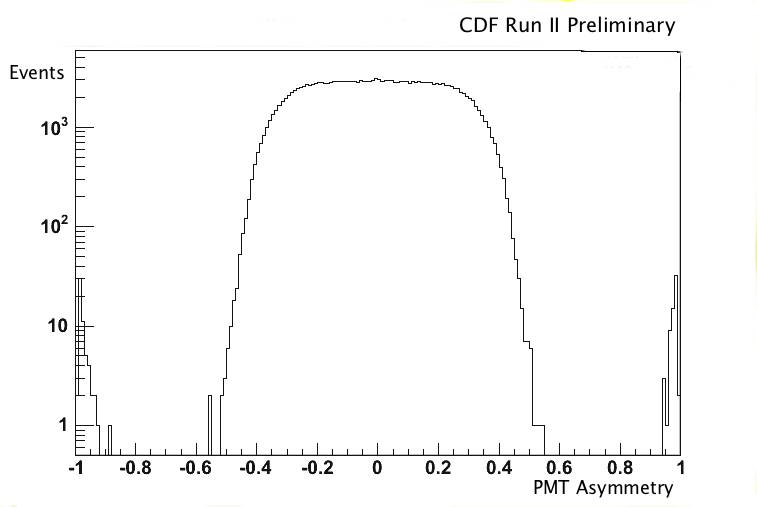
\includegraphics[scale=0.3]{PMT_EM_Asym_twrE_gt_10.jpg}
\caption{PMT Asymmetry observed from EM calorimeter towers with $E>10$~GeV. The clumps at the extremes indicate PMT spikes.}
\label{fig_PMTAsymmetry}
\end{centering}
\end{figure}


\subsection{\halojets}\label{halojets}
This is a another non-collision background that happens to overlap with a real collision. The protons and anti-protons that are not coalesced, upon hitting the beam pipe, create a miniature shower. Only the muons ($\mu$) survive to make it through the beam pipe. These muons (dubbed as \newterm{beam halo}) travel parallel to the beam pipe and interact with the plug and central calorimeters. Such an EM cluster would pass photon-ID cuts (Table \ref{tab:tightphotoncuts}), and making it look like a real photon from the primary collision. It is observed that these muons tends to occupy calorimeter phi wedges 0 and 23 of the CDF detector due the teardrop shape of the colliding beam. The CDF detector experience more halo events in the directions of incoming protons as the D0 detector acts as a filter for the halo originating from antiprotons.

A combination of EM timing cut and a set of topological cuts (see  Table \ref{tab:halocuts}) that are orthogonal to photon-ID cuts (Table \ref{tab:tightphotoncuts}) are used to identify and reject events with a beam halo photon candidate \cite{cdfnote:8409, cdfnote:7960}. Figure \ref{fig:BeamHalo_Identification} shows the beam halo photon candidates isolated by the beam halo ID cuts. Figure \ref{fig:CosmicBeamHaloEMtiming} shows the arrival times of the beam halo and cosmic photon candidates at the EM calorimeter.


\begin{figure}[h]
 \centering
 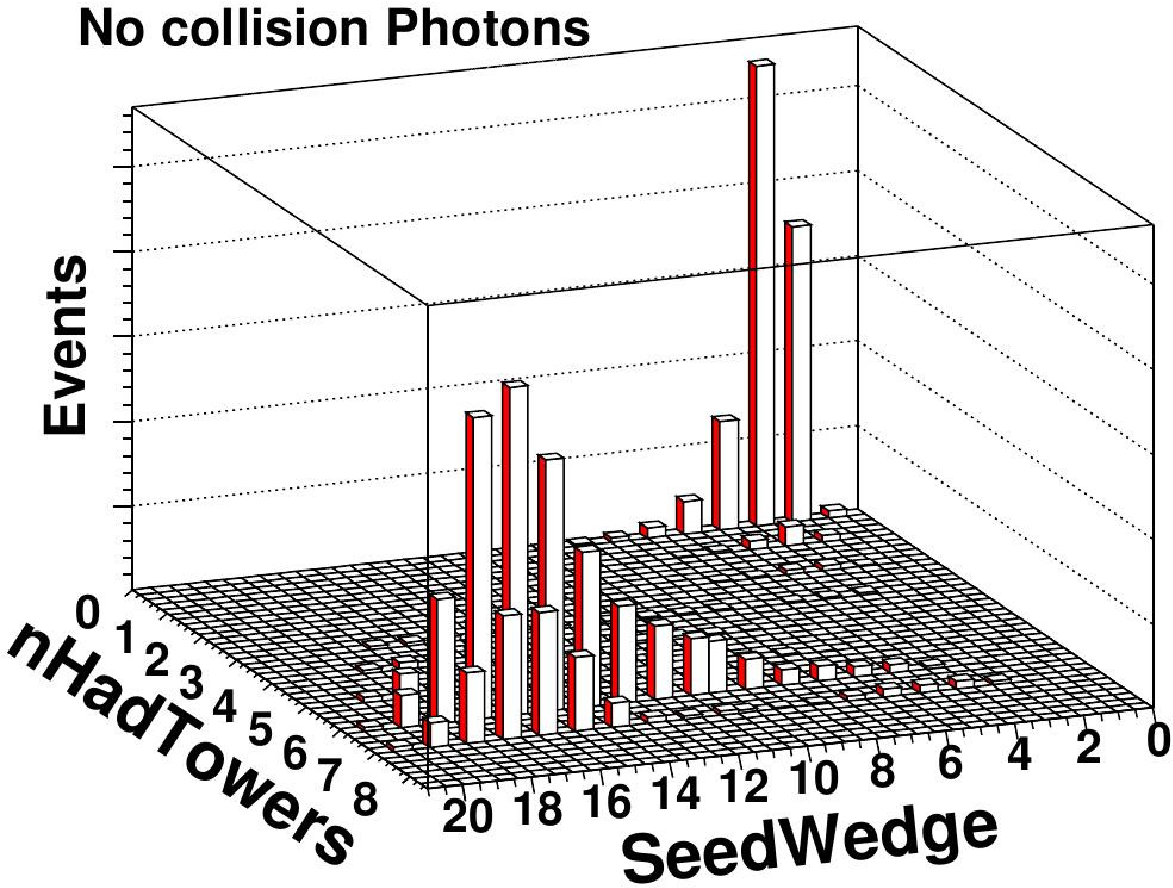
\includegraphics[scale=0.5]{BeamHalo_Topology.pdf}
 % BeamHalo_Topology.pdf: 612x792 pixel, 72dpi, 21.59x27.94 cm, bb=0 0 612 792
 \caption{Beam halo candidates discriminated by the beam halo ID variables. Beam halo candidates tends to have large number of hits in both seed wedge and in the plug hadronic calorimeter.}
 \label{fig:BeamHalo_Identification}
\end{figure}



\begin{figure}[htb!]
 \centering
 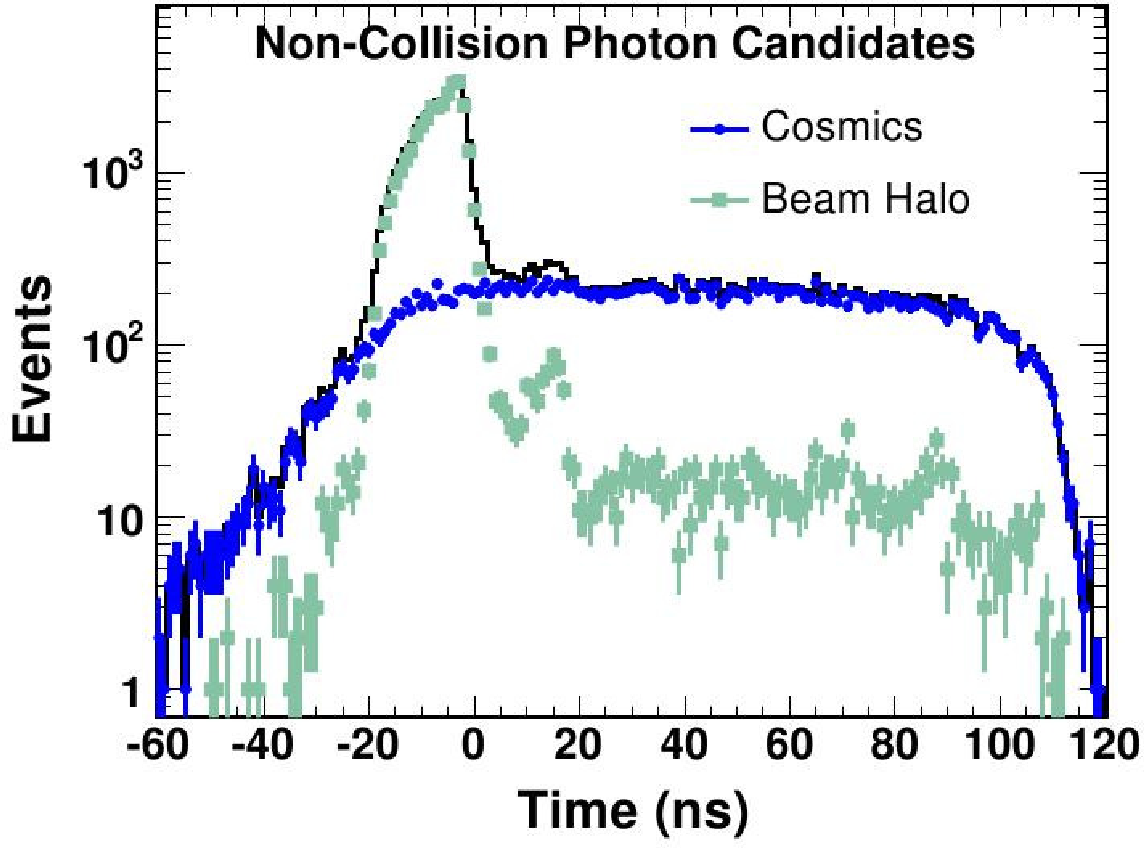
\includegraphics[scale=0.5]{./CosmicBeamHalo_EMtiming.pdf}
 % CosmicBeamHalo_EMtiming.pdf: 612x792 pixel, 72dpi, 21.59x27.94 cm, bb=0 0 612 792
 \caption{EM timing distribution of cosmic and beam halo photon candidates. Photon candidates from the hard scattering process arrive at EM calorimeter around $t=0$~ns. Beam halo photon candidates reaches the EM calorimeter slightly earlier as their path is relatively shorter compared to a photon candidate from a collision. The beam halo photon candidates from the satellite bunches can also be seen in intervals of 18~ns. Cosmic photon candidates are created at a constant rate and is independent of the hard scattering rate. This is indicative by the constant EM timing measurements of cosmic photon candidates.}
 \label{fig:CosmicBeamHaloEMtiming}
\end{figure}

Beam halo ID cuts are used to identify and remove such events from the signal sample. The fraction of such events removed, also known as the  rejection power of the beam halo cuts, is determined by isolating a sample rich in beam halo events and determining fraction of events that can be identified by these cuts.

First select a sample rich in \newterm{beam halo} events that pass modified \newterm{Event Selection} cuts as below.

\begin{enumerate}
 \item Replace the vertex requirement with no vertex (or zero reconstructed vertices). These events with no reconstructed vertex are primarily beam halo and cosmic photon candidate events (see section \ref{sec:cosmicjets}).
 \item Require photon to be within EM timing of \intimewindow.
 \item No requirement on the number of jets.
\end{enumerate}

Apply beam halo ID cuts to this sample of events. Determine the event distribution in phi-wedges of the leading photon candidate before and after applying halo ID cuts. Count events in phi-wedges 0 and 23 and subtract off the flat component (misidentified cosmic photon events and real physics events where a vertex was not reconstructed) estimated from the phi-wedges 1 through 22. Calculate the beam halo rejection power as in equation \ref{eqa:HaloRejectionPower}.

\begin{eqnarray}
 \mathrm{Rejection~Power}~(R^{halo})&=& \frac{N_{0}^{a} - {\bar{N}_{1}^{a} }}{N_{0}^{b} - {\bar{N}_{1}^{b} }}\\
 &=& 94.8\% \nonumber
\label{eqa:HaloRejectionPower}
\end{eqnarray}

\noindent where $N_{0}^{a}$ ($N_{0}^{b}$) is the aggregate events in wedges 0 and 23 after (before) selection cuts and $\bar{N}_{1}^{a}$ ($\bar{N}_{1}^{b}$) is the average number of events in the wedges 1 through 22 after (before) selection cuts.

Hence the percentage of beam halo events that are not rejected or removed is 5.2\%. Multiplying this by the total number of signal events selected using the \newterm{Event Selection} in section \ref{sec:EventSelection} provides an estimate of the probable number of beam halo events not identified and present in the data sample.

As with any set of cuts, beam halo ID cuts will misidentify real photon candidates from primary collision as beam halo photons. This misidentification rate is measured using electrons. This is because electrons are produced often in the collisions and are more readily identifiable by their associated track. First a sample of events with an electron~$\geq 1$~Jets is identified using photon-like electron ID cuts (Table \ref{tab:pecuts}). The electron + jet selection criteria is identical to that of the photon+jets selection. The electron should be \etg{30.0} and \etalessthan{1.1} and the jet should be \etg{15} and \etalessthan{3.0}. Finally apply the beam halo ID cuts to the electron in the events and count the number of events that pass the cuts. Following equation calculates the misidentification rate of the beam halo ID cuts.

\begin{eqnarray}
\mathrm{Beam~halo~Misidentification~Rate}~(M^{halo}) &=& \frac{N_{e+jets}^{a}}{N_{e+jets}^{b}}\\
 &=& 1.2\% \nonumber
\label{eqa:HaloMisIdRate}
\end{eqnarray}

\noindent where $N_{e+jets}^{b}$ total number of identified electron+jets events and $N_{e+jets}^{a}$ is the number of electron+jets events identifies as beam halo candidates (or pass beam halo selection cuts).

The choice of beam halo ID cuts is a compromise between rejection power and misidentification rate. This low misidentification rate is a good choice as almost 95\% of beam halo events are rejected at a loss of only about 1\% of real photon events.

In order to model the distribution (shape) of the remaining beam halo events in the signal sample, a \newterm{template} needs to be made and scaled properly to the expected amount of beam halo events.

A beam halo template is made by selecting data events with the following criteria. This template is normalized (or scaled) to the expected number beam halo events in data (see Table \ref{tab:bgsummary}).

\begin{enumerate}
 \item The run number must be in the good run list.
 \item The event should pass the PHOTON\_25\_ISO, PHOTON\_50 or \mbox{PHOTON\_70} trigger.
 \item No reconstructed vertex.
 \item Require one reconstructed photon with \etg{30} that passes tight photon ID cuts (Table \ref{tab:tightphotoncuts}).
 \item Photon should be in-time (\intimewindow).
 \item Photon should be in phi-wedge 0 or 23.
 \item Pass beam halo ID cuts (Table \ref{tab:halocuts}).
 \item $\geq$1 jets (\etg{15}, \etalessthan{3.0}).
 \item $\Delta \phi(\met - \mathrm{jet})>0.4$
\end{enumerate}


\subsection{\cosmicjets}\label{sec:cosmicjets}
This is a case, a cosmic ray interacts with the calorimeter and bremsstrahlung. These muons are also likely to cross calorimeter towers separated in $\eta$ and $\phi$ from the photon candidate. Hence there is a chance that they will deposit enough energy in those towers to produce a reconstructible soft jet or even another photon.

Cosmic background has a constant rate that is independent of the time of the collision as seen in Figure \ref{fig:CosmicBeamHaloEMtiming}. These events can give rise to really high energy imbalance in the event and hence tends to occupy the large missing energy region. Requiring the arrival time of the photon from the primary collision to be \intimewindow, most of the cosmic photon events are removed. Such events are further identified and removed by identifying muon stubs around cone of the photon candidate  \cite{cdfnote:8409, cdfnote:7960}. First 400~\pbi of Run II data is not used because it does not have EM timing information to reject this background efficiently. The remaining cosmic photon events are estimated using the EM timing distribution of the photon in tight \phojets as in equation \ref{eqn:cosmicEstimate}. Data events are selected similar to the \newterm{Event Selection} in section \ref{sec:EventSelection} with the exception of EM timing of the photon to be within \cosmictimewindow.

\begin{equation}
\mathrm{Cosmic~photon~estimate}~(D^{cosmic}) = \frac{N_{30-90}^{cosmic}}{90~\mathrm{ns} - 30~\mathrm{ns}} \times (4.8~\mathrm{ns}\times2)
\label{eqn:cosmicEstimate}
\end{equation}

where $N_{30-90}^{cosmic}$ is the number of photon+jets events with EM timing of the photon between 30--90~ns.

This simple equation counts the number of cosmic photon candidate events in the time window between \cosmictimewindow and then extrapolate it to the \intimewindow time window where the data events are selected from. Table \ref{tab:bgsummary} lists the expected number of cosmic events.

A template for this background is made with the following selection rules and it is normalized to the expected number of events in Table \ref{tab:bgsummary}.

\begin{enumerate}
	\item The run number must be in the good run list.
	\item The event should pass the \firstphotrig, \secondphotrig, and \thirdphotrig.
	\item There should be at least one good class 12 vertex.
	\item The $z$-coordinate of the highest-\pt vertex should be within the well-instrumented region, i.e. \mbox{$|z|<60$~cm}.
	\item Require one reconstructed photon with \etg{30} that passes tight photon ID cuts (see Table \ref{tab:tightphotoncuts}).
	\item Photon should be between \cosmictimewindow.
	\item $\geq$1 jets (\etg{15}, \etalessthan{3.0}).
	\item $\Delta \phi(\met - \mathrm{jet})>0.4$
\end{enumerate}

\section{Standard Model Backgrounds}\label{sec:SMbackgrounds}

\subsection{\elejets}\label{sec:elejets}
This is a standard model background where a lepton is misidentified as a photon. This can happen in two ways.

\begin{enumerate}
\item {A lepton as it traverse the detector radiates a photon and recoils and this photon is identified as the prompt photon.}
\item {Failure to reconstruct the associated track of a lepton.}
\end{enumerate}

The later case is less significant than the first. This fake probability varies with the energy of the lepton. Most of these leptons come from $\w^{\pm}$ decay to leptons. Less significant contributions come from $Z$, and di-boson decays to leptons. Partial tracks of such leptons are traced and matched using outside-in track reconstruction. This algorithm tries to find calorimeter energy deposition with hits in the silicon detector and COT, and also known as ``Phoenix'' track reconstruction for historical reasons.  The Phoenix track finding algorithm is about 60\% effective in rejecting leptons with energies \etg{30}. An electron candidate passing tight electron ID cuts in the central EM calorimeter with \etg{30} faking a tight photon candidate after rejecting electron with phoenix track is $<0.007$ and decreases rapidly as the energy of the electron \cite{CDF8220}.

The distribution of the remaining \elejets events are modeled using  electroweak Monte Carlo data. First select events that has a tight photon candidate and jets in electroweak Monte Carlo data according to the criteria listed below.

\begin{enumerate}
	\item The run number must be in the good run list.
	\item There should be at least one good class 12 vertex.
	\item The $z$-coordinate of the highest-\pt vertex should be within the well-instrumented region, i.e. \mbox{$|z|<60$~cm}.
	\item Require one reconstructed photon with \etg{30} that passes tight photon ID cuts (see Table \ref{tab:tightphotoncuts}).
	\item Reject if a track is found (or a ``phoenix photon'')
	\item $\geq$1 jets (\etg{15}, \etalessthan{3.0}).
	\item $\Delta \phi(\met - \mathrm{jet})>0.4$
\end{enumerate}

Events passing above criteria is selected from each of the \zee, \zmm, \ztt, \wen, \wmn, and \wtn Monte Carlo datasets. These samples or events selected from these are collectively called electroweak (EWK).

Additional corrections for these events are derived to correctly model the underlying event and multiple interaction as described in section \ref{sec:ewkMCcorrections}. The total EWK background with the corrections is defined as in equation \ref{eqa:EWKtotalWeighted}.

\begin{equation}
\mathrm{EWK} = \mathrm{EWK}_{Z}^{MC}\times f_{vertex}^{Z+jets} + \mathrm{EWK}_{W}^{MC}\times f_{vertex}^{W+jets}\times f_{\met}^{W+jets}
\label{eqa:EWKtotalWeighted}
\end{equation}

Finally, events from each electroweak sample is scaled to total integrated luminosity of the data using the equation \ref{eqn:MCDATAscaleByLum}. Each sample's cross section is corrected for next-to-leading order contributions by an additional standard constant multiplier called `k-factor', $k=1.4$. Individual samples are added according to equation \ref{eqa:EWKtotalWeightedLumScaled} to make the total EWK prediction.

\begin{center}
\begin{equation}
\mathrm{Scale}~(S^{lum}) = \mathrm{\frac{Total~Integrated~Luminosity~of~Data}{Luminosity~of~Monte~Carlo~Data}} = \frac{{\cal L}^{Data}}{{\cal L}^{MC}}
\label{eqn:MCDATAscaleByLum}
\end{equation}
\end{center}

\begin{equation}
\mathrm{EWK} = f_{vertex}^{Z+jets} \displaystyle\sum_{i} {MC_{Z_{i}}\times S^{lum}_{i}} +
f_{vertex}^{W+jets}\times f_{\met}^{W+jets} \displaystyle\sum_{j} {MC_{W_{j}}\times S^{lum}_{j}}
\label{eqa:EWKtotalWeightedLumScaled}
\end{equation}

where $i$ is the summation over \zee, \zmm, and \ztt and $j$ is the summation over \wen, \wmn and \wtn MC samples respectively.

\subsection{Di-photon production}\label{sec:diphoton}
This is a SM process where a pair of photons is produced in the primary collision. The production mechanism (or the Feynman diagrams) are different from SM \phojets. But the processes are not 100\% distinguishable at detector level. One of the photons produced will be identified as the prompt photon and the second photon or a soft jet from underlying event, will be identified as a jet during the event selection. Although the cross section is smaller by orders of magnitude, the significance of this background is the higher probability to completely loose one of the photons into a crack in the detector (an uninstrumented region). About 15\% if the CDF detector is uninstrumented hence the probability of loosing one of these photons increases up to 30\%. If a photon is lost in a crack that event would most likely to appear as a high \met event. This is exactly where new particles search is most sensitive.

The distribution of this irreducible background is modeled using diphoton Monte Carlo data. Events satisfying the \newterm{Event Selection} (section \ref{sec:EventSelection}) is chosen and scaled to data by luminosity using the equation \ref{eqn:MCDATAscaleByLum}. Prior to scaling, these events are corrected for underlying events and multiple interaction by reweighing by the vertex distribution of photon+jets data and diphoton Monte Carlo data. Final prediction for diphoton background is described in equation \ref{eqa:diPhoFinal}

\begin{eqnarray}
\mathrm{Total~diphoton~prediction} &=& f_{vertex}^{diphoton}\times MC_{diphoton} \times S^{lum}
 \nonumber\\
&=& f_{vertex}^{diphoton}\times MC_{diphoton} \times \frac{{\cal L}^{Data}}{{\cal L}^{diphoton~MC}}
\label{eqa:diPhoFinal}
\end{eqnarray}

\subsection{QCD Background}\label{sec:QCDbackground}
These are events where jets from light mesons decay into photons. \pizero, $\rho$ and $\eta$ particles are produced often and their branching ratio to two photons are almost 100\%. If the two photons are less energetic the CES detector can be used to discriminate them and hence remove event from selection. If the two photons produced are energetic, CES is not able resolve them and they would be reconstructed as a single photon. In such case the hits (ADC counts or the MIPs) in the CPR detector is used to identify and rejected such events. The photon ID cuts requirement on isolation energy, second CES cluster, and $\chi^{2}$ (Table \ref{tab:tightphotoncuts}) suppresses this background significantly. This jet fake rate is about $\sim$10E-4 at 30~GeV and decreases rapidly with increasing jet energy.

A sample of events that fails to pass tight photon ID cuts but pass loose photon ID cuts (photon-sideband or sideband-photons) are chosen  to model the fake jets in the signal sample. Most of the fake jets in signal sample are from quarks whereas the sideband photons are mostly gluons. This is because of the extra color carried by the gluons creating extra particles in a larger region of the detector and hence would often fail isolation requirement and fail to pass tight photon ID cuts.

The following selection criteria is used to derive the shape of this background.
\begin{enumerate}
	\item The run number must be in the good run list.
	\item The event should pass the PHOTON\_25\_ISO, PHOTON\_50 or \mbox{PHOTON\_70} trigger.
	\item There should be at least one good class 12 vertex.
	\item The $z$-coordinate of the highest-\pt vertex should be within the well-instrumented region, i.e. \mbox{$|z|<60$~cm}.
	\item Require one reconstructed photon with \etg{30} that passes loose photon ID cuts and fails tight photon ID cuts (Tables \ref{tab:loosephotoncuts} and \ref{tab:tightphotoncuts}).
	\item Photon should be in-time, \intimewindow.
	\item Reject if identified as a phoenix photon.
	\item Reject if identified as a beam halo candidate .
	\item $\geq$1 jets (\etg{15}, \etalessthan{3.0}).
	\item $\Delta \phi(\met - \mathrm{jet})>0.4$
\end{enumerate}

\noindent From the CES/CPR weight, the fake photon fraction for photons with \etg{30} is determined to be 0.319 $\pm$ 0.001(stat) $\pm$ 0.068(syst). After subtracting cosmic, beam halo, electroweak, and diphoton backgrounds from data, the remainder is split between QCD and SM prompt photons according to this fraction. The electroweak, beam halo, and cosmic backgrounds in the sideband events are subtracted prior to scaling to remove the double counting of such events. This QCD template is scaled as in equation \ref{eqa:QCDscale}.

\begin{equation}
\mathrm{QCD~Normalization}(C^{QCD}) = \frac{N^{data}-N^{halo+cosmic+ewk+diphoton}}{N^{qcd}}\times 0.319
\label{eqa:QCDscale}
\end{equation}

\noindent where $N^{data}$ is the total number of data events selected using the \newterm{Event Selection} in section \ref{sec:EventSelection},   $N^{halo+cosmic+ewk+diphoton}$ is the sum of all other background events except QCD and SM photon+jets, and $N^{qcd}$  is the total number of sideband events selected using afore mentioned \newterm{Event Selection}.


\subsection{SM Prompt Photon + Jets}\label{sec:SMpromptPhotonJets}
The SM prompt \phojets production is modeled using Monte Carlo data and by using the \newterm{Event Selection} described in section \ref{sec:EventSelection}. With inclusion of this signal, it is assumed the data is understood and described by the SM. This sample of events is normalized using photon fraction as mentioned under section \ref{sec:QCDbackground}. From CES/CPR method, ``fake photon fraction + true photon fraction = 100\% of photon data'', implies that the ``true photon fraction = 1.0 - fake photon fraction''. Hence this template is scaled as in equation \ref{eqa:QCDscale}.

\begin{equation}
\mathrm{Normalization} (C^{SM~photon}) = \frac{N^{data}-N^{halo+cosmic+ewk+diphoton}}{N^{SM~photon}}\times(1.0- 0.319)
\label{eqa:SMpromptScale}
\end{equation}

\noindent where $N^{data}$ is the total number of data events selected using the \newterm{Event Selection} in section \ref{sec:EventSelection},   $N^{halo+cosmic+ewk+diphoton}$ is the sum of all other background events except QCD and SM photon+jets, and $N^{SM~photon}$ is the total number of sideband events selected using the same \newterm{Event Selection} as described in section \ref{sec:EventSelection}.

Total prediction of this background is defined as below.
\begin{eqnarray}
\mathrm{Total~SM~photon~prediction} &=& f_{vertex}^{photon}\times MC_{photon} \times C^{SM~photon}
\label{eqa:PhoFinal}
\end{eqnarray}

\noindent where $f_{vertex}^{photon}$ is the additional correction for multiple interactions and underlying event as describe in section \ref{sec:MCcorrectionsUEMI}, and $MC_{photon}$ is the total number of events selected from photon MC data using the \newterm{Event Selection} in section \ref{sec:EventSelection}.

This normalization scheme forces the total number of signal (data) events selected to be equal to the sum of all background events. And hence any discrepancy observed between data and total background prediction will result in a shape difference indicating physics beyond SM. This is summarized in the equation below.

\begin{equation}
 N^{data} = N^{SM photon}+N^{qcd}+N^{diphoton}+ N^{EWK}+N^{cosmic}+N^{beam~halo}
\end{equation}
\noindent where $N$ is the total number of events in a given sample (after proper normalization). The distributions made using this formula will be referred to as \newterm{Default Method} or \newterm{Method A}.


\section{Correcting MC Samples for Underlying Event and Multiple Interactions}\label{sec:MCcorrectionsUEMI}
The Monte Carlo data samples used in this analysis does not cover the complete data periods. Which means they do not have the correct modeling of instantaneous luminosity. This can significantly affect the measurements, especially \met measurement.

\subsection{Electroweak MC Samples}\label{sec:ewkMCcorrections}
A set of weights is derived as a function of number of vertices ($N_{vtx}$) by comparing $W$+jets events and $Z$+jets events in data to Monte Carlo data.

In generating weights for $W$ and $Z$ Monte Carlo events, first, electrons are identified using photon-like electron ID cuts (Table \ref{tab:pecuts}).

Events with $W$+jets are selected as follow.

\begin{enumerate}
 \item Require a good reconstructed vertex.
 \item Select a photon-like electron with \etg{20.0} and \etalessthan{1.1}
 \item \metg{20.0}
 \item Reconstruct a $W$ candidate from above electron and \met
 \item Require the reconstructed $W$ candidate to have \ptg{30.0}, \etalessthan{1.1}, and transverse mass $60~\mathrm{GeV/c}^{2}<M_{T}^{W}<100~\mathrm{GeV/c}^{2}$.
 \item $\geq$1 jet with \etg{15.0} and \etalessthan{3.0}
 \item $\Delta \phi(\met - \mathrm{jet})>0.4$
\end{enumerate}

The idea of this selection is to use $W$ to represent the leading photon and hence exact identical cuts on \pt and $\eta$. The transverse mass cut is required to suppress the background processes for \wjets events. The vertex and \met distributions in \wjets data and \MC is compared. Vertex distributions are normalized to unity and then data to \MC ratio is taken. The \met distribution is normalized by luminosity prior to taking data to \MC ratio. These weights are used to reweight all the $W$ \MC samples. Total weight is:

\begin{equation}
 \mathrm{Weight,}~f^{W+jets} = f_{vertex}^{W+jets} \times f_{\met}^{W+jets} = \frac{N^{W+jets~data}_{vtx}}{N^{W+jets~MC}_{vtx}} \times \frac{\met^{W+jets~data}}{\met^{W+jets~MC}}
 \label{eqa:WjetsWeights}
\end{equation}

\noindent where $N_{vtx}^{W+jets}$ is the fraction of events per given vertex bin and $\met^{W+jets}$ is the number of events for a given \met bin.

Similarly, \zjets events are selected as below and weights are generated by data and \MC comparison. But \met weights are not included as the statistics were too low.

\begin{enumerate}
 \item Require a good reconstructed vertex.
 \item Select two photon-like electrons with \etg{20.0} and require one to be in \etalessthan{1.1}. Second electron may be in \etalessthan{3.0}
 \item Reconstruct a $Z$ candidate from above electrons
 \item Require the reconstructed $Z$ candidate to have \ptg{30.0}, \etalessthan{1.1}, and mass to be $76~\mathrm{GeV/c}^{2}<M_{Z}<106~\mathrm{GeV/c}^{2}$.
 \item $\geq$1 jet with \etg{15.0} and \etalessthan{3.0}
 \item $\Delta \phi(\met - \mathrm{jet})>0.4$
\end{enumerate}

The total weight for any $Z$ MC sample is:

\begin{equation}
 \mathrm{Weight,}~f^{Z+jets}_{vertex}= \frac{N^{Z+jets~data}_{vtx}}{N^{Z+jets~MC}_{vtx}}
 \label{eqa:ZjetsWeights}
\end{equation}

\noindent where $N_{vtx}^{Z+jets}$ is the fraction of events per given vertex bin.

%[Z+JETS NVTX AND MET WEIGHTS GOES HERE]

\subsection{Photon MC and Di-photon MC}\label{sec:phoMCcorrections}
The photon and di-photon Monte Carlo samples' vertex distributions ($N_{vtx}$) are compared to photon data and \MC events are weighted to match the vertex distribution of data.

Photon+jets events are selected from data, photon MC and diphoton MC as described under the \newterm{Event Selection} in section \ref{sec:EventSelection}. The vertex distribution in each sample is normalized to unity and data-to-photon MC and data-to-diphoton MC ratios are taken. Finally the photon and diphoton MC events are weighted by their corresponding vertex weight.

The total weight for photon MC events is:
\begin{equation}
 \mathrm{Weight,}~f_{vertex}^{photon} = \frac{N_{vtx}^{\gamma+jets~Data}}{N_{vtx}^{\gamma+jets~photon~MC}}
 \label{eqa:diphojetsWeights}
\end{equation}

The total weight for diphoton MC events is:
\begin{equation}
 \mathrm{Weight,}~f_{vertex}^{diphoton} = \frac{N_{vtx}^{\gamma+jets~Data}}{N_{vtx}^{\gamma+jets~diphoton~MC}}
 \label{eqa:phojetsWeights}
\end{equation}

\noindent where $N_{vtx}$ is the fraction of events per given vertex bin.

%%%%%%%%%%%%%%%%%%%%%%%%%%%%%%%%%%%%%%
\section{Alternate Background Prediction}\label{sec:AltBgPrediction}

It became evident the leading-order \MC data was inadequate to model some of the kinematic distributions. Specifically transverse energies of the leading jets and other kinematic variables that directly depends on it (eg. \Ht, \met) were not well described. An alternate background modeling was developed to overcome this using a reweighted sideband photon candidate sample. This indirectly replaces SM photon \MC data sample with the sideband photon data sample.

The technique involves reweighting photon \et spectrum of the photon sideband sample to match the sum of photon sideband and photon \MC data events using the equation \ref{eqa:sidebandReweighting}. The weights are derived as a function of \et of the sideband-photon candidates.


\begin{center}
 \begin{eqnarray}
  \nonumber
  w &=& \frac{\epsilon.MC+(1-\epsilon) SB}{SB}\\
  \Delta w &=& (\frac{MC}{SB}-1)\Delta \epsilon
 \label{eqa:sidebandReweighting}
 \end{eqnarray}
\end{center}


\noindent where
%\begin{center}
\begin{eqnarray}
  \nonumber
  w &=& \mathrm{Weight~for~sideband\textendash photon~to~be~reweighted}\\ \nonumber
  MC &=& \mathrm{Photon~\MC~data events~for~a~given~histogram~bin}\\ \nonumber
  SB &=& \mathrm{Sideband\textendash photon~data~events~for~a~given~histogram~bin}\\ \nonumber
 \epsilon &=& \mathrm{True~photon~fraction~as~described~in~section~\ref{sec:SMpromptPhotonJets}}\\ \nonumber
 \Delta w &=& \mathrm{Propagated~uncertainty~of}~w\\ \nonumber
  \Delta\epsilon &=& \mathrm{Uncertainty~of~the~true~photon~fraction}\\ \nonumber
\end{eqnarray}
%\end{center}

The reweighing can also be explained by the following equation.
\begin{equation}
 \mathrm{Total~Background\simeq \epsilon\times~photon~\MC+(1-\epsilon)\times~photo\textendash sideband}
\end{equation}


The sideband-photon sample has all the higher order contributions that are missing the photon \MC data as it is from real data. This was clearly observed in the jet multiplicity distribution. There the photon-sideband described the data perfectly. Though the photon-sideband is used to represent the fake photons (jets) in the data from tight photon selection, it is derived from a different set of Feynman diagrams. In fact, most of the sideband-photons are gluon jets. The fake photons in tight selection is mostly quark jets. Furthermore, the default background prediction method described the photon \et spectrum well. Hence by reweighing photon-sideband to match the total background prediction in photon \et spectrum should allow to use next-to-leading order physics in sideband-photon sample without a significant change to the underlying physics.

The following equation shows the normalization of the background samples when this reweighted photon sideband sample is used to describe the data.

\begin{equation}
 N^{data} = N^{qcd~weighted}+N^{diphoton}+N^{EWK}+N^{cosmic}+N^{beam~halo}
\end{equation}

where $N$ is the total number of events in a given sample (after proper normalization). The distributions made using this formula will be referred to as \newterm{Method B}.


\section{Systematics Uncertainties}

We have accounted for the following systematic uncertainties. We combine the individual systematic uncertainties in quadrature to construct the error band in the final plots.

\subsection{\cosmicjets}
We choose a smaller time window within the cosmic time window (\cosmictimewindow) and make another prediction of the number of cosmic events left in the sample. The difference between the predictions is taken as the systematic uncertainty.

\subsection{\elejets}
We take the uncertainty in the integrated luminosity of the electroweak Monte Carlo event sample to measure the systematic uncertainty of the electroweak backgrounds, which is $\sim$6\% (This is excluding the uncertainty in the PDFs). We vary the normalization by this uncertainty which gives a different shape for the curve. The difference in the shapes is taken as the systematic uncertainty for the electroweak background.

\subsection{\halojets}
The systematic uncertainty for beam halo is taken to be 50\%  of the bin content, as this background is insignificant at this stage of the analysis.


\subsection{Fake and Real Photon Fraction}
We use 100\% of the photon sideband sample to predict the shape of the jet multiplicity. This technique is suitable as the jet multiplicity is independent of the photon \et and hence the photon sideband describes this distribution very well. Other histograms are generated using a combination of the photon sideband and the pure photons to get the correct shape. The relative normalization of the sideband and pure photons is determined a priori using the CES/CPR method~\cite{wwwCESCPR}. The fake photon fraction for photons with \etg{30} is calculated to be 0.319 $\pm$ 0.001(stat) $\pm$ 0.068(syst). We apply this fraction to the whole sample, not on an event-by-event basis.

There is no correlation between the QCD background fraction and the true photon fraction from the photon Monte Carlo. The fake photon fraction is used to get the shape and the normalization correct.

Where we have used the 100\% of the sideband sample, we apply the following prescription to estimate the systematic uncertainty.

\begin{enumerate}
\item Notice that there are four selection ID variables common to both loose photon ID cuts (Table~\ref{tab:loosephotoncuts})  and tight photon ID cuts (Table~\ref{tab:tightphotoncuts}):  Had/EM, Isolation Energy, Track \pt and Track Isolation.
\item Tighten up the loose ID cuts to match the tight photon ID cuts, one at a time.
\item Run the sideband sample through the new set of cuts.
\item Normalize the number of events that pass to the number of events in the standard sideband sample.
\item Divide the variable (histogram) by the corresponding standard sideband variable (histogram).
\item Plot all four histograms obtained by varying the four cuts  on the same histogram for each kinematic variable.
\item Take the maximum variation in each bin to be the systematic uncertainty for that bin.
\end{enumerate}

In the case where we use the mixture of the sideband and the photon Monte Carlo, we vary the mixture within the fake photon fraction's systematic uncertainty to obtain an alternate normalization, and hence a different shape of the curve. We then take the shift in shape to be the systematic  uncertainty due to the fake photon photon fraction.

\subsection{Jet Energy Scale}
We account for jet energy mismeasurement by varying the the jet energy up and down by $\pm \sigma$. We remake the histograms with the shifted jets and take the maximum deviation from the central value as the systematic uncertainty due to jet energy scale and resolution. This is the largest contributor to the final systematic uncertainty.

\subsection{EM Energy Scale}
This is to account for the EM energy mismeasurement of the EM objects. We shift the the photon energy by 1\% along with the jet energy scale and take the deviation from the central value as the systematic uncertainty.

\subsection{PDF Uncertainty}
Uncertainty in modeling the parton distribution functions in Monte Carlo data sample is estimated following the standard CDF prescription described in CDF note 7051~\cite{CDF7051}. This method is a less strenuous way of obtaining PDF uncertainty. (Other option is to generate 40 MC samples by varying 20 eigen vectors) In this method we reweight CTEQ5L (Leading order) MC events to CTEQ6M (Next-to-leading order) and derive 40 variations (or weights) of 20 eigen vectors. Each pair of (up and down) variation is compared to the reference (or base) to derive a ratio. Maximum variations of each eigen vector is added in quadratures to derive the final PDF systematic for PDF uncertainty.

\subsection{$\alpha _{s}$ Uncertainty}
Uncertainty on strong coupling constant in MC sample is derived by comparing CTEQ5L nominal to the MRST98LO base sample. CTEQ5L MC events were weighted using the MRST98LO base and the ratio is included in total systematics.

\subsection{ISR/FSR Uncertainty}
This uncertainty is due to thresholds set for the initial and final state radiation (or the amount of radiation in the parton shower). In reality there is no upper limit or lower limit on the amount of radiation emitted from incoming or out going partons. Following the recommendations of Joint Physics group \footnote{http://www-cdf.fnal.gov/internal/physics/joint\_physics/agenda/20050527-minutes.html} we generated 4 additional \textsc{Pythia} MC samples by changing \textsc{Pythia} parameters (Sudakov Form Factors) and compare to a base sample. These samples are generator level only. We identify prompt photon using PDG code and use hadron level jets to reproduce the  final kinematic distribution and derive variations. Maximum variation is of each pair of samples is taken and added in quadratures to the total systematics.
%--explain the stitching process

\subsection{Q-scale Uncertainty}
Additional \textsc{Pythia} MC samples are generated by doubling the Q value in \textsc{Pythia} and reducing by half. Samples were generated with different pt-hat s. These samples are generator level only. We identify photon using leading photon using PDG code and use hadron level jets to reproduce the  final kinematic distributions and derive variations.

\subsection{Statistical Uncertainty in the Background Estimation}
Statistical uncertainty becomes significant in the high end tail of some variables due to limited statistics in the background expectations. Hence we have incorporated the statistical uncertainty into the final systematic error.

\subsection{Uncertainty in deriving the Alternate weighted-QCD sample}
When this weighted sideband is used to make the total background prediction, in addition to all of the systematic errors mentioned so far, uncertainty in the reweighting process is included. It is calculated by deriving an alternate weight ($w+\Delta w$) using error propagation as shown in equation \ref{eqa:sidebandReweighting}. The difference between background predictions from nominal weight ($w$) and alternate weight ($w+\Delta w$) is taken as the systematic uncertainty.

% \subsection{Additional Systematic error from \newterm{Method A} and \newterm{Method B}}
% We derive additional uncertainty for the total background by taking the difference between the \newterm{Method A} and \newterm{Method B} background predictions. And this error is applied to both methods and becomes the dominant uncertainty in almost all the distributions.\newline


\section{Summary of Background Estimates}
Following tables summarize the total background predictions for different data samples. Sum of individual backgrounds for a given event sample will add up to total number of data events for that sample.

%%%%%%%%%%%%%%%%%%%% Background Summary for g+jets sample %%%%%%%%%%%%%
\begin{table}[h!]
\begin{center}
\begin{tabular} {|c|c|c|}
\hline
\bf{Background} & \bf{Expected for $\gamma+\geq$1 Jet} & \bf{Expected for $\gamma+\geq$2 Jets} \\
\hline
SM Photon  	& 6,774,250 & 1,313,330 \\
\hline
QCD		& 2,944,903 & 493,176 \\
\hline
EWK		& 23,530 & 3,666 \\
\hline
Di-photon 	& 24,272 & 3,550 \\
\hline
Cosmic 		& 131 & 7 \\
\hline
Beam Halo	& 1 & $<$1\\
\hline
PMT Spikes  	&  0 & 0 \\
\hline
\end{tabular}
\end{center}
\caption{Summary of background estimates for \phojets event sample.}
\label{tab:bgsummary}
\end{table}


%%%%%%%%%%%%%%%%%%%% Background Summary for g+jets+met>20 sample %%%%%%%%%%%%%
\begin{table}[h!]
\begin{center}
\begin{tabular} {|c|c|c|}
\hline
\multirow{2}{*} {\bf Background} & \bf{Expected for} & \bf{Expected for}\\
& {\bf $\gamma+\geq$1 Jet+\metCorr$>$20~GeV} & {\bf $\gamma+\geq$2 Jets+\metCorr$>$20~GeV}\\

\hline
SM Photon  	& 201,396 & 66,241\\
\hline
QCD		& 53,535 & 15,538\\
\hline
EWK		& 12,542 & 1,686\\
\hline
Di-photon 	& 710 & 173\\
\hline
Cosmic 		& 124 & 8\\
\hline
Beam Halo	& 0 & 0\\
\hline
PMT Spikes  	&  0 & 0 \\
\hline
\end{tabular}
\end{center}
\caption{Summary of background estimates for \phojets+\metCorr$>$20~GeV event sample.}
\label{tab:bgsummary}
\end{table}

\section{Search for Resonance Decay}
The invariant masses of final state decay products are searched for a resonance (bump) assuming a null hypothesis. Under null hypothesis the assumption is there is no resonance production (or bump). Which means there should be no significant deviation of data in any region of the mass distribution compared to any other region.

For this a $\chi^{2}$ statistical test if performed and it is defined as below.

\begin{equation}
 \chi^{2} = \sum \frac{({\cal O}_{k} - E_{k})^{2}}{\sqrt{E_{k}}}
 \label{eqa:chi2Stat}
\end{equation}

where for a given bin $k$, ${\cal O}_{k}$ is the number of observed data events and $E_{k}$ is the expected number of events. The idea is that the number of data events per bin (${\cal O}_{k}$), should have an average value of $E_{k}$ and would be expected to fluctuate around $E_{k}$ with a standard deviation of order$\sqrt{E_{k}}$. If $\chi^{2}=0$, the agreement between observed and the expected distribution is perfect meaning for all bins $k$, ${\cal O}_{k}=E_{k}$. In general if the $\chi^{2}\leq n$ where $n$ is the number of bins, the observed and expected distributions agree reasonably well and no bump can be claimed. If the $\chi^{2}>>n$, the  observed and the expected distributions differ significantly and possible bump exists.

\section{Results}
The kinematic distributions for the $\gamma+\geq 1$ jet, $\gamma+\geq 2$ jet, $\gamma+\geq 1$ jet+\metCorr$>20$~GeV, and $\gamma+\geq 2+$\metCorr$>20$~GeV are shown in Figures \ref{fig:Result_MtdA_gj1_PhoEt} through \ref{fig:Result_MtdB_gj2_Mass_gj1j2}.
Figures \ref{fig:Result_MtdA_gj1_PhoEt} through \ref{fig:Result_MtdA_gj2_Mass_gj1j2} are made according to \newterm{Method A}. Figures \ref{fig:Result_MtdB_gj1_PhoEt} through \ref{fig:Result_MtdB_gj2_Mass_gj1j2} are made according to \newterm{Method B}. The difference in two methods can be noticed by the absence of color \newterm{pink} in the \newterm{Method B} histograms.

Both \newterm{Method A} and \newterm{Method B} have their strengths and weaknesses. \newterm{Method A} describes almost all the distributions very well except \newterm{$H_{T}$}, \newterm{NJet} and \newterm{\met}. And \newterm{Method B} shows weakness in describing invariant mass distributions. \newterm{Method B} is derived to aid and better understand some of the next-to-leading order effects that is not well modeled by Monte Carlo data.
%The two methods can be used further understand the differences in color flow as they represent two different Feynman diagrams.

Figured xxx-xxx shows the fits to the various mass distributions in \phoonejet and subsamples. The search for a narrow resonance in various mass distributions do not show significant fluctuations.

\section{Additional Studies Requiring SecVtx Tag Jets}
We performed additional studies using the data from same photon data stream (\textbf{c}) and using data up to and including period 30 (${\cal L} = 5.7~\mathrm{fb}^{-1})$. We use the same kinematic selections and in addition require jets to have SevVtx tag (or $b$-tag). The 3 additional subsamples are:

\begin{enumerate}
  \item $\gamma$ + $\geq 1 b$-Jet.
  \item $\gamma$ + $\geq 2 b$-Jets. This required two $b-$tag jets. Subsequent jets are not checked for a tag.
  \item $\gamma$ + $\geq 2$~Jets where only one of the two jets required to have a tag. Subsequent jets are not checked for a tag.
\end{enumerate}

\section{Conclusions}
All the measured distributions have shown good agreement with the Standard Model expectation. There was no significant deviation observed between data and the background expectation. Further more the search for resonance decay has shown no significant fluctuations.

\section{Acknowledgments}
We like to thank Shin-Shan Eiko Yu providing us with the fake photon fraction and for all the advice. Also, we want to thank Max Goncharov for answering various questions and providing the run-dependent EM timing corrections.


\begin{thebibliography}{99}

\bibitem{CDF8220} CDF--8220, R. Culbertson {\it et al.}, ``Probability of an Electron Faking an Isolated Prompt Photon in CEM'', May 30, 2006.

\bibitem{CDF9224} CDF--9224, S. Hewamanage {\it et al.}, ``Validation of Photon Sample by Estimating \wen and  \zee  Cross Sections'', March, 2008.

\bibitem{wwwJER} CDF Jet Energy and Resolution Group, ``http://www-cdf.fnal.gov/internal/physics/top/ jets/corrections.html''.

\bibitem{wwwCESCPR} CES/CPR method for Photon background from Photon group, ``http://www-cdf.fnal.gov/internal/physics/photon/docs/CesCprMethod.html''

\bibitem{CDF7051} CDF--7051, Oscar Gonzalez, Carsten Rott, ``Uncertainties due to the PDFs for the gluino-sbottom search'', June, 2004.

\bibitem{cdfnote:7960}``Methods for Determining the Photon Event Rates and Timing Distributions for Searches with Final State Photons'', M. Goncharov, V. Krutelyov, D. Toback, and P. Wagner, R. Culbertson, A. Pronko, CDF note 7960

\bibitem{cdfnote:8409}``Discrimination of Beam Halo and Cosmic Rays as a Source of Photon Candidates'', M. Goncharov, V. Krutelyov, D. Toback, and P. Wagner, R. Culbertson, A. Pronko, CDF note 8409

\bibitem{cdfnote:9184}``Search for Anomalous Production of \pho\pho+\met Events in 2~\fbi of Data'', R. Culbertson, A. Pronko, M. Goncharov et.al., CDF note 9184


\end{thebibliography}

\clearpage
%\newpage

\begin{figure}[h!]
 \centering
\subfigure[]{
 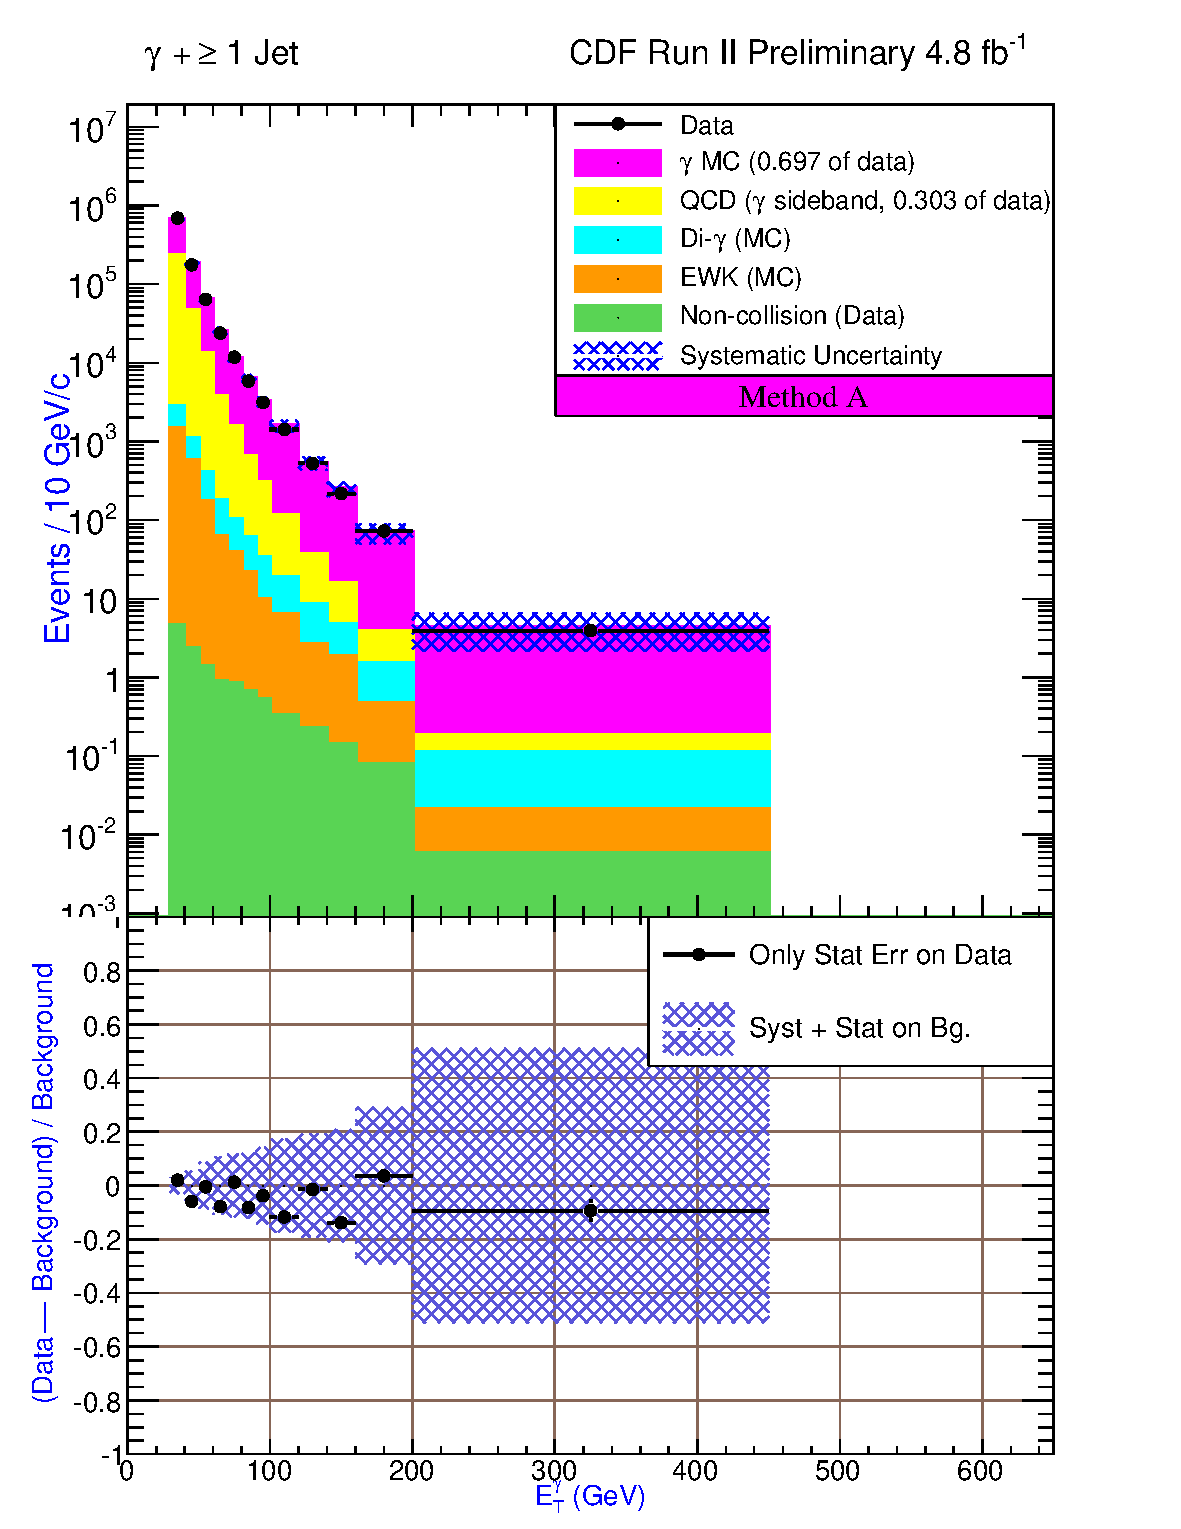
\includegraphics[scale=\resultsHistScale,keepaspectratio=true]{./g30jet_MtdA_plot1_Et_pho.pdf}
 % g30jet_MtdA_plot1_Et_pho.pdf: 567x734 pixel, 72dpi, 20.00x25.89 cm, bb=0 0 567 734
}
\subfigure[]{
 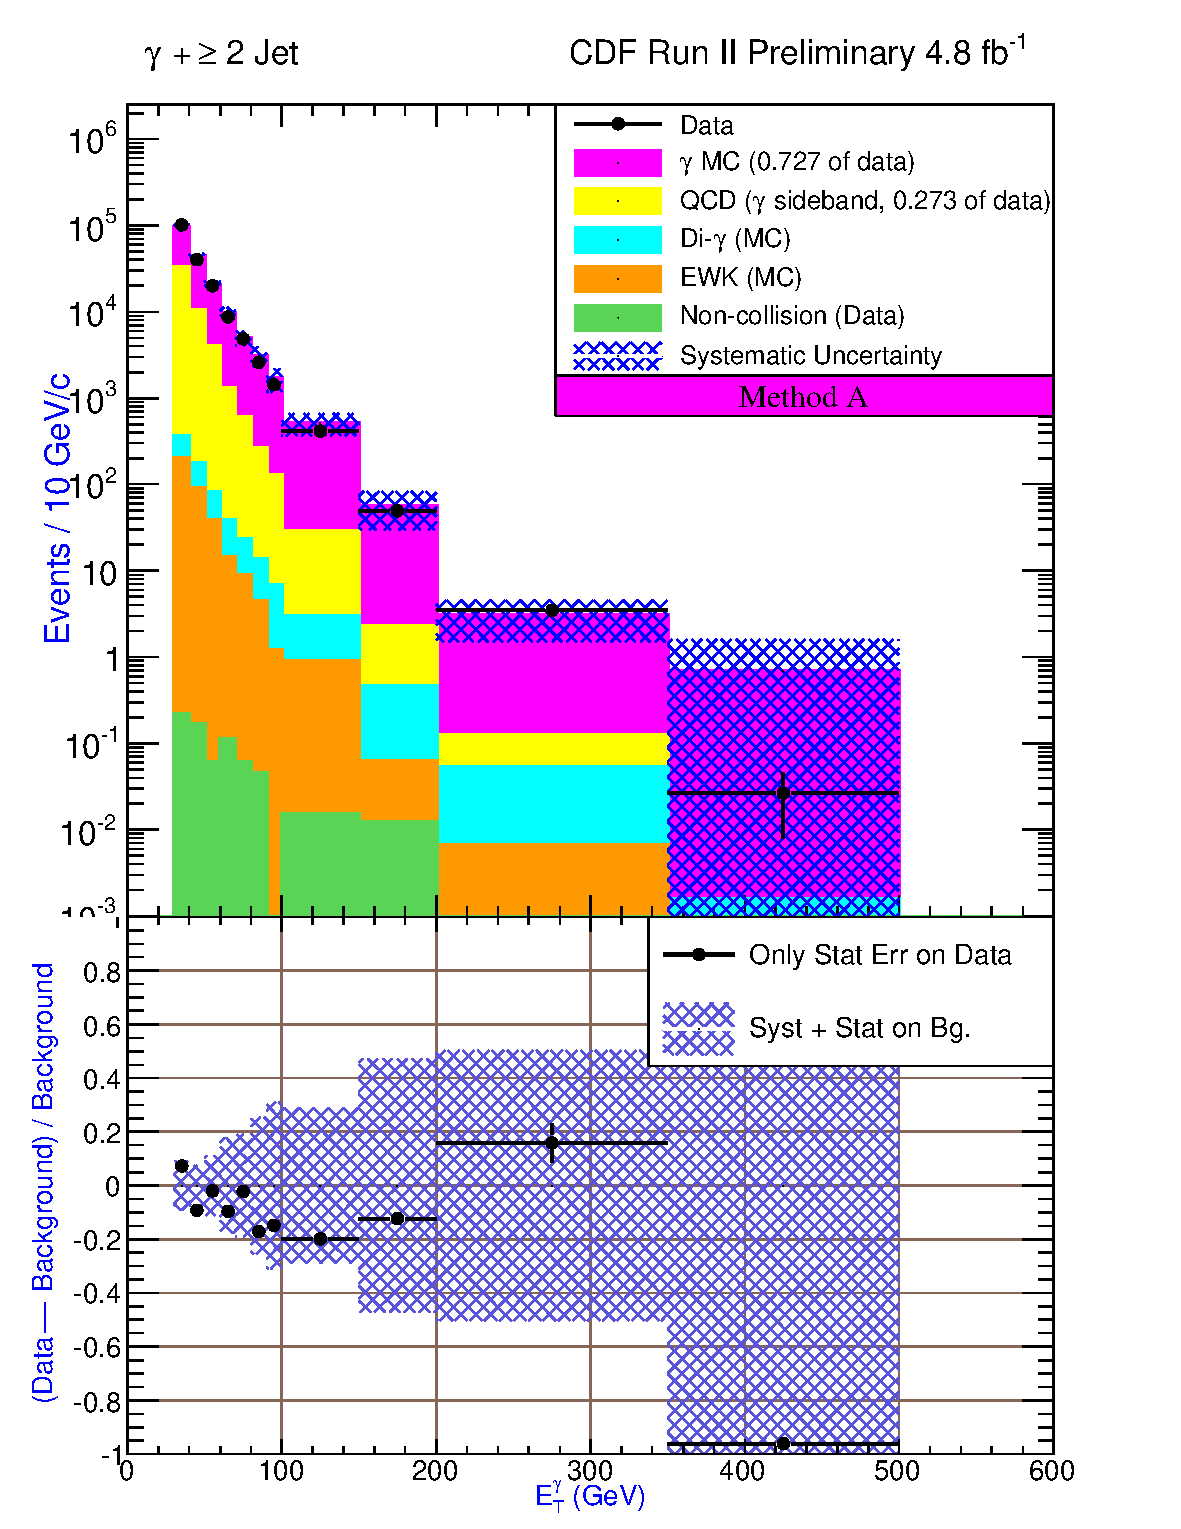
\includegraphics[scale=\resultsHistScale,keepaspectratio=true]{./g30jet_MtdA_plot2_Et_pho.pdf}
 % g30jet_MtdA_plot1_Et_pho.pdf: 567x734 pixel, 72dpi, 20.00x25.89 cm, bb=0 0 567 734
}

 \caption{\newterm{Method A}: Photon \et distribution of the \phoonejet (left) and \photwojet (right) data samples.}
 \label{fig:Result_MtdA_gj1_PhoEt}
\end{figure}

\begin{figure}[h!]
 \centering
\subfigure[]{
 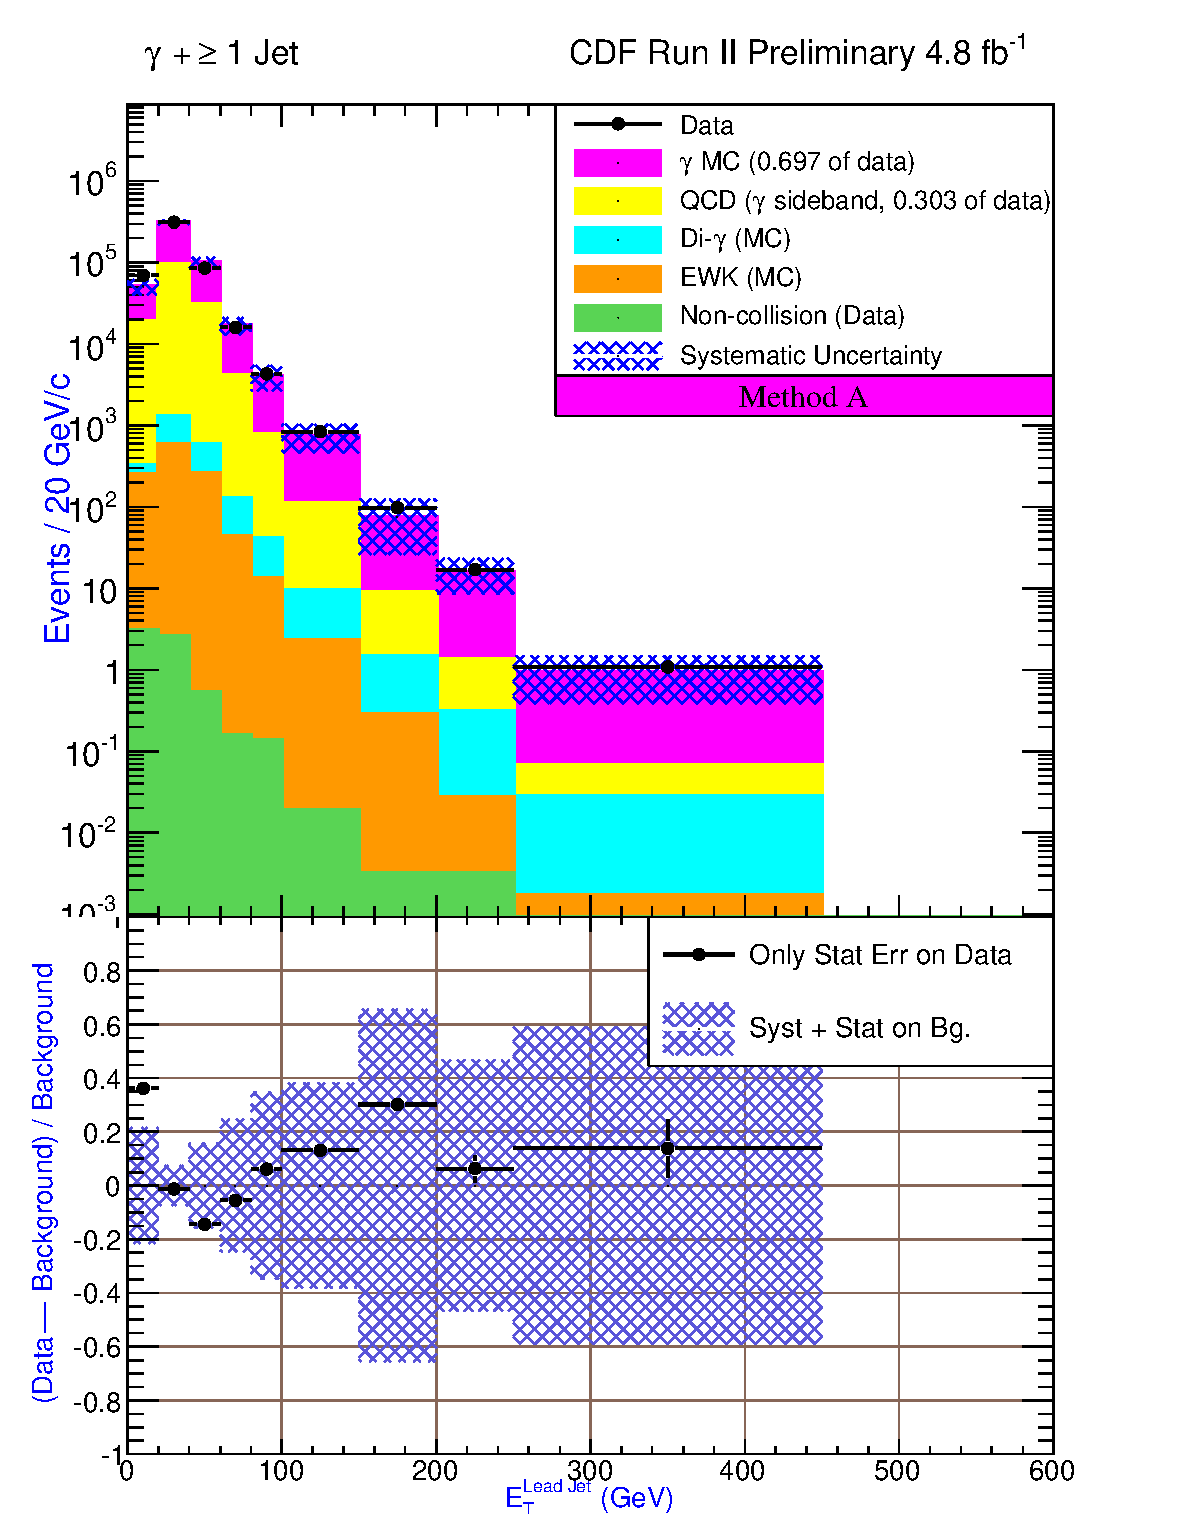
\includegraphics[scale=\resultsHistScale,keepaspectratio=true]{./g30jet_MtdA_plot1_Et_j1.pdf}
 % g30jet_MtdA_plot1_Et_pho.pdf: 567x734 pixel, 72dpi, 20.00x25.89 cm, bb=0 0 567 734
}
\subfigure[]{
 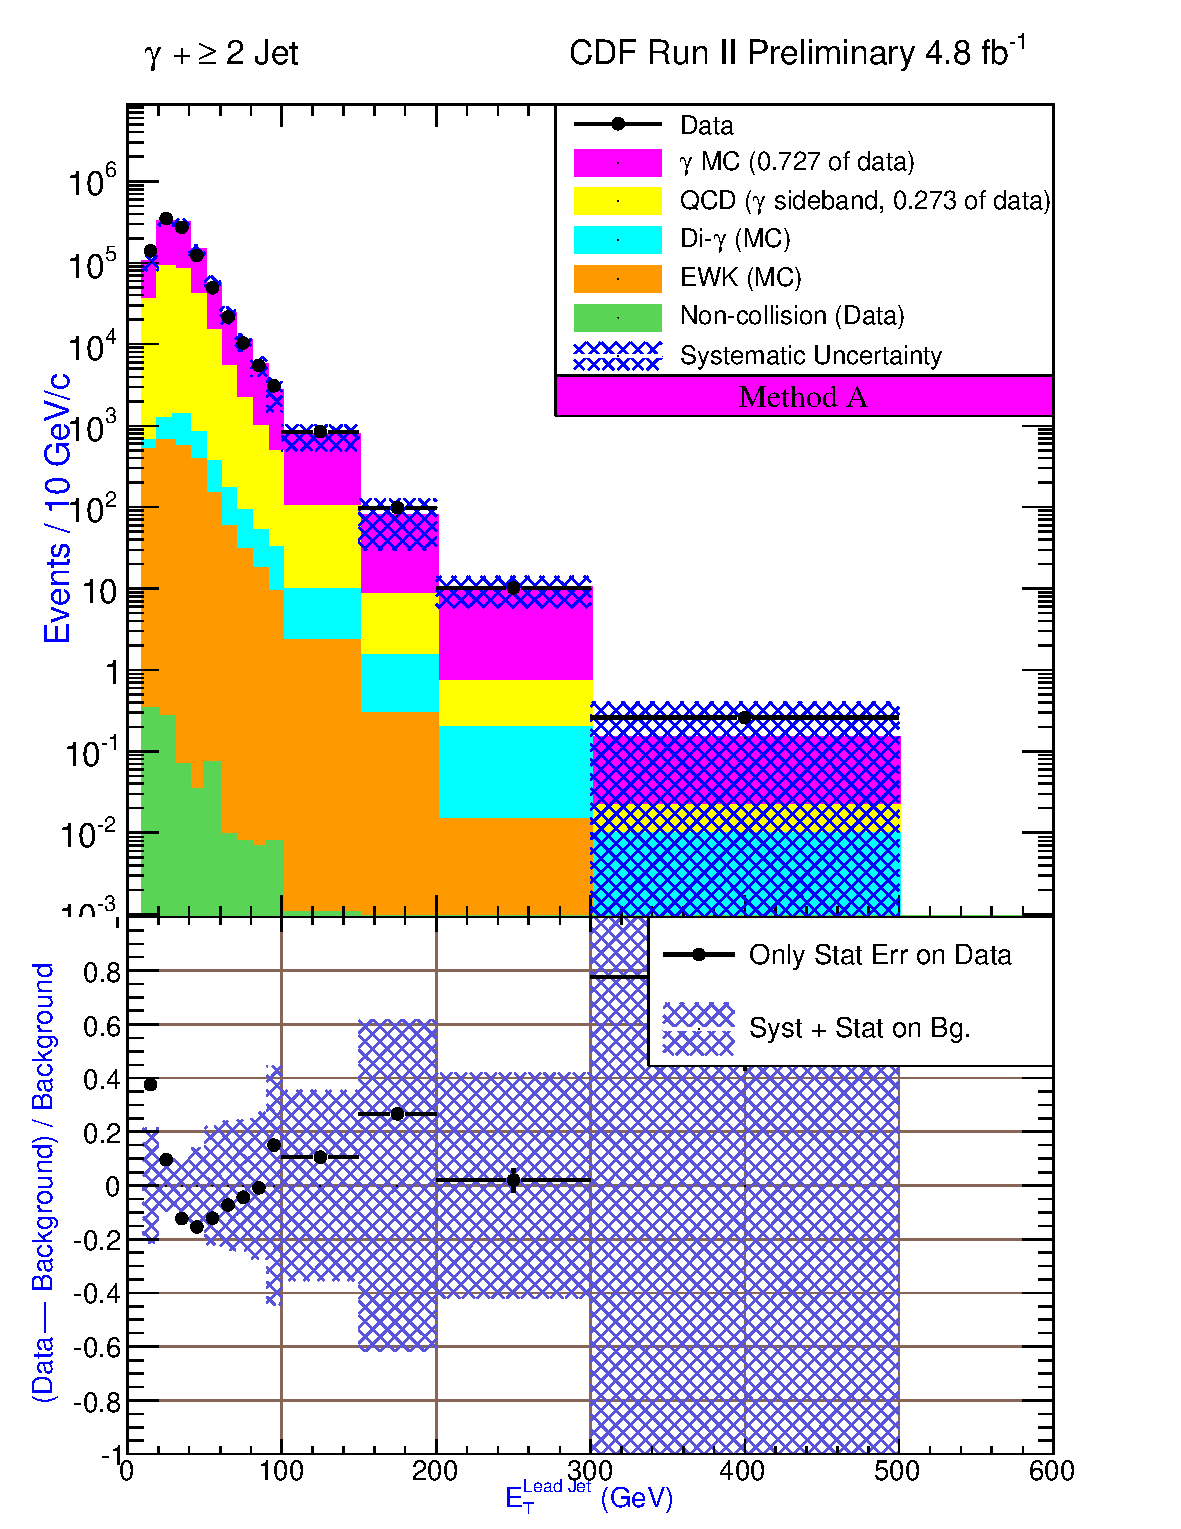
\includegraphics[scale=\resultsHistScale,keepaspectratio=true]{./g30jet_MtdA_plot2_Et_j1.pdf}
 % g30jet_MtdA_plot1_Et_pho.pdf: 567x734 pixel, 72dpi, 20.00x25.89 cm, bb=0 0 567 734
}
 \caption{\newterm{Method A}: \et distribution of the leading jet in \phoonejet (left) and \photwojet (right) data samples.}
 \label{fig:Result_MtdA_gj1_JetEt}
\end{figure}

\begin{figure}[h!]
 \centering
 \subfigure[]{
 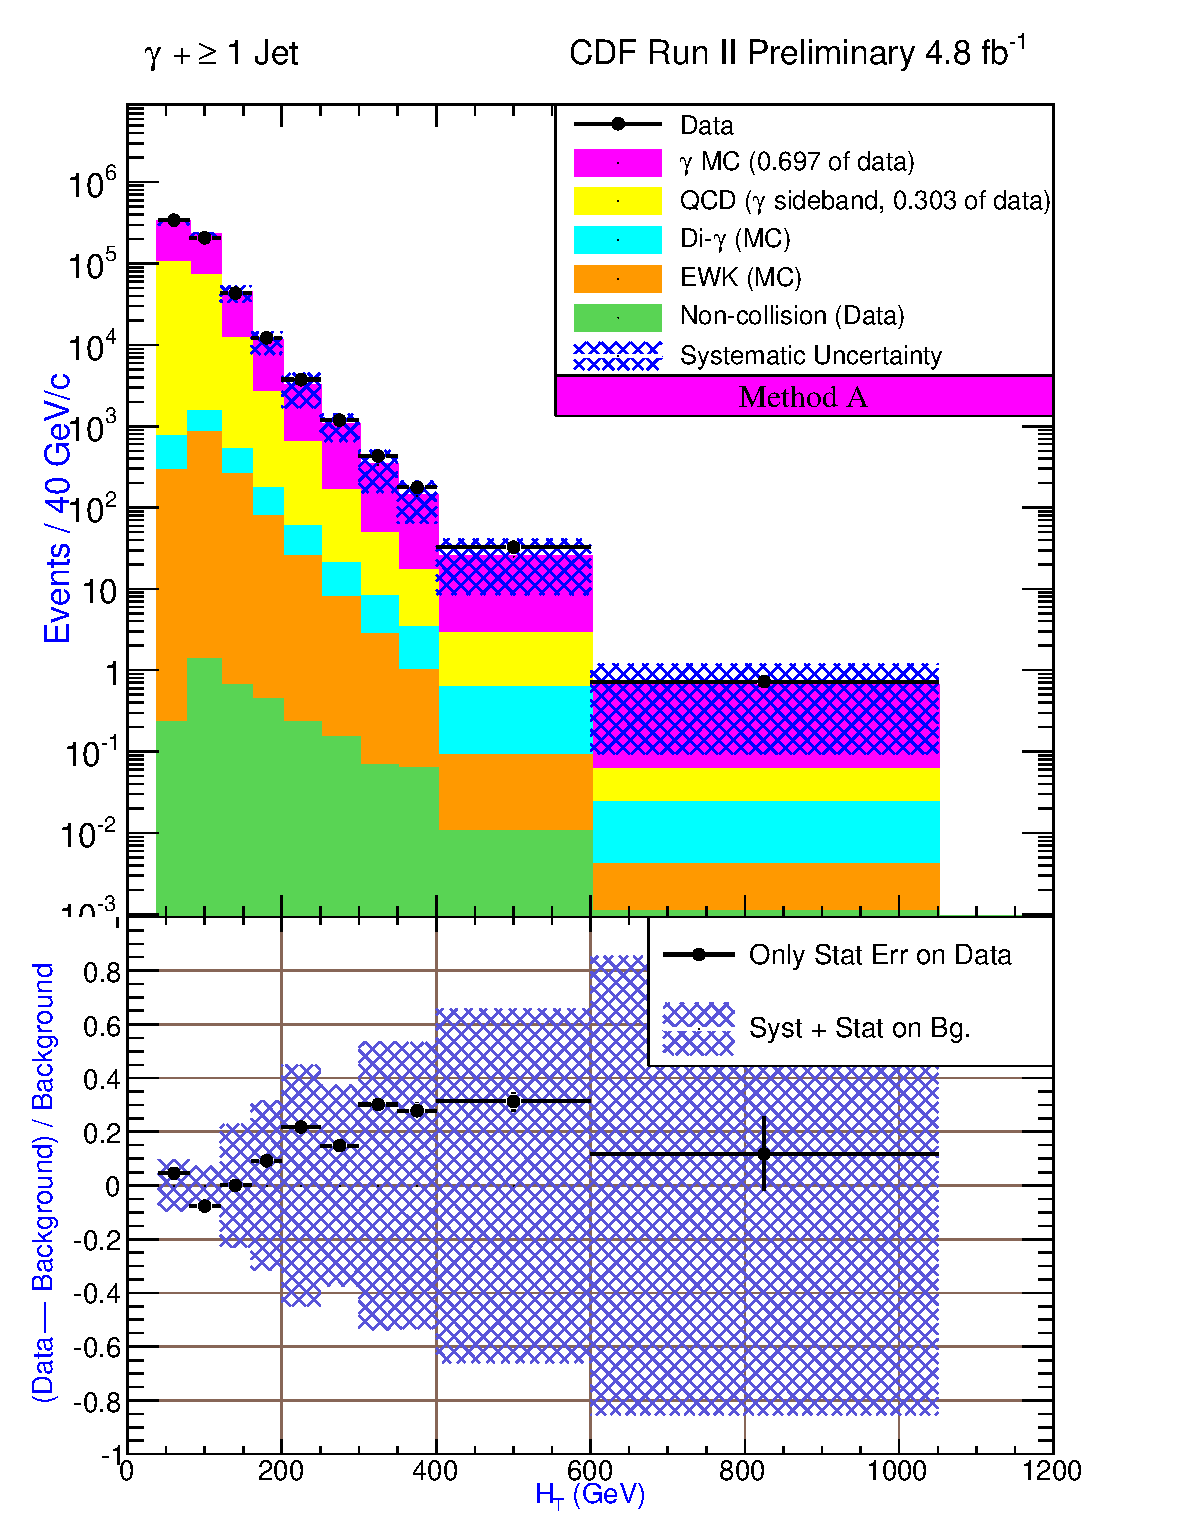
\includegraphics[scale=\resultsHistScale,keepaspectratio=true]{./g30jet_MtdA_plot1_Ht.pdf}
 % g30jet_MtdA_plot1_Et_pho.pdf: 567x734 pixel, 72dpi, 20.00x25.89 cm, bb=0 0 567 734
}
 \subfigure[]{
 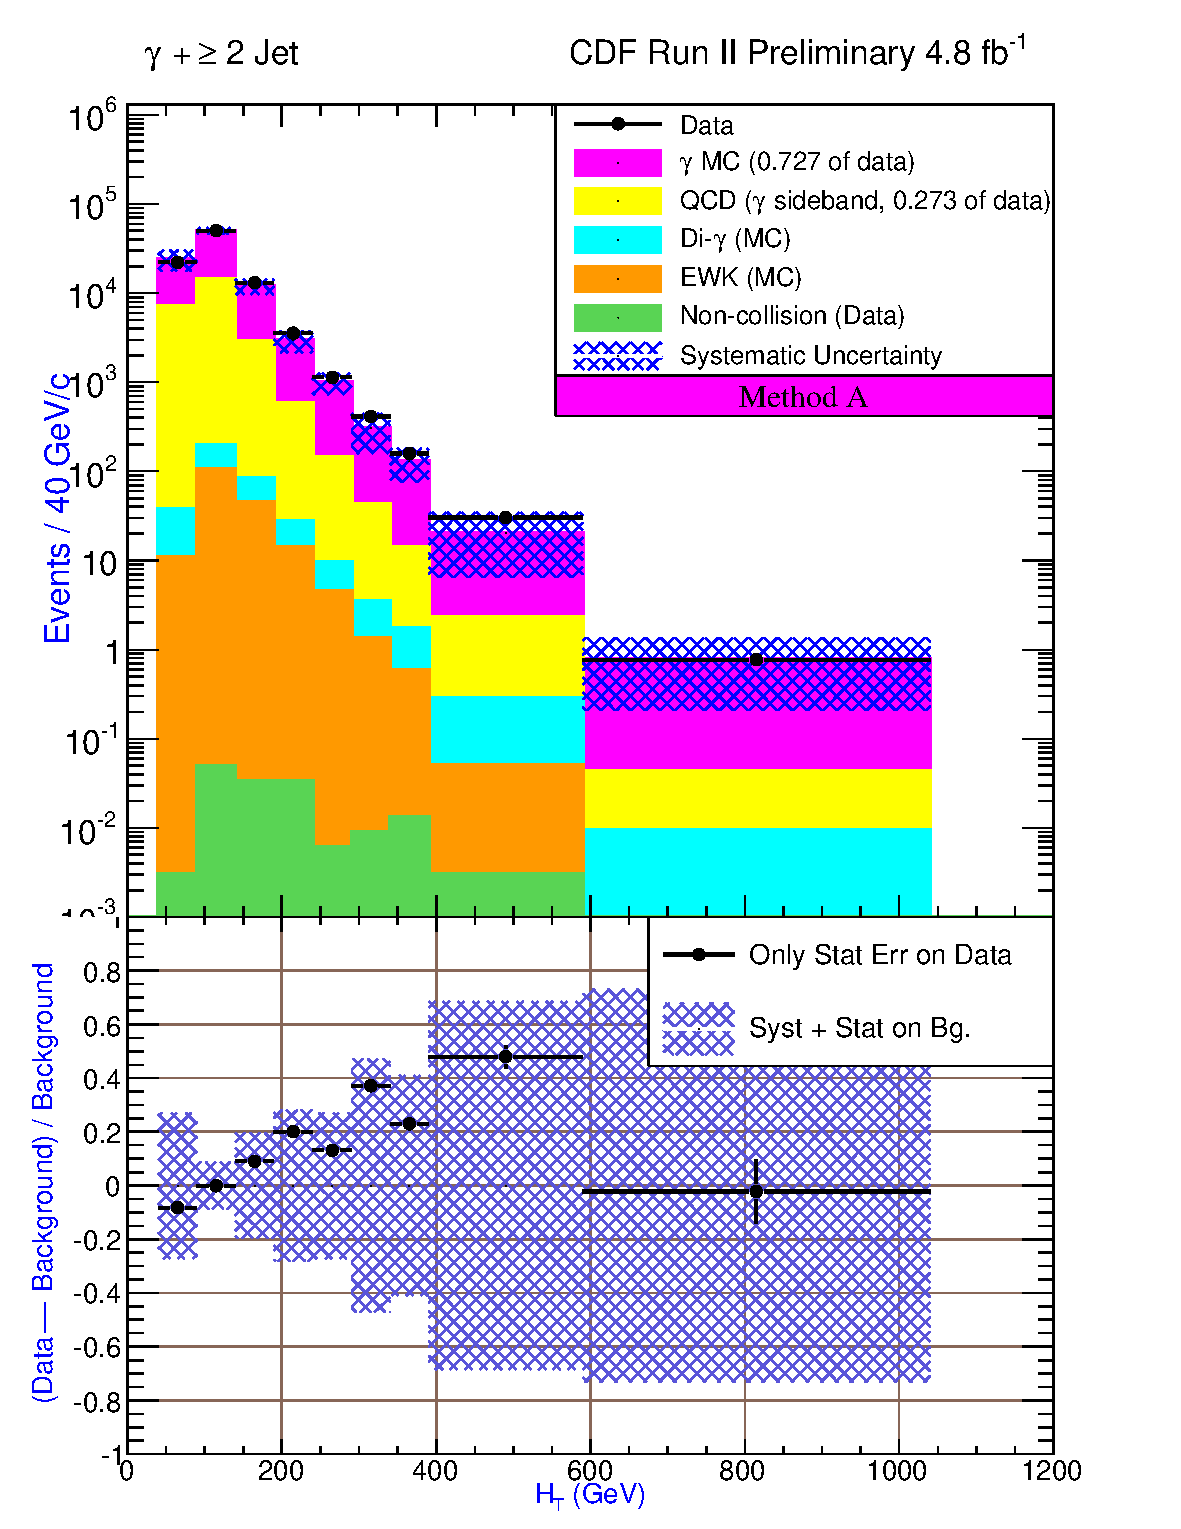
\includegraphics[scale=\resultsHistScale,keepaspectratio=true]{./g30jet_MtdA_plot2_Ht.pdf}
 % g30jet_MtdA_plot1_Et_pho.pdf: 567x734 pixel, 72dpi, 20.00x25.89 cm, bb=0 0 567 734
}
 \caption{\newterm{Method A}: \Ht distribution of the leading jet in \phoonejet (left) and \photwojet (right) data samples.}
 \label{fig:Result_MtdA_gj1_Ht}
\end{figure}

\begin{figure}[h!]
 \centering
\subfigure[]{
 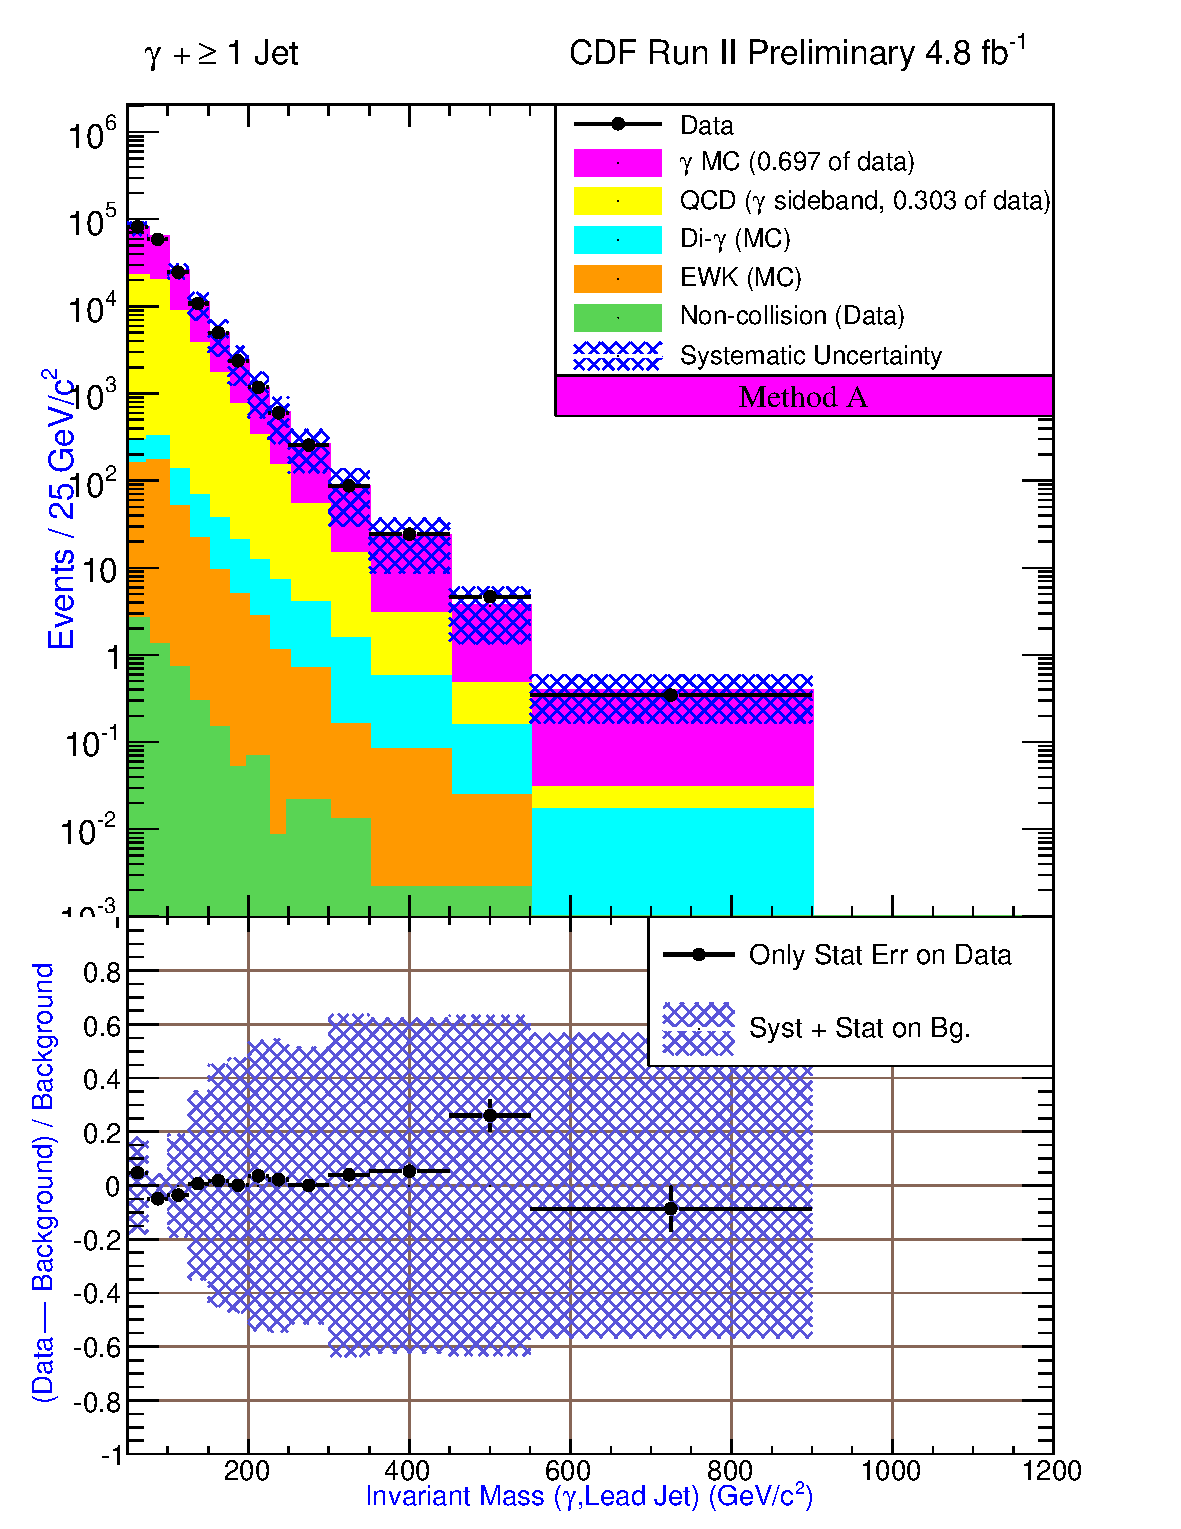
\includegraphics[scale=\resultsHistScale,keepaspectratio=true]{./g30jet_MtdA_plot1_InvMass_pj1.pdf}
 % g30jet_MtdA_plot1_Et_pho.pdf: 567x734 pixel, 72dpi, 20.00x25.89 cm, bb=0 0 567 734
}
\subfigure[]{
 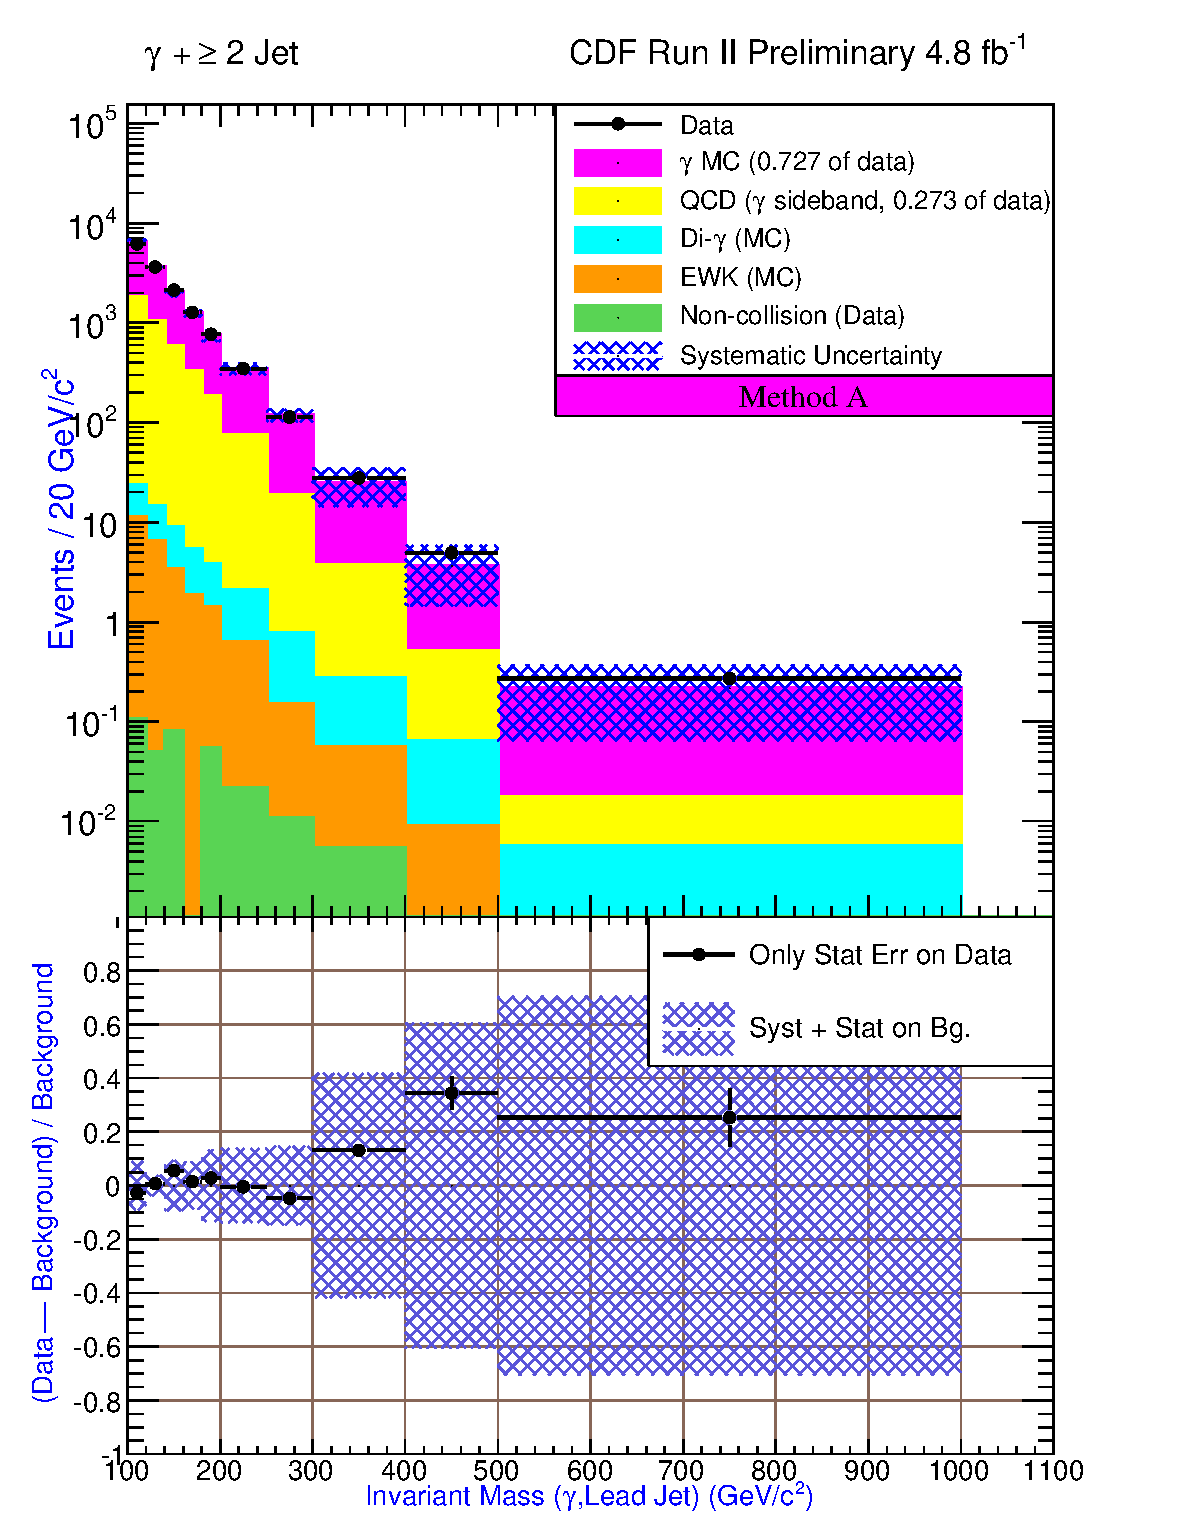
\includegraphics[scale=\resultsHistScale,keepaspectratio=true]{./g30jet_MtdA_plot2_InvMass_pj1.pdf}
 % g30jet_MtdA_plot1_Et_pho.pdf: 567x734 pixel, 72dpi, 20.00x25.89 cm, bb=0 0 567 734
}
 \caption{\newterm{Method A}: Invariant mass of the photon and the leading jet distributions of the leading jet in \phoonejet (left) and \photwojet (right) data samples.}
 \label{fig:Result_MtdA_gj1_Mass_gj1}
\end{figure}

\begin{figure}[h!]
 \centering
\subfigure[]{
 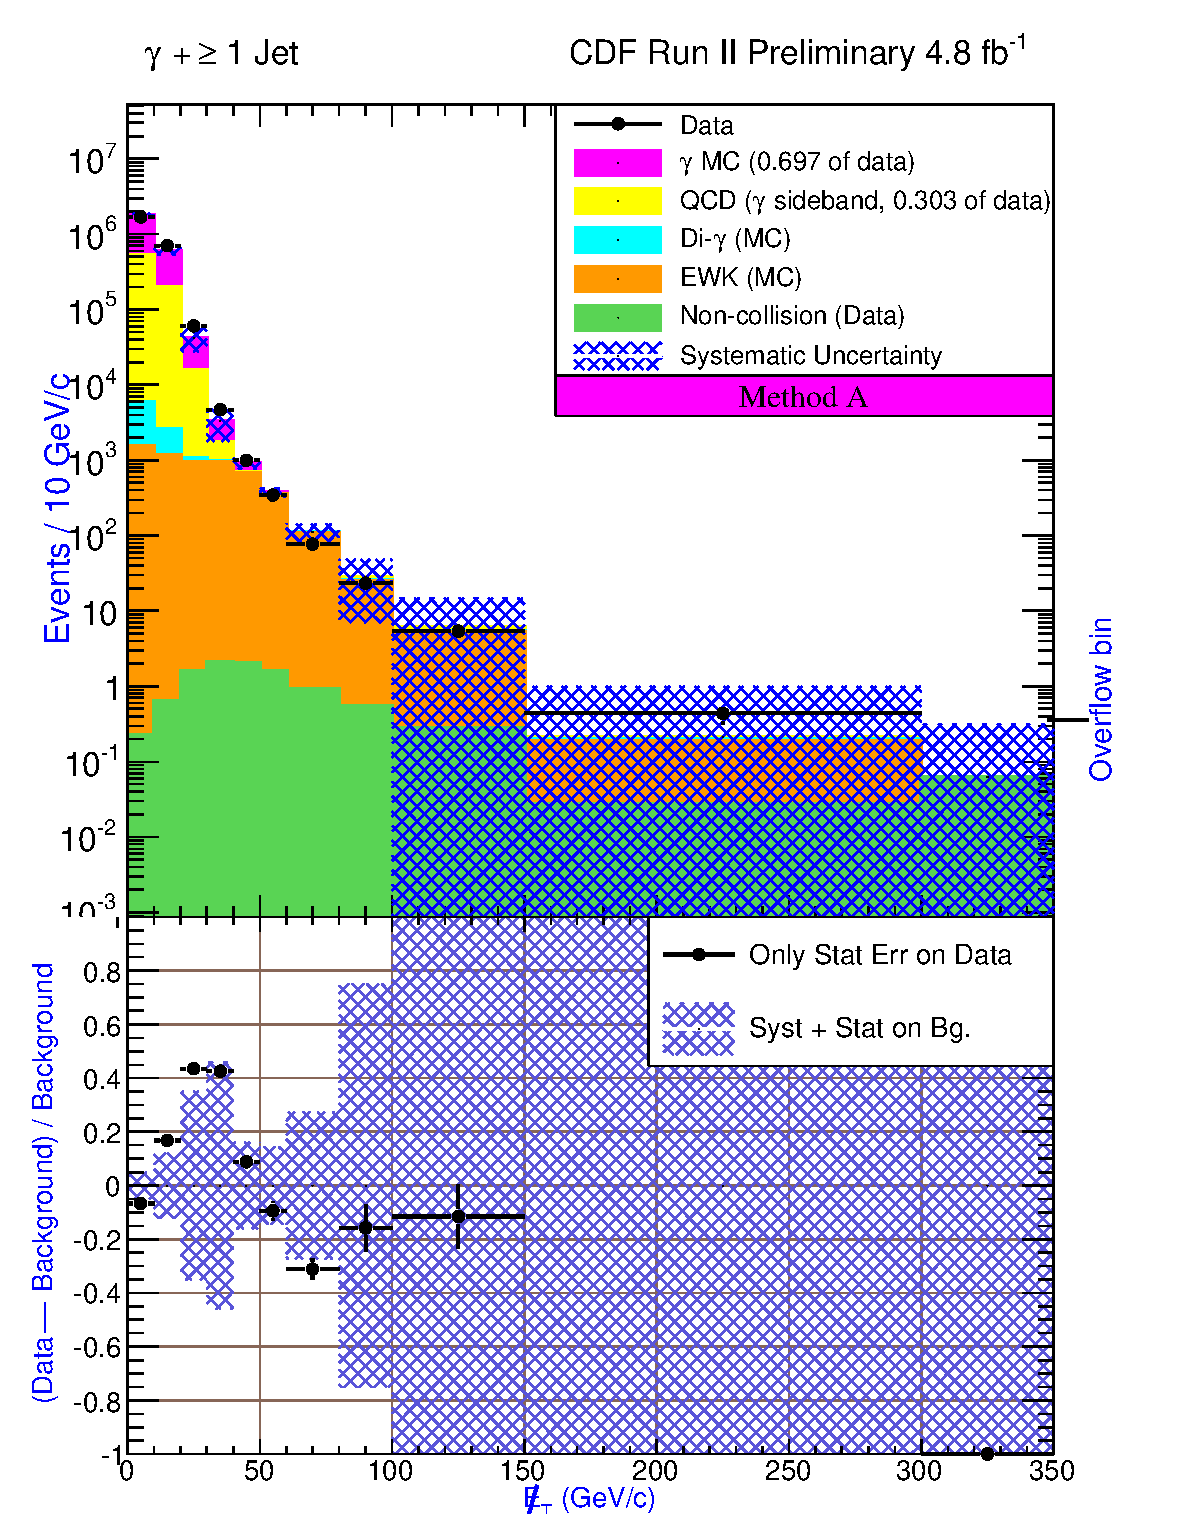
\includegraphics[scale=\resultsHistScale,keepaspectratio=true]{./g30jet_MtdA_plot1_Met.pdf}
 % g30jet_MtdA_plot1_Et_pho.pdf: 567x734 pixel, 72dpi, 20.00x25.89 cm, bb=0 0 567 734
}
\subfigure[]{
 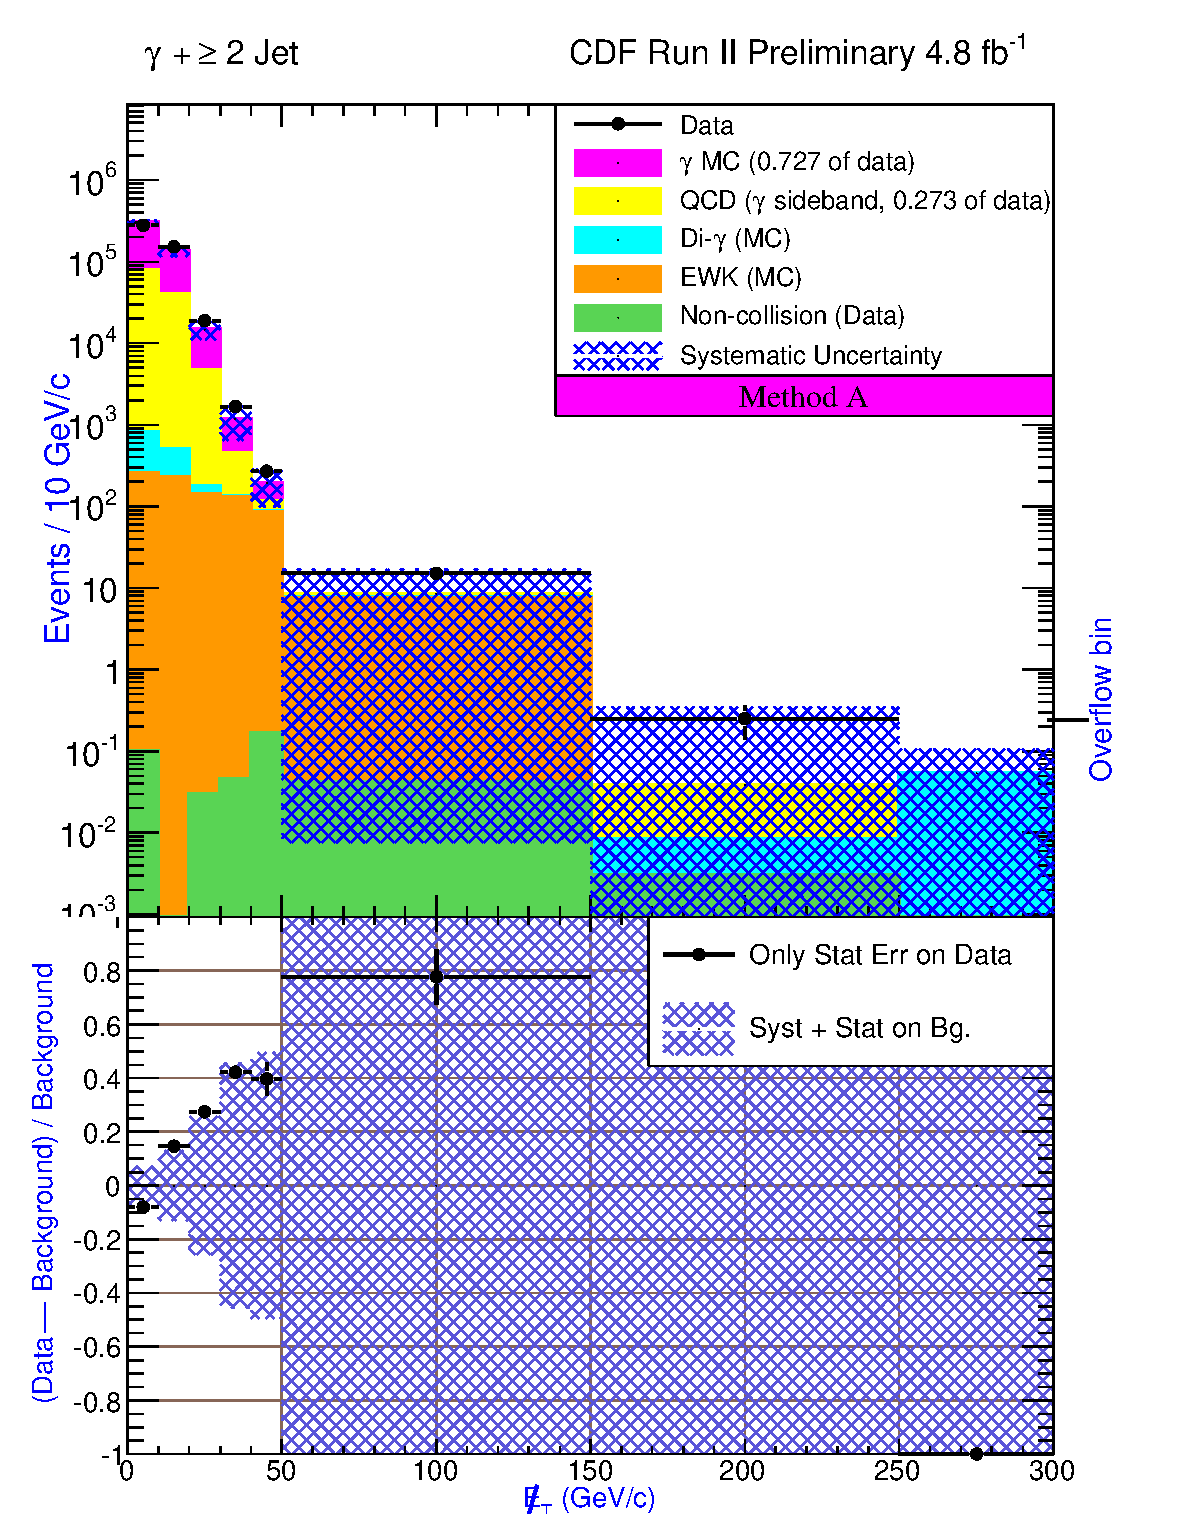
\includegraphics[scale=\resultsHistScale,keepaspectratio=true]{./g30jet_MtdA_plot2_Met.pdf}
 % g30jet_MtdA_plot1_Et_pho.pdf: 567x734 pixel, 72dpi, 20.00x25.89 cm, bb=0 0 567 734
}
 \caption{\newterm{Method A}: \met distribution of the leading jet in \phoonejet (left) and \photwojet (right) data samples.}
 \label{fig:Result_MtdA_gj1_Met}
\end{figure}

\begin{figure}[h!]
 \centering
\subfigure[]{
 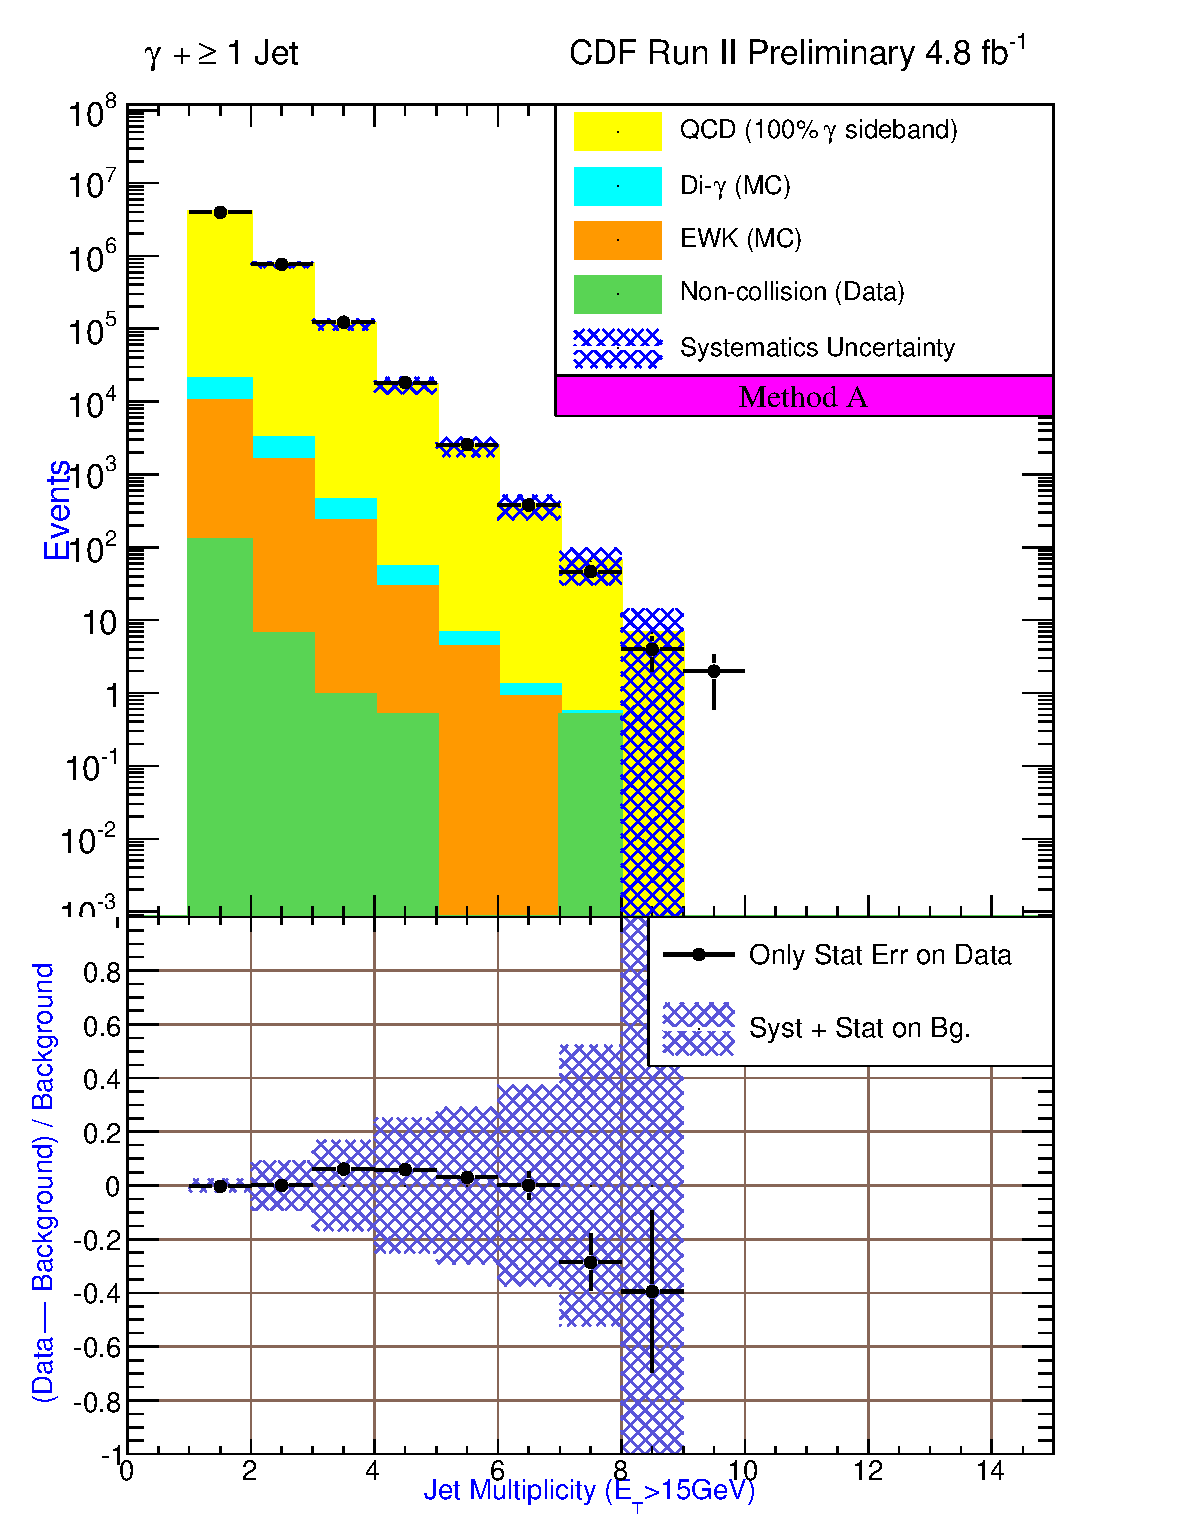
\includegraphics[scale=\resultsHistScale,keepaspectratio=true]{./g30jet_MtdA_plot1_NJet.pdf}
 % g30jet_MtdA_plot1_Et_pho.pdf: 567x734 pixel, 72dpi, 20.00x25.89 cm, bb=0 0 567 734
}
 \caption{\newterm{Method A}: Jet Multiplicity distribution of the leading jet in \phoonejet data sample.}
 \label{fig:Result_MtdA_gj1_Njet}
\end{figure}


\begin{figure}[h!]
 \centering
\subfigure[]{
 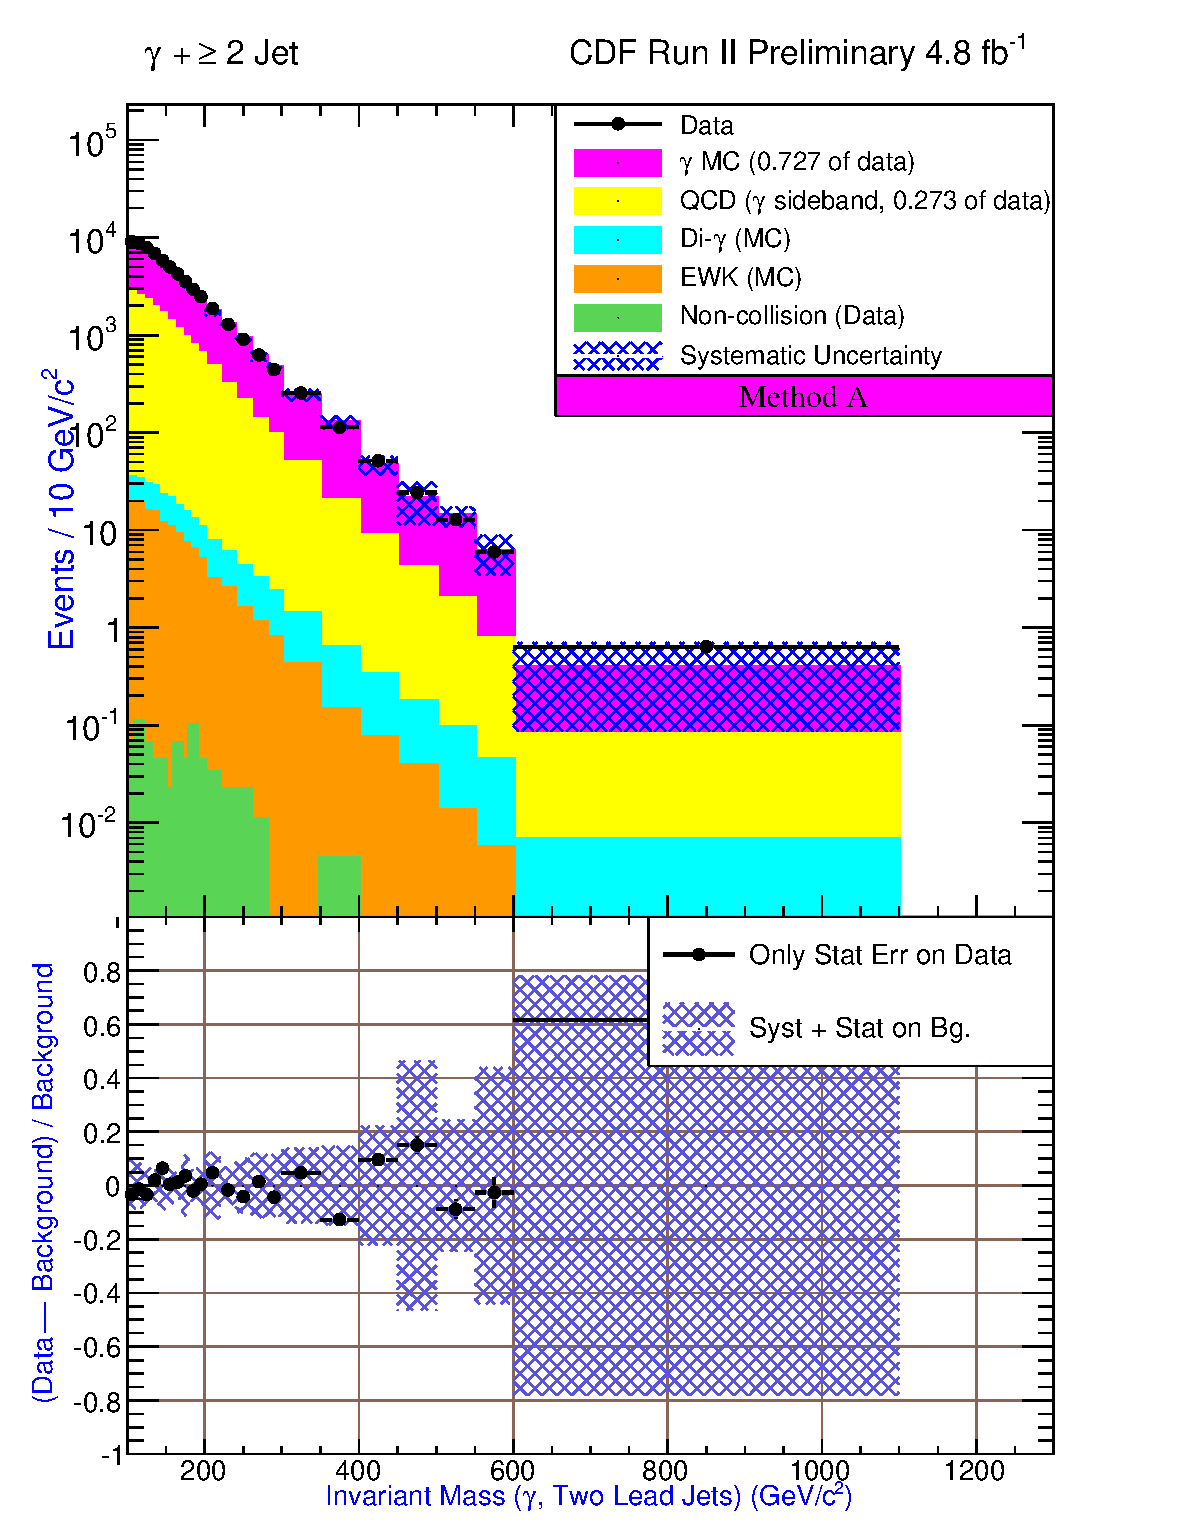
\includegraphics[scale=\resultsHistScale,keepaspectratio=true]{./g30jet_MtdA_plot2_InvMass_pj1j2.pdf}
 % g30jet_MtdA_plot1_Et_pho.pdf: 567x734 pixel, 72dpi, 20.00x25.89 cm, bb=0 0 567 734
}
\subfigure[]{
 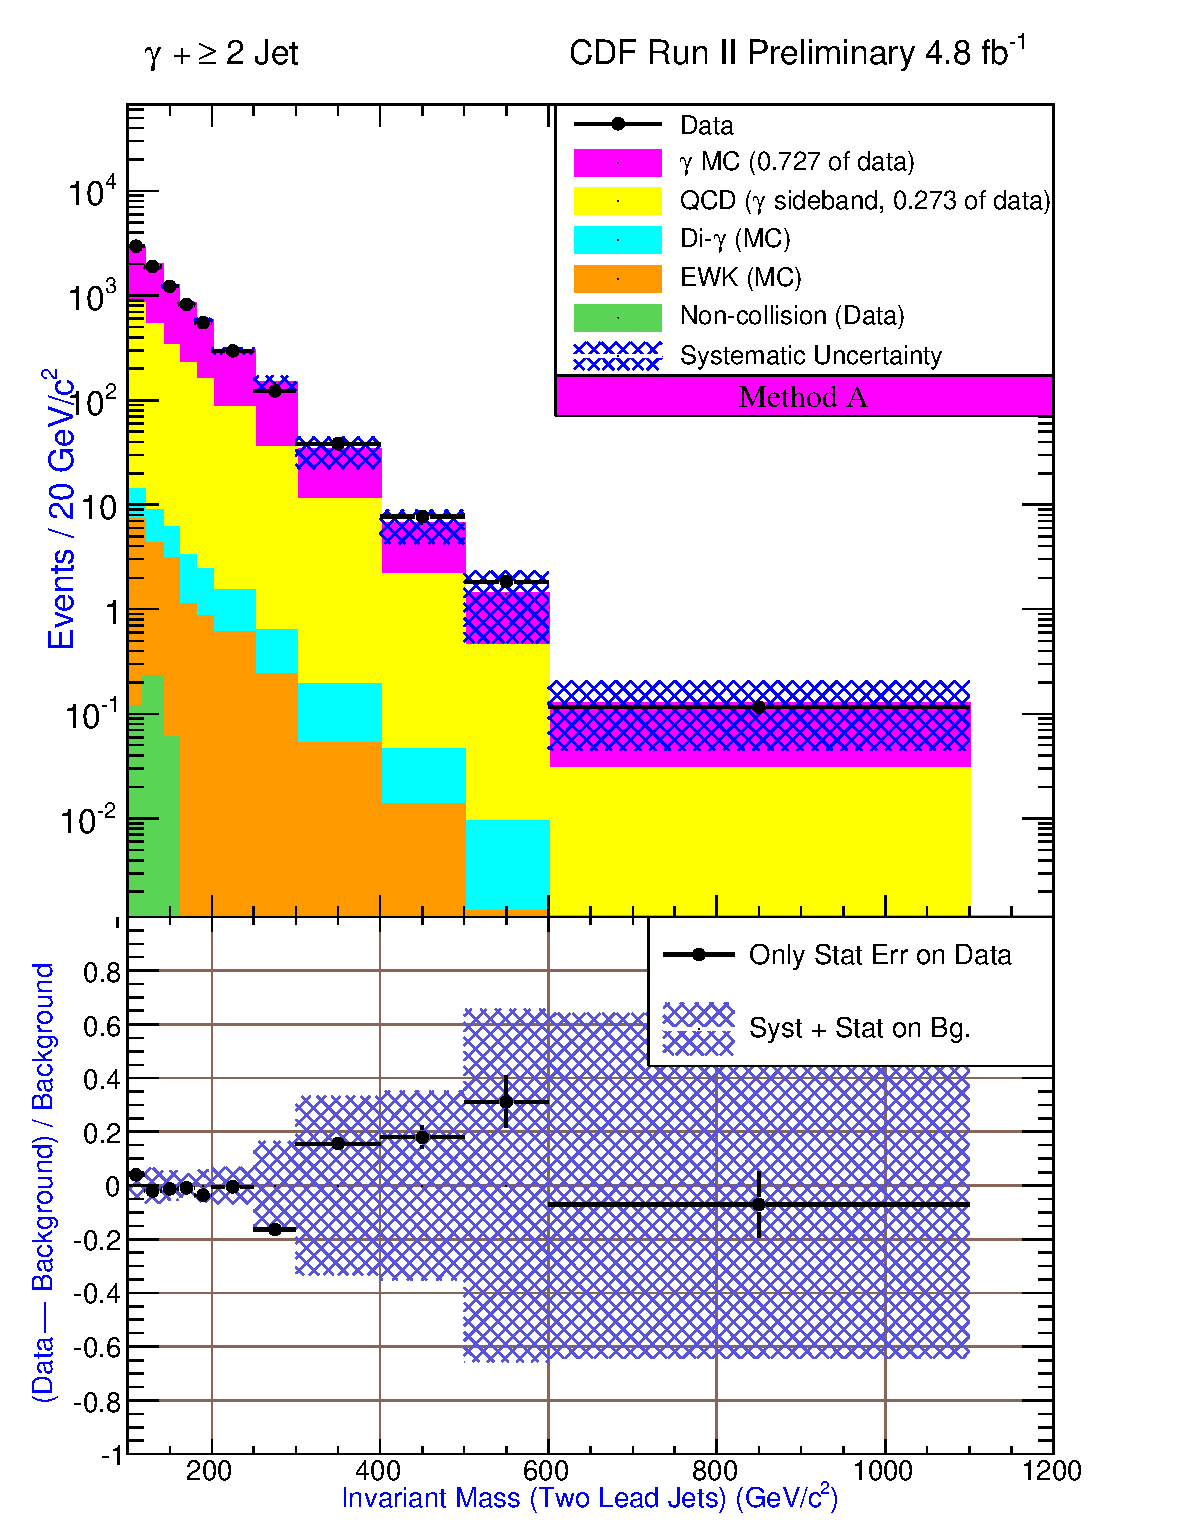
\includegraphics[scale=\resultsHistScale,keepaspectratio=true]{./g30jet_MtdA_plot2_InvMass_j1j2.pdf}
 % g30jet_MtdA_plot1_Et_pho.pdf: 567x734 pixel, 72dpi, 20.00x25.89 cm, bb=0 0 567 734
}
 \caption{\newterm{Method A}: Invariant mass of the photon and the two leading jets (left) and the invariant mass of the two leading jets (right), in \photwojet data sample.}
 \label{fig:Result_MtdA_gj2_Mass_gj1j2}
\end{figure}


%%%%%%%%%%%%%%%%%%%%%%%%%%%%%%%%%%
%%% METHOD B PLOTS:
%%%%%%%%%%%%%%%%%%%%%%%%%%%%%%%%%%
\begin{figure}[h!]
 \centering
\subfigure[]{
 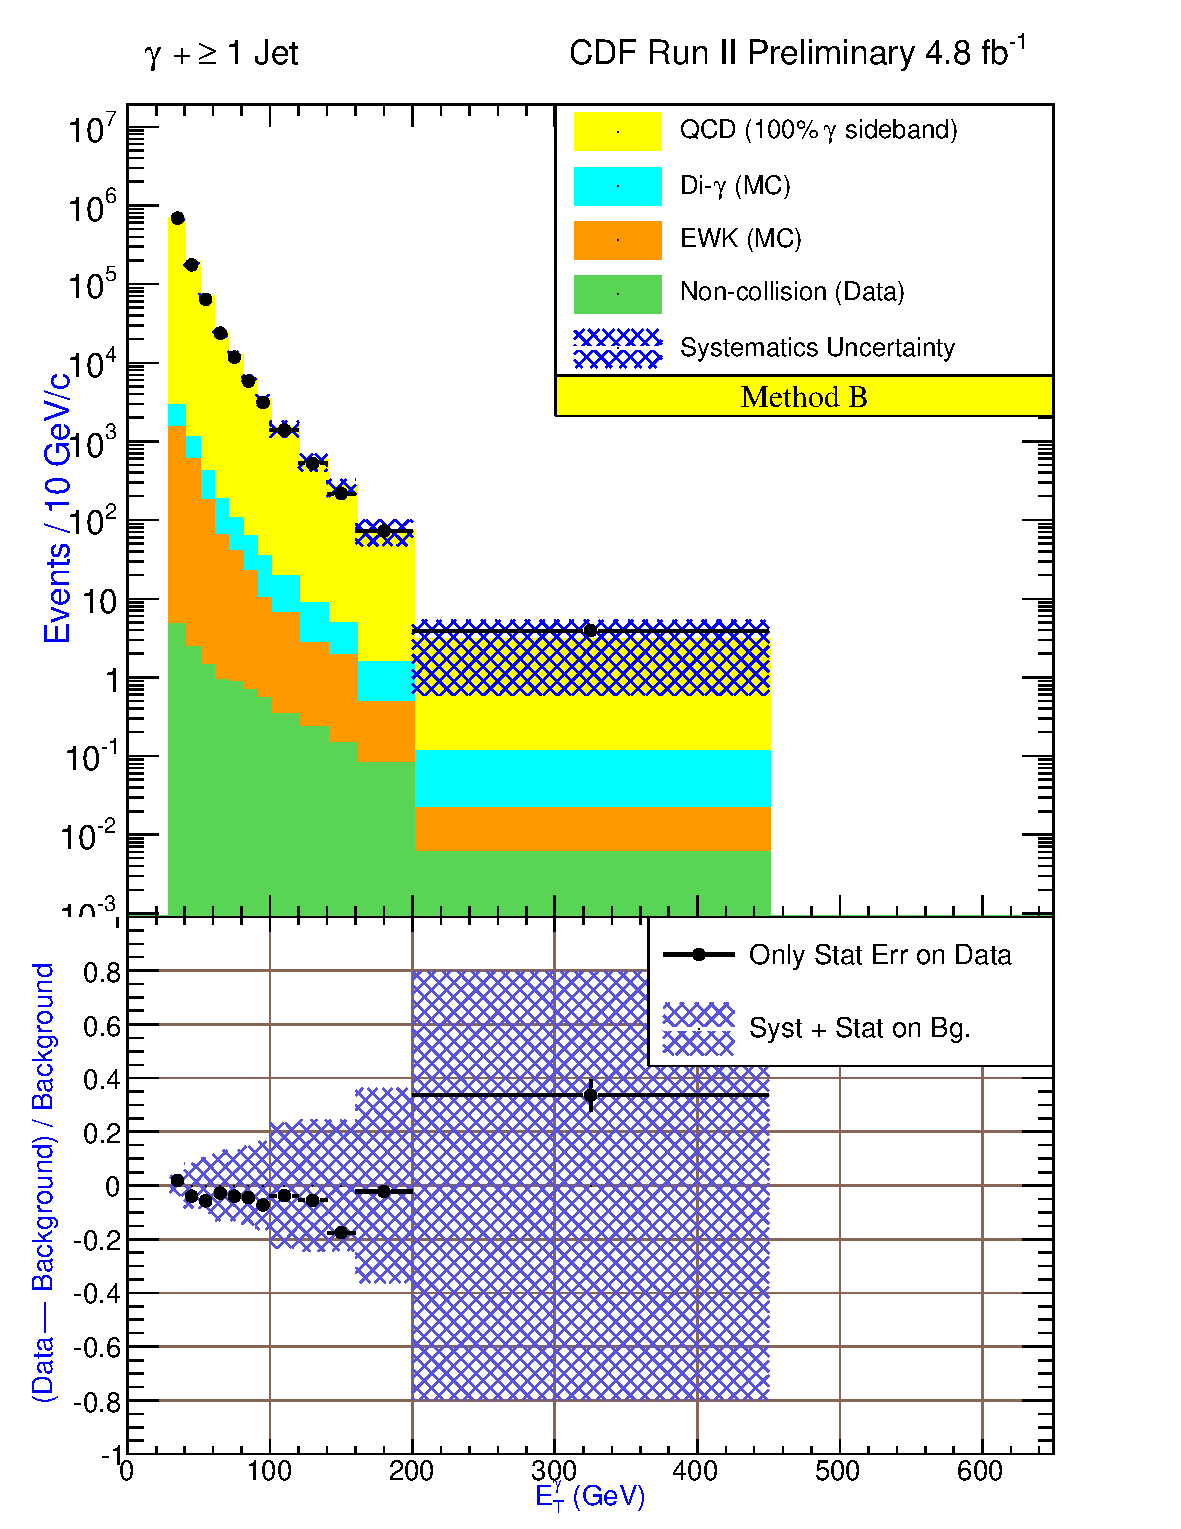
\includegraphics[scale=\resultsHistScale,keepaspectratio=true]{./g30jet_MtdB_plot1_Et_pho.pdf}
 % g30jet_MtdB_plot1_Et_pho.pdf: 567x734 pixel, 72dpi, 20.00x25.89 cm, bb=0 0 567 734
}
\subfigure[]{
 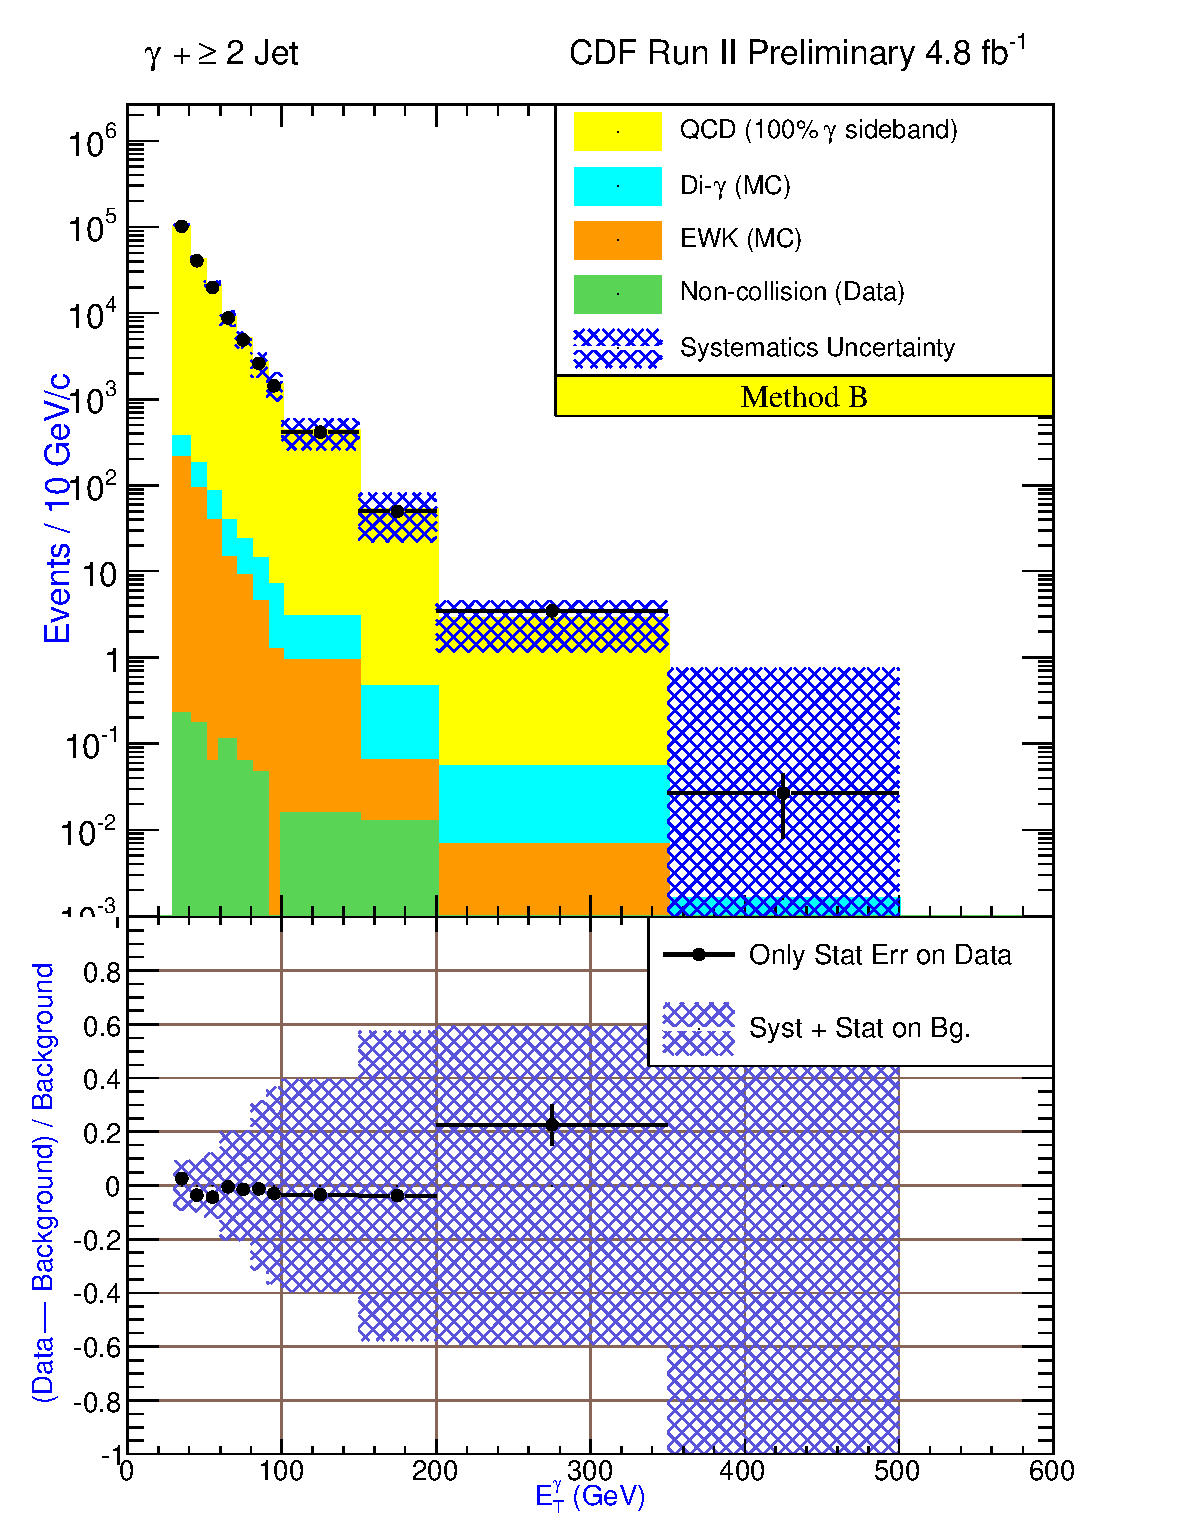
\includegraphics[scale=\resultsHistScale,keepaspectratio=true]{./g30jet_MtdB_plot2_Et_pho.pdf}
 % g30jet_MtdB_plot1_Et_pho.pdf: 567x734 pixel, 72dpi, 20.00x25.89 cm, bb=0 0 567 734
}

 \caption{\newterm{Method B}: Photon \et distribution of the \phoonejet (left) and \photwojet (right) data samples.}
 \label{fig:Result_MtdB_gj1_PhoEt}
\end{figure}

\begin{figure}[h!]
 \centering
\subfigure[]{
 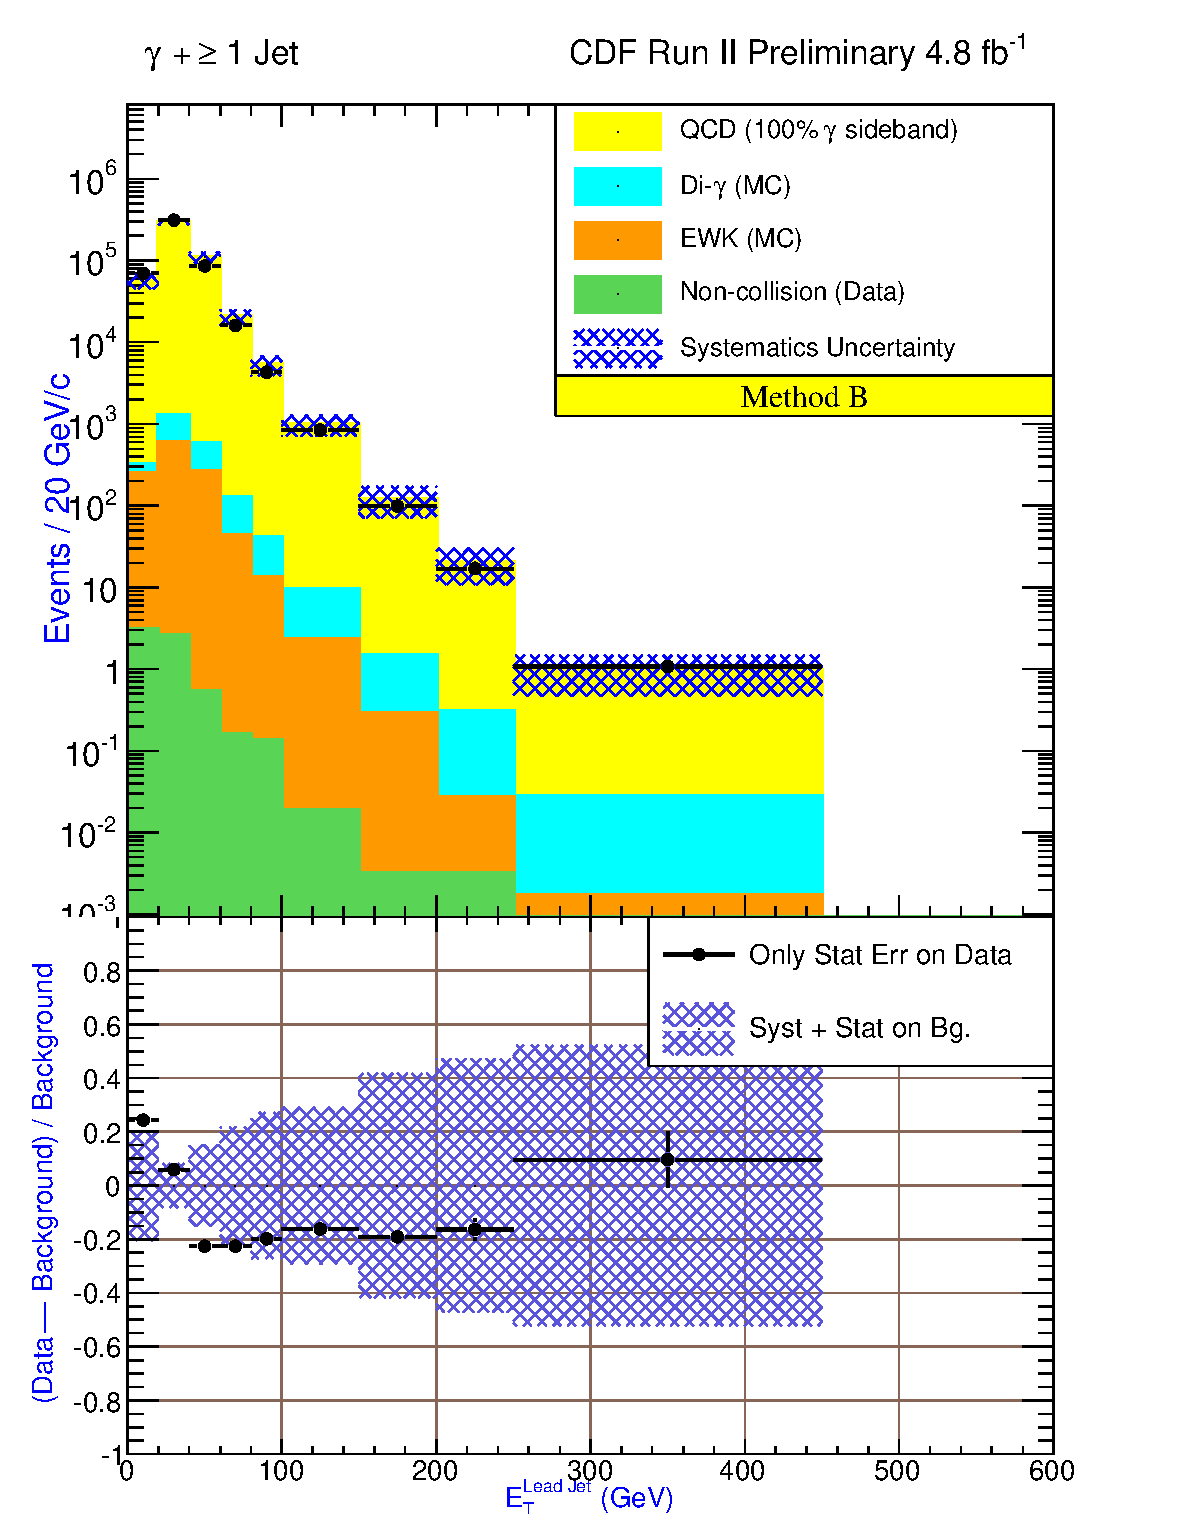
\includegraphics[scale=\resultsHistScale,keepaspectratio=true]{./g30jet_MtdB_plot1_Et_j1.pdf}
 % g30jet_MtdB_plot1_Et_pho.pdf: 567x734 pixel, 72dpi, 20.00x25.89 cm, bb=0 0 567 734
}
\subfigure[]{
 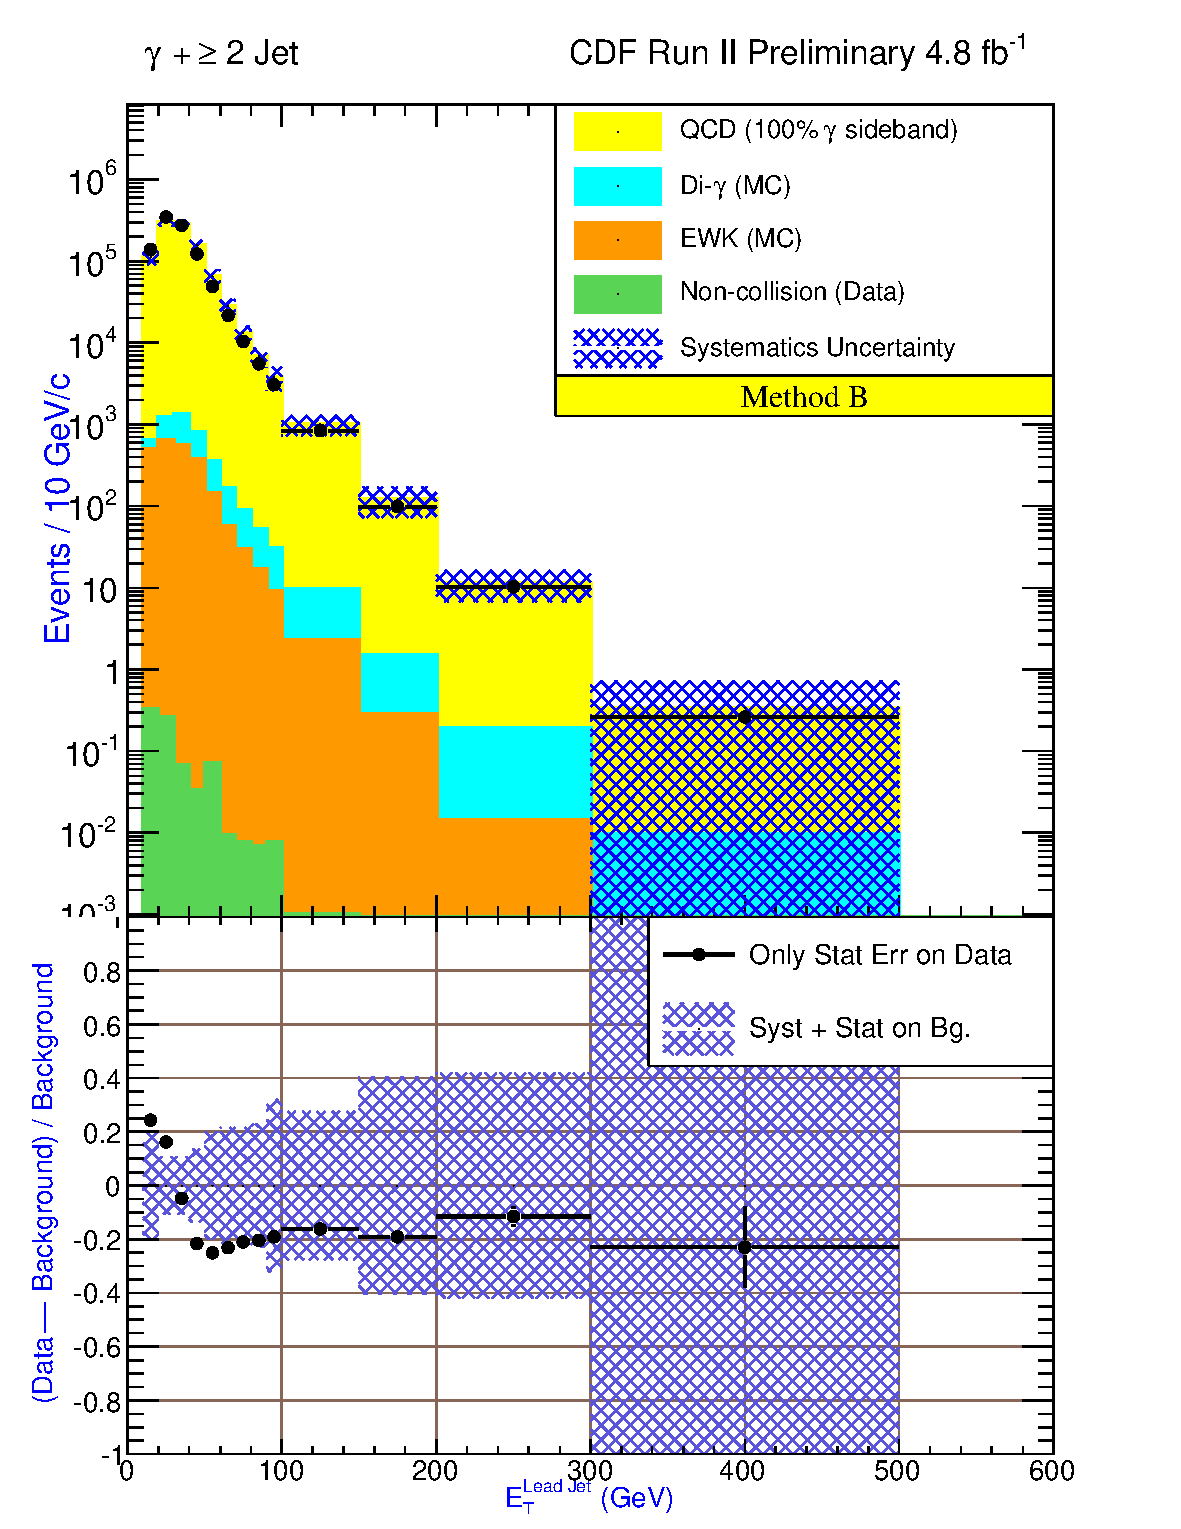
\includegraphics[scale=\resultsHistScale,keepaspectratio=true]{./g30jet_MtdB_plot2_Et_j1.pdf}
 % g30jet_MtdB_plot1_Et_pho.pdf: 567x734 pixel, 72dpi, 20.00x25.89 cm, bb=0 0 567 734
}
 \caption{\newterm{Method B}: \et distribution of the leading jet in \phoonejet (left) and \photwojet (right) data samples.}
 \label{fig:Result_MtdB_gj1_JetEt}
\end{figure}

\begin{figure}[h!]
 \centering
 \subfigure[]{
 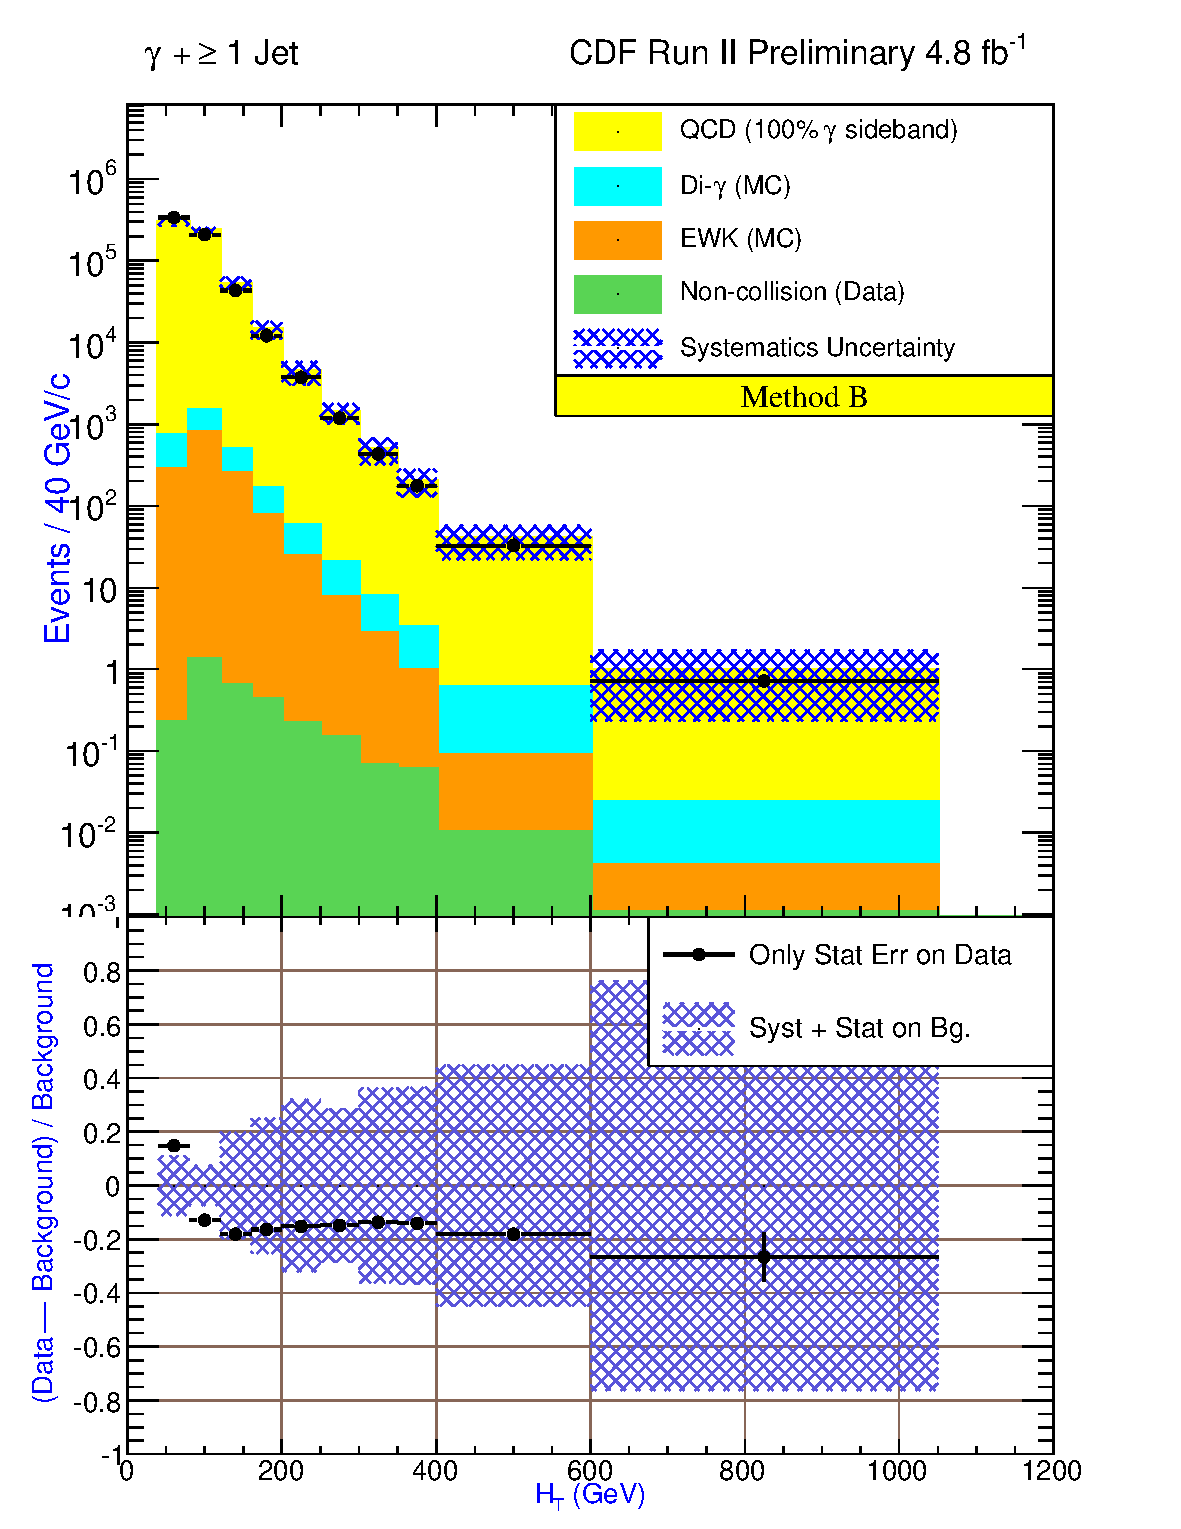
\includegraphics[scale=\resultsHistScale,keepaspectratio=true]{./g30jet_MtdB_plot1_Ht.pdf}
 % g30jet_MtdB_plot1_Et_pho.pdf: 567x734 pixel, 72dpi, 20.00x25.89 cm, bb=0 0 567 734
}
 \subfigure[]{
 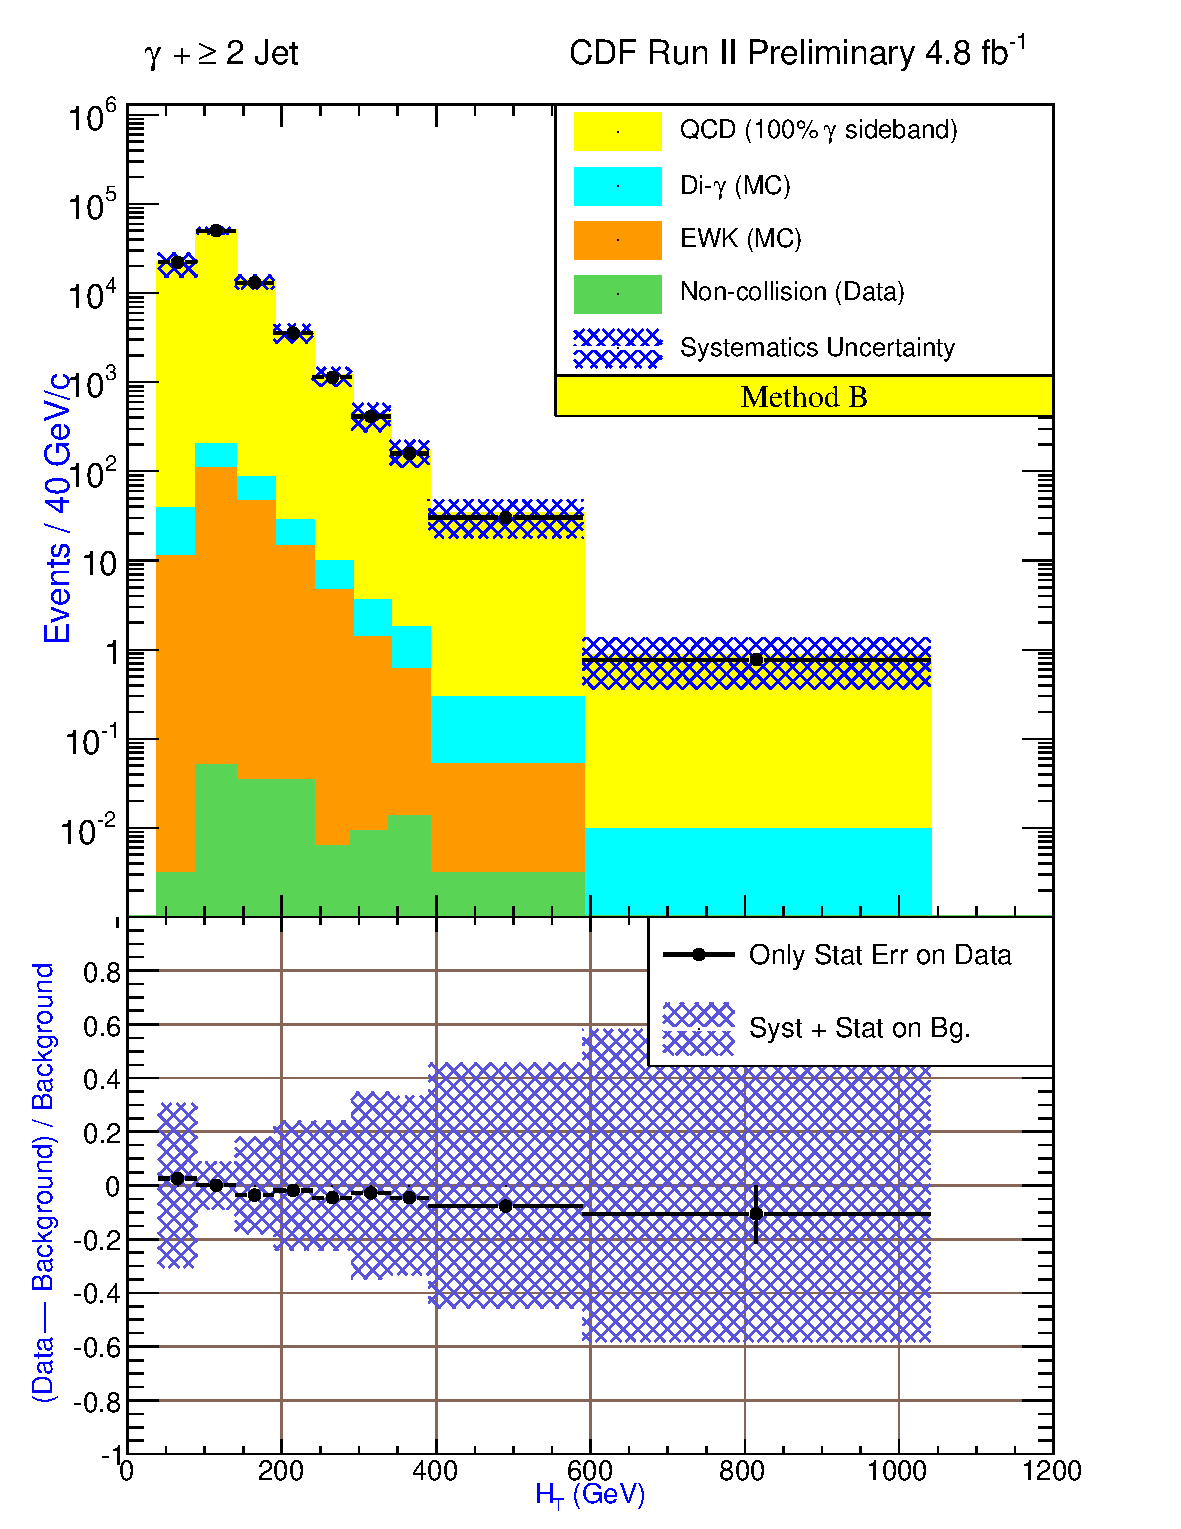
\includegraphics[scale=\resultsHistScale,keepaspectratio=true]{./g30jet_MtdB_plot2_Ht.pdf}
 % g30jet_MtdB_plot1_Et_pho.pdf: 567x734 pixel, 72dpi, 20.00x25.89 cm, bb=0 0 567 734
}
 \caption{\newterm{Method B}: \Ht distribution of the leading jet in \phoonejet (left) and \photwojet (right) data samples.}
 \label{fig:Result_MtdB_gj1_Ht}
\end{figure}

\begin{figure}[h!]
 \centering
\subfigure[]{
 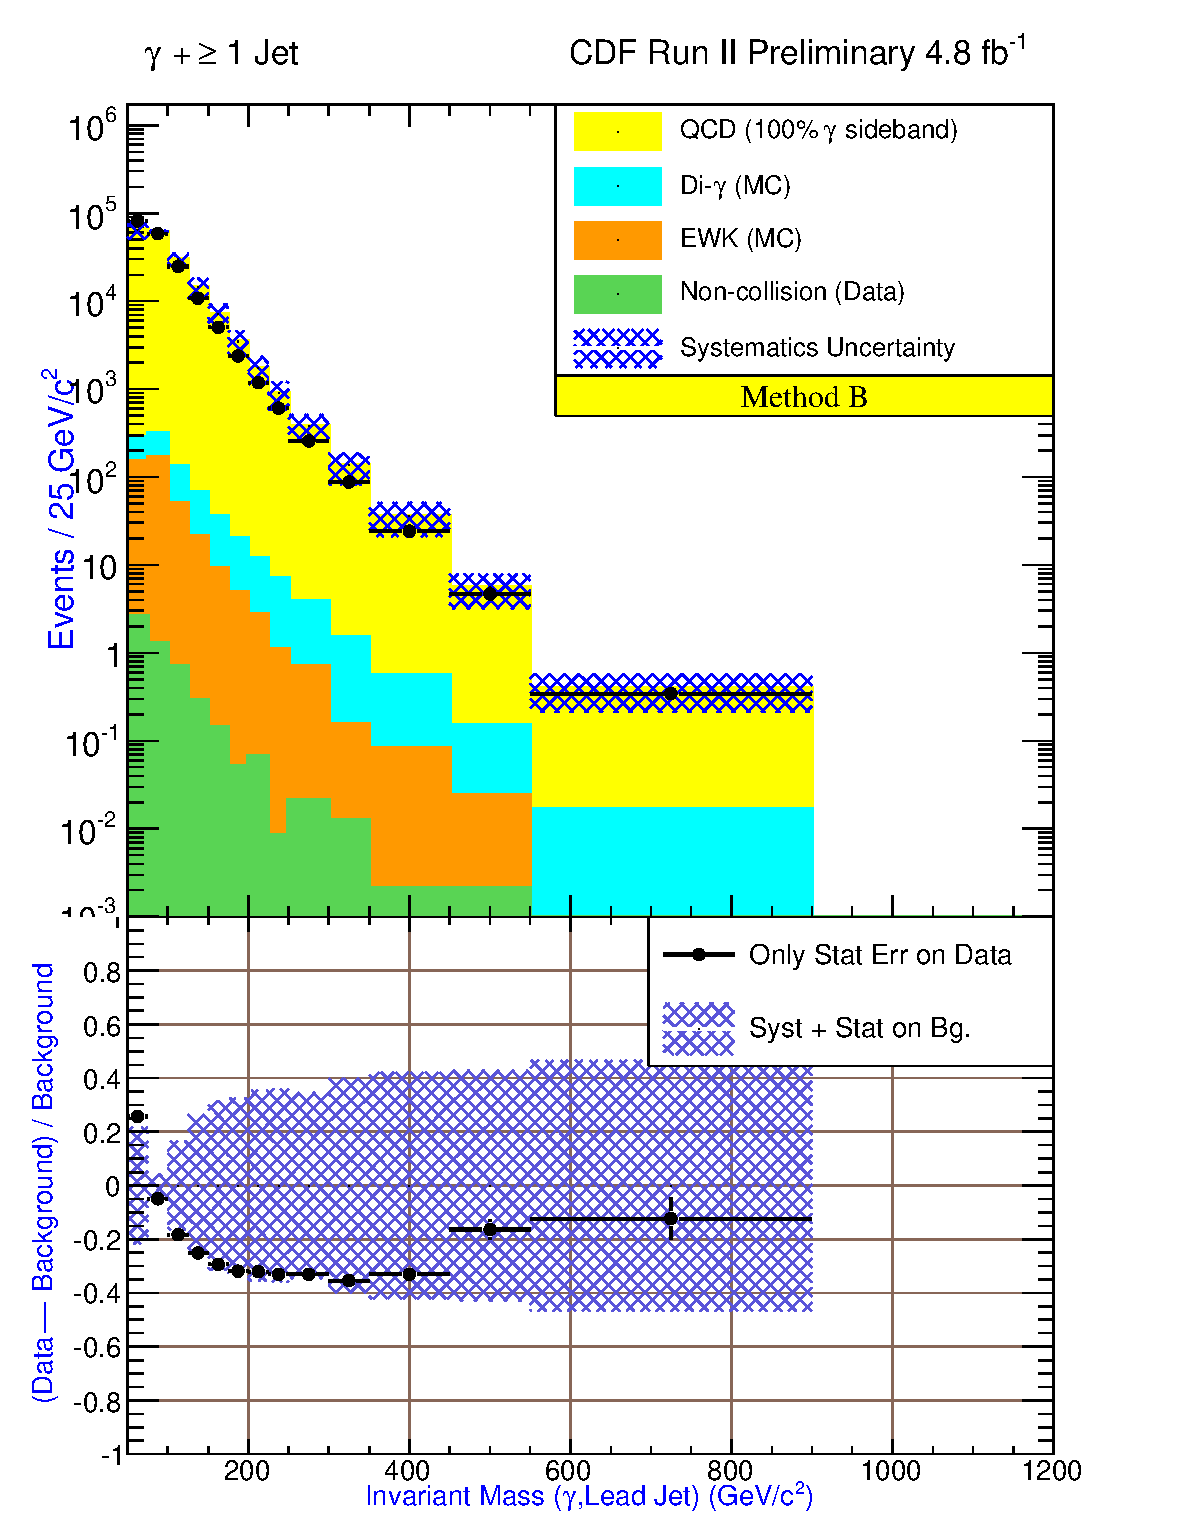
\includegraphics[scale=\resultsHistScale,keepaspectratio=true]{./g30jet_MtdB_plot1_InvMass_pj1.pdf}
 % g30jet_MtdB_plot1_Et_pho.pdf: 567x734 pixel, 72dpi, 20.00x25.89 cm, bb=0 0 567 734
}
\subfigure[]{
 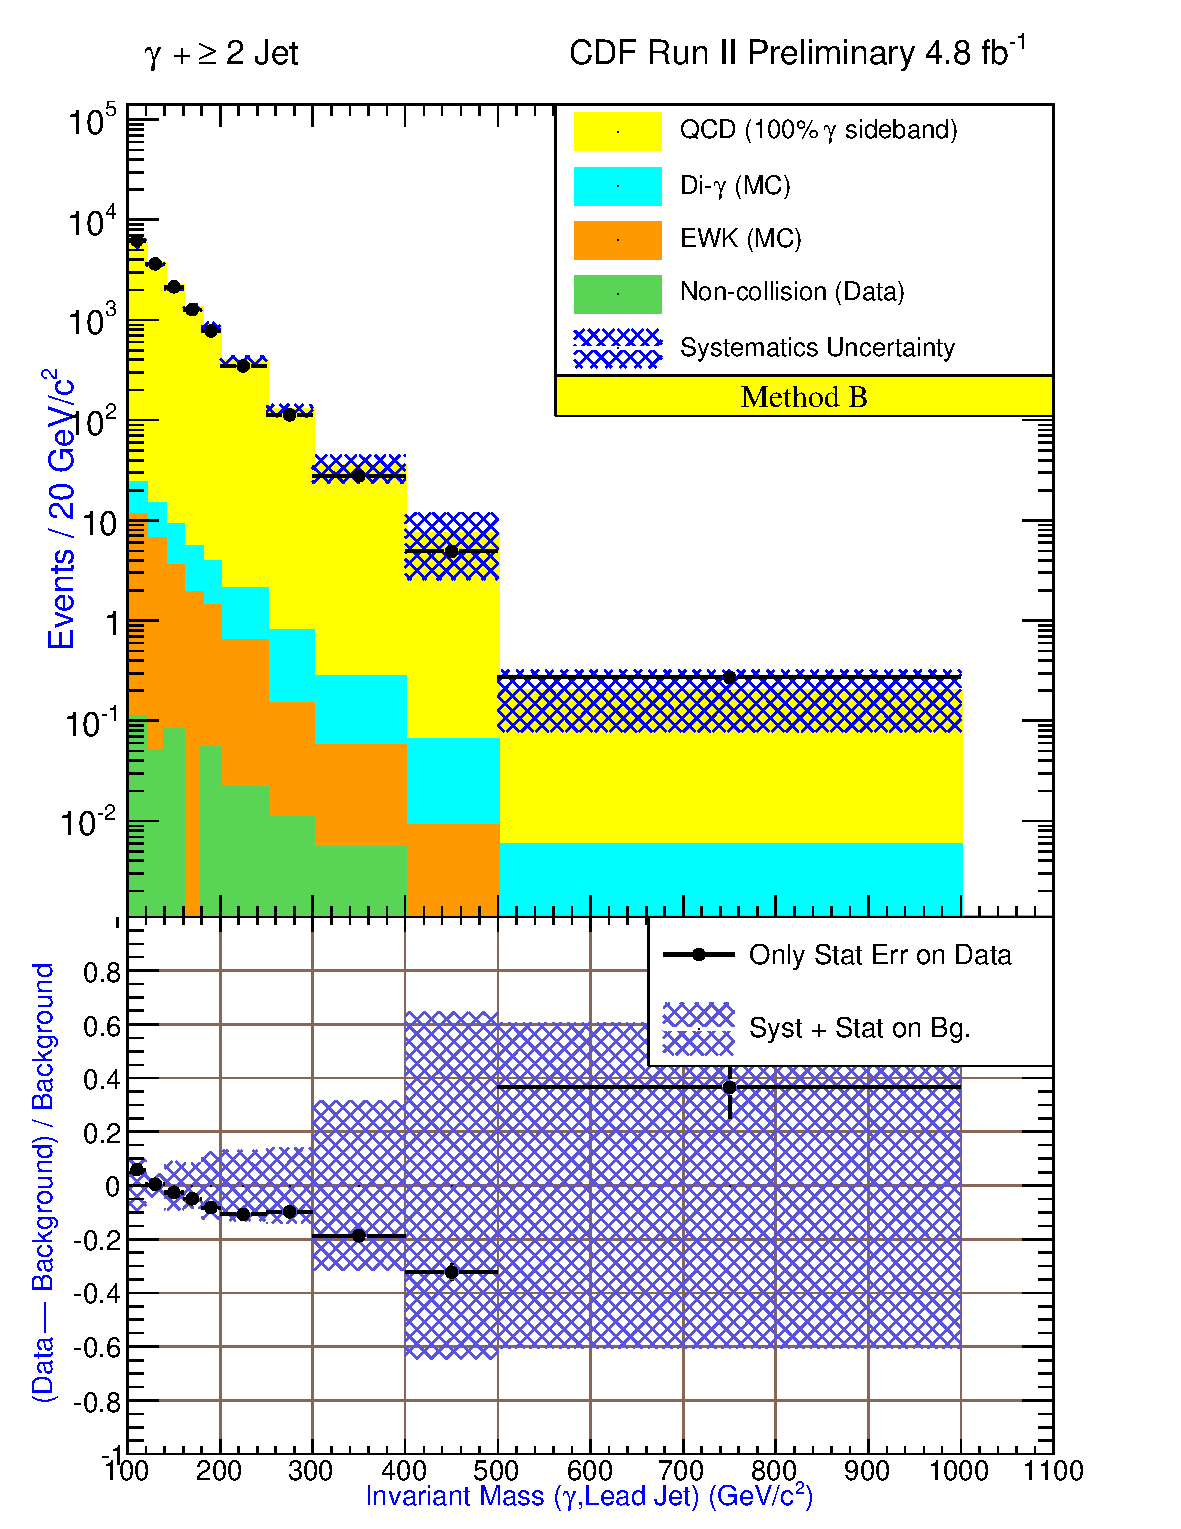
\includegraphics[scale=\resultsHistScale,keepaspectratio=true]{./g30jet_MtdB_plot2_InvMass_pj1.pdf}
 % g30jet_MtdB_plot1_Et_pho.pdf: 567x734 pixel, 72dpi, 20.00x25.89 cm, bb=0 0 567 734
}
 \caption{\newterm{Method B}: Invariant mass of the photon and the leading jet distributions of the leading jet in \phoonejet (left) and \photwojet (right) data samples.}
 \label{fig:Result_MtdB_gj1_Mass_gj1}
\end{figure}

\begin{figure}[h!]
 \centering
\subfigure[]{
 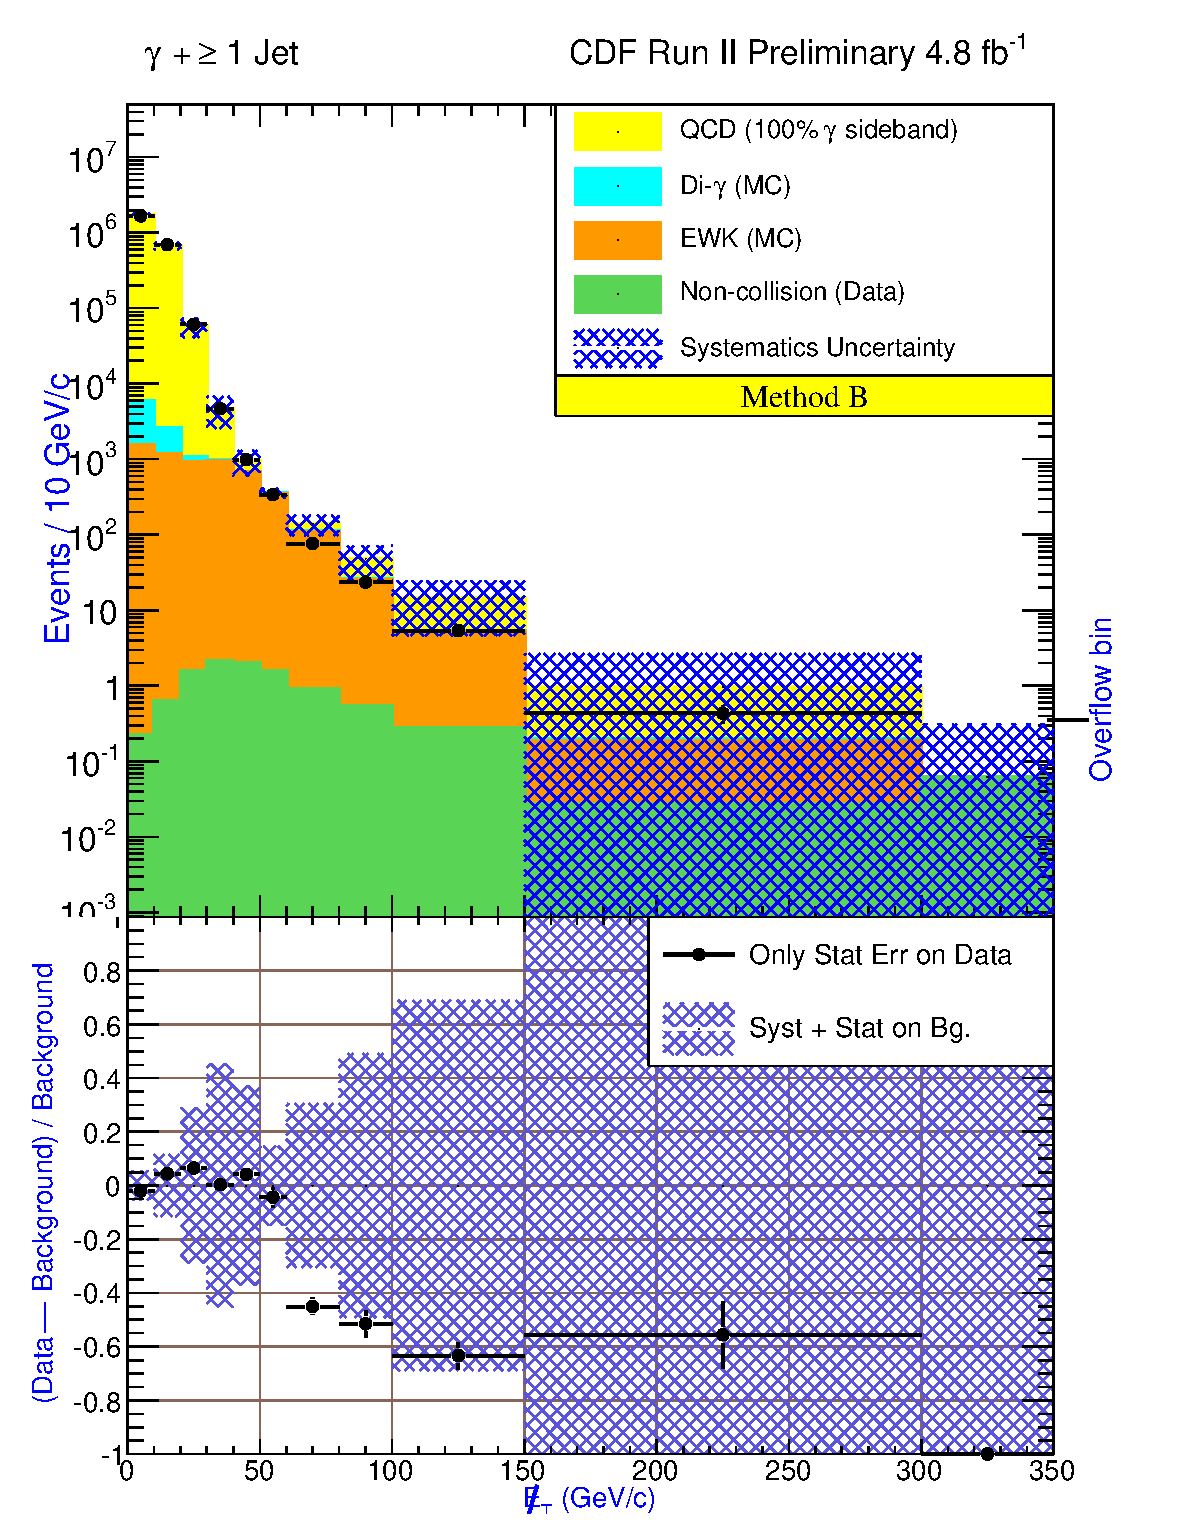
\includegraphics[scale=\resultsHistScale,keepaspectratio=true]{./g30jet_MtdB_plot1_Met.pdf}
 % g30jet_MtdB_plot1_Et_pho.pdf: 567x734 pixel, 72dpi, 20.00x25.89 cm, bb=0 0 567 734
}
\subfigure[]{
 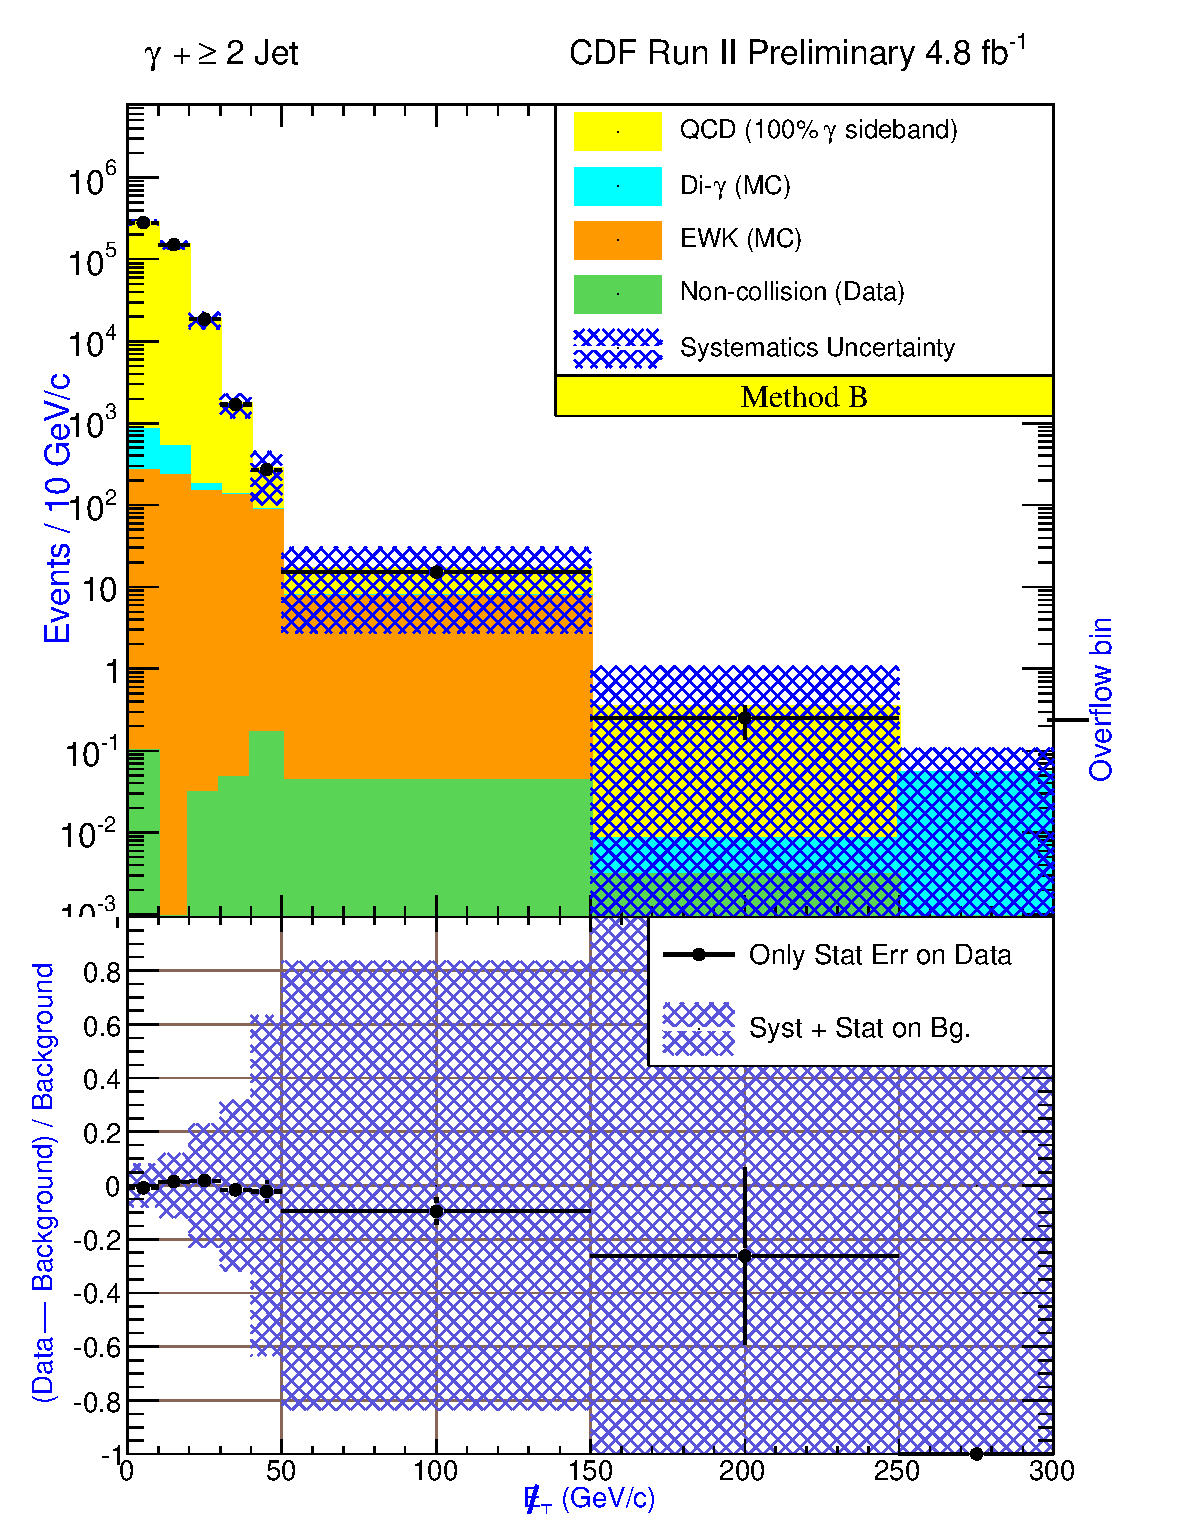
\includegraphics[scale=\resultsHistScale,keepaspectratio=true]{./g30jet_MtdB_plot2_Met.pdf}
 % g30jet_MtdB_plot1_Et_pho.pdf: 567x734 pixel, 72dpi, 20.00x25.89 cm, bb=0 0 567 734
}
 \caption{\newterm{Method B}: \met distribution of the leading jet in \phoonejet (left) and \photwojet (right) data samples.}
 \label{fig:Result_MtdB_gj1_Met}
\end{figure}

\begin{figure}[h!]
 \centering
\subfigure[]{
 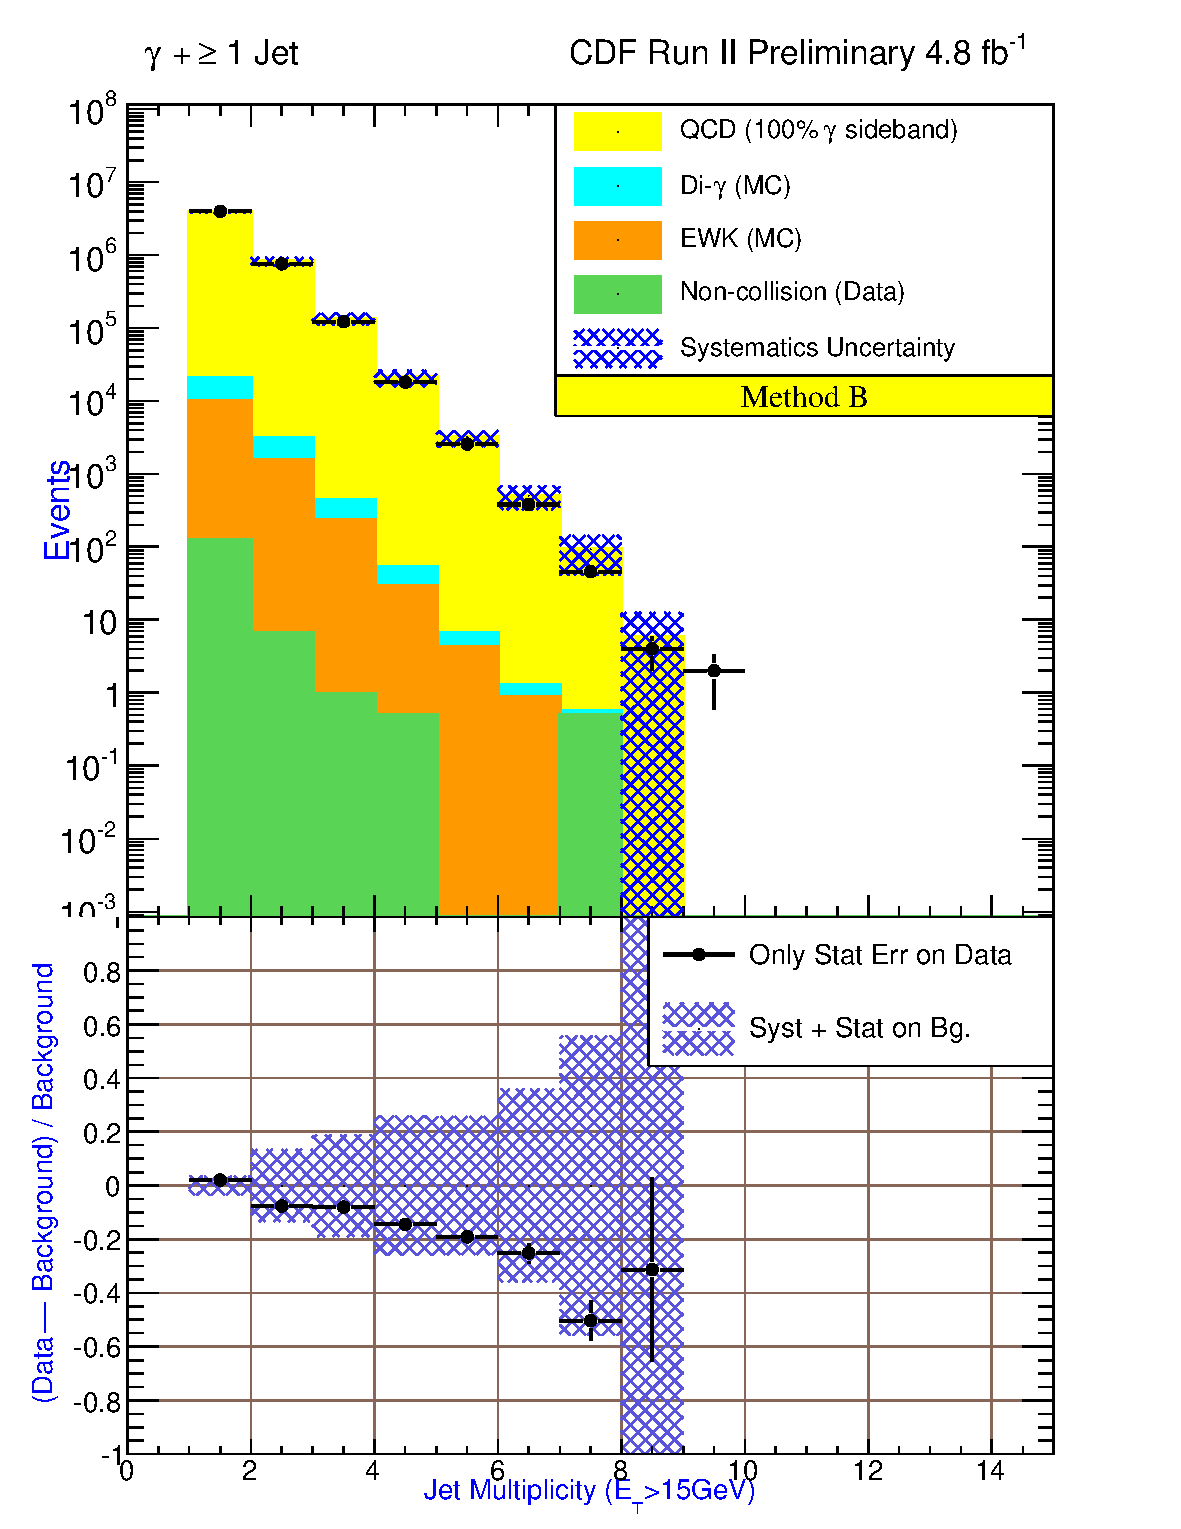
\includegraphics[scale=\resultsHistScale,keepaspectratio=true]{./g30jet_MtdB_plot1_NJet.pdf}
  %g30jet_MtdB_plot1_Et_pho.pdf: 567x734 pixel, 72dpi, 20.00x25.89 cm, bb=0 0 567 734
}
 \caption{\newterm{Method B}: Jet Multiplicity distribution of the leading jet in \phoonejet data sample.}
 \label{fig:Result_MtdB_gj1_Njet}
\end{figure}


\begin{figure}[h!]
 \centering
\subfigure[]{
 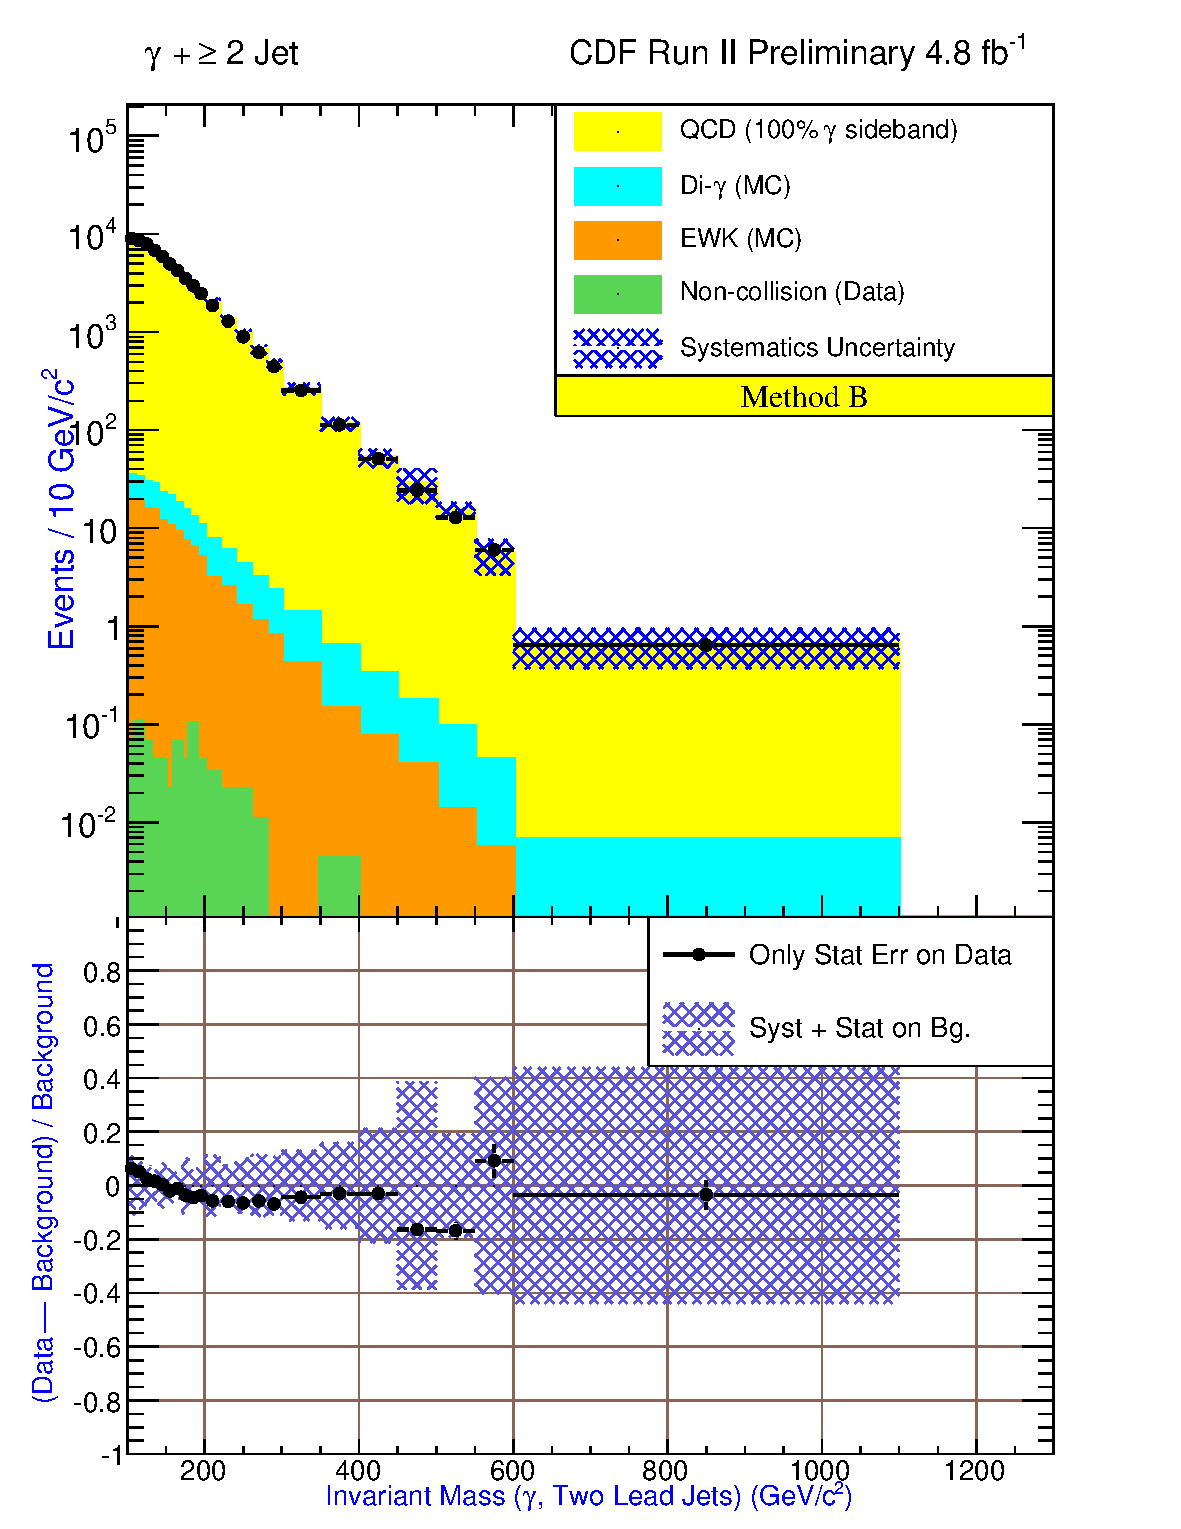
\includegraphics[scale=\resultsHistScale,keepaspectratio=true]{./g30jet_MtdB_plot2_InvMass_pj1j2.pdf}
 % g30jet_MtdB_plot1_Et_pho.pdf: 567x734 pixel, 72dpi, 20.00x25.89 cm, bb=0 0 567 734
}
\subfigure[]{
 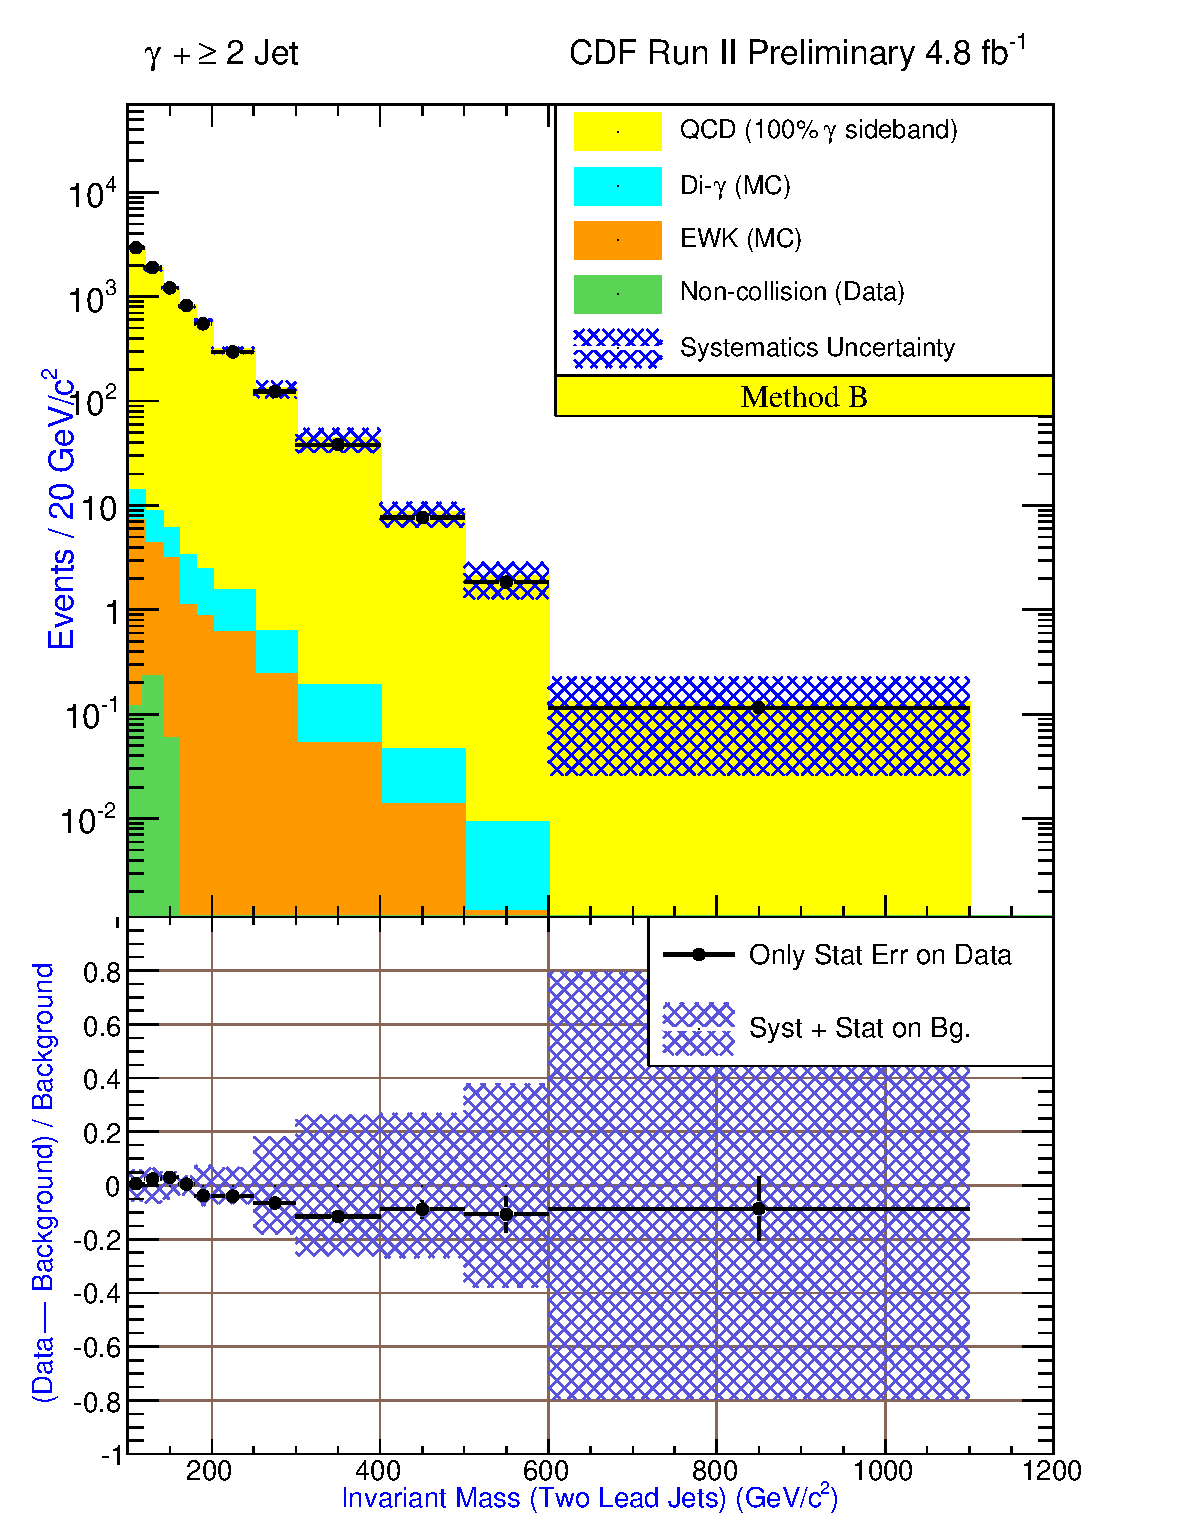
\includegraphics[scale=\resultsHistScale,keepaspectratio=true]{./g30jet_MtdB_plot2_InvMass_j1j2.pdf}
 % g30jet_MtdB_plot1_Et_pho.pdf: 567x734 pixel, 72dpi, 20.00x25.89 cm, bb=0 0 567 734
}
\caption{\newterm{Method B}: Invariant mass of the photon and the two leading jets (left) and the invariant mass of the two leading jets (right), in \photwojet data sample.}
\label{fig:Result_MtdB_gj2_Mass_gj1j2}
\end{figure}

\clearpage
\newpage

%%%%%%%%%%%%%%%%%%%%%%%%%%%%%%%%%%%%%%%%%%%%%%%%%%%%%%%%%%%%%%%%%%%%%%%%%%%%%%%%%%
%\section{$\gamma$+jets+\metCorr$>20$~GeV Kinematic Distributions.}
%%%%%%%%%%%%%%%%%%%%%%%%%%%%%%%%%%%%%%%%%%%%%%%%%%%%%%%%%%%%%%%%%%%%%%%%%%%%%%%%%%

\begin{figure}[h!]
 \centering
\subfigure[]{
 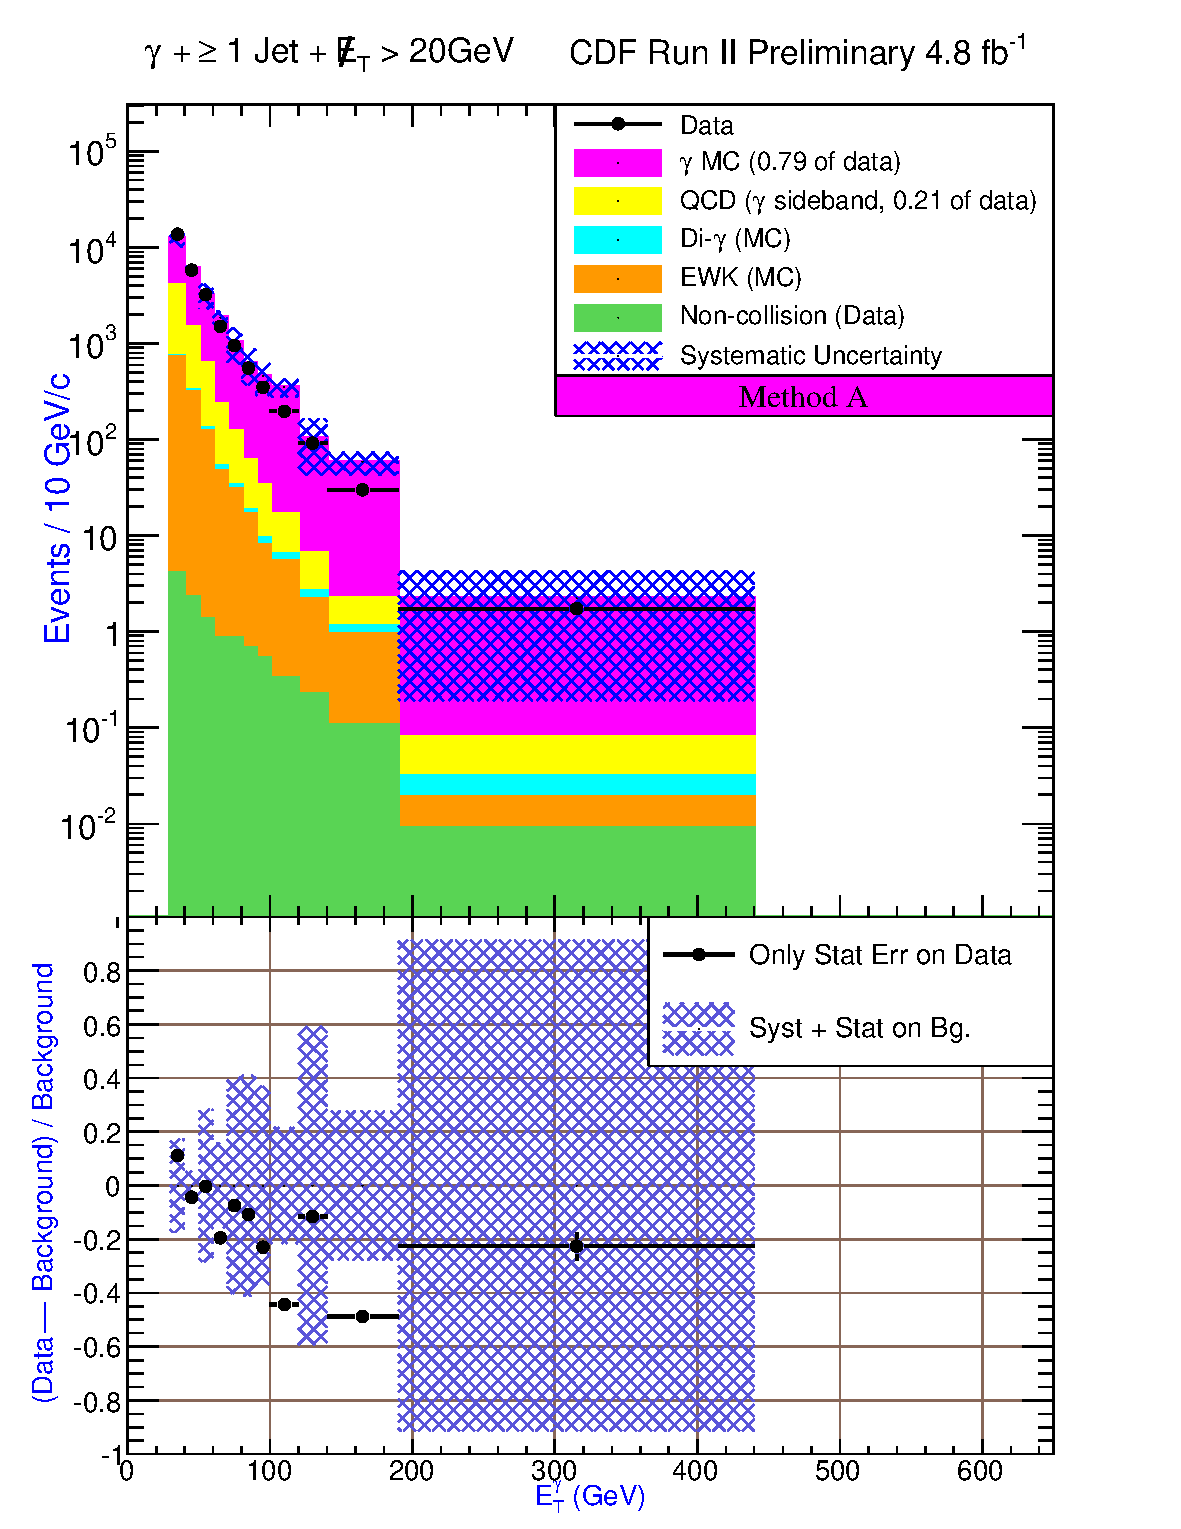
\includegraphics[scale=\resultsHistScale,keepaspectratio=true]{./g30jetmet20_MtdA_plot1_Et_pho.pdf}
 % g30jet_MtdA_plot1_Et_pho.pdf: 567x734 pixel, 72dpi, 20.00x25.89 cm, bb=0 0 567 734
}
\subfigure[]{
 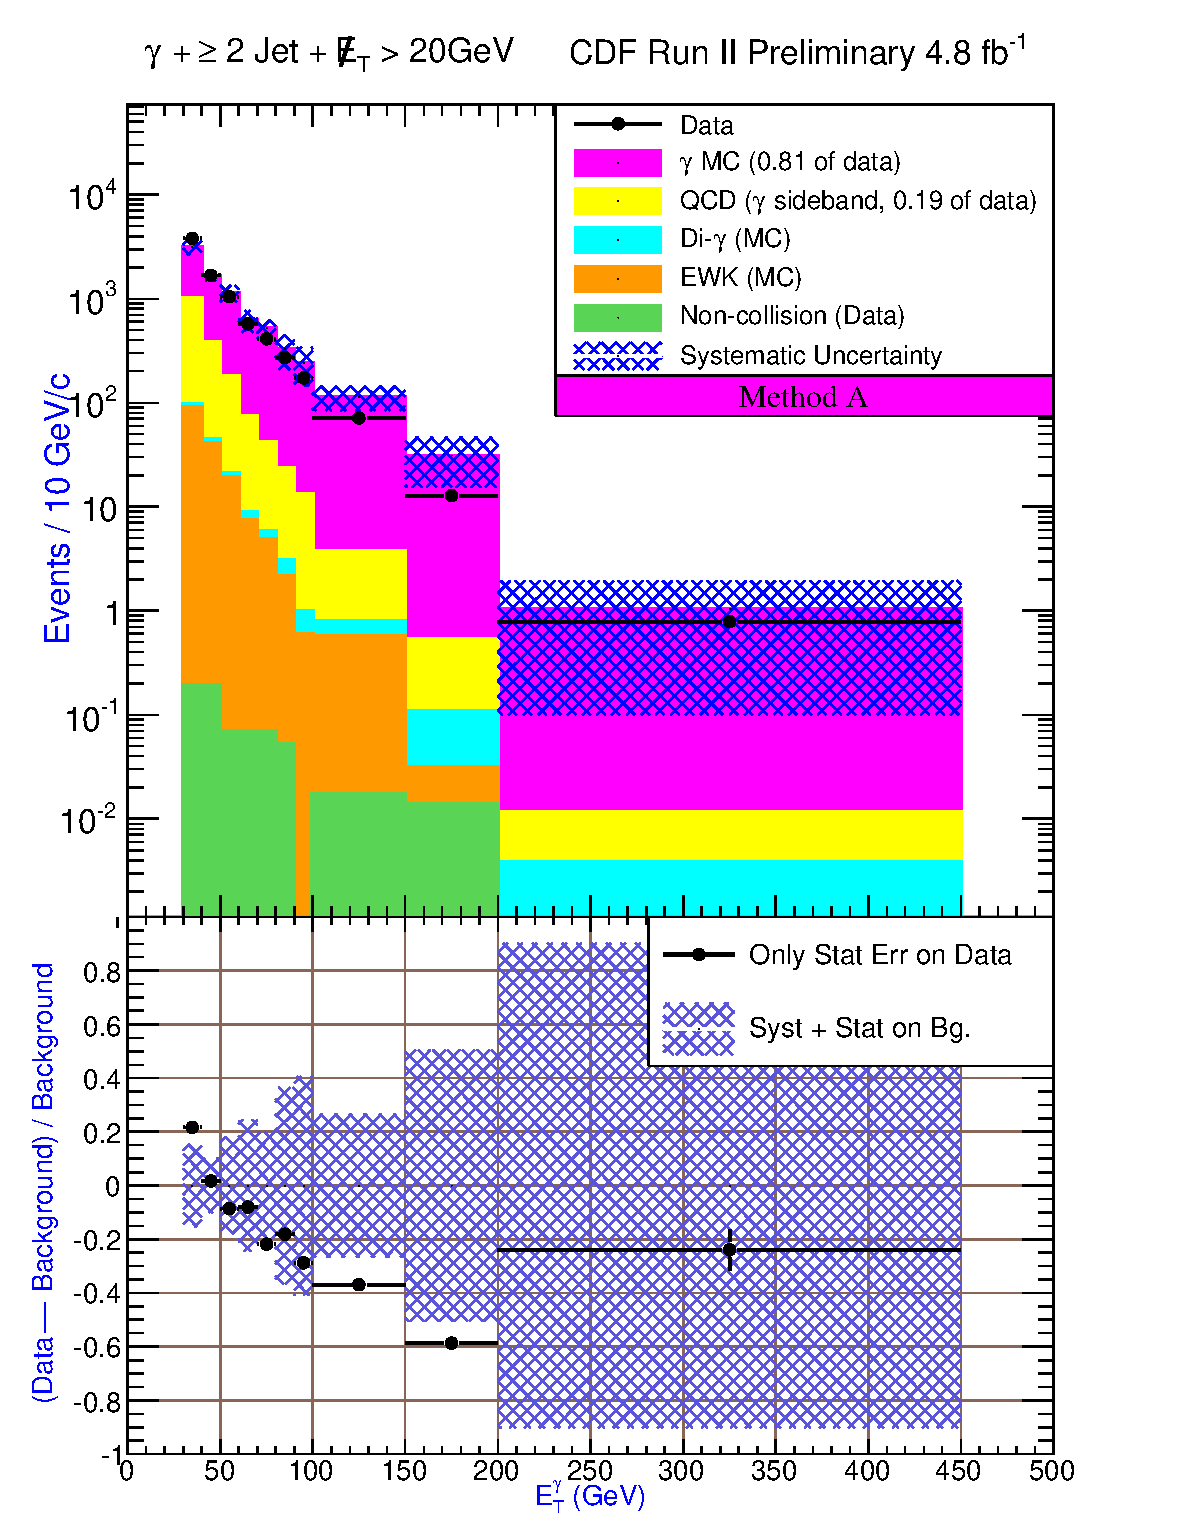
\includegraphics[scale=\resultsHistScale,keepaspectratio=true]{./g30jetmet20_MtdA_plot2_Et_pho.pdf}
 % g30jet_MtdA_plot1_Et_pho.pdf: 567x734 pixel, 72dpi, 20.00x25.89 cm, bb=0 0 567 734
}

 \caption{\newterm{Method A}: Photon \et distribution of the \phoonejetmettwenty (left) and \photwojetmettwenty (right) data samples.}
 \label{fig:Result_MtdA_gj1Met20_PhoEt}
\end{figure}

\begin{figure}[h!]
 \centering
\subfigure[]{
 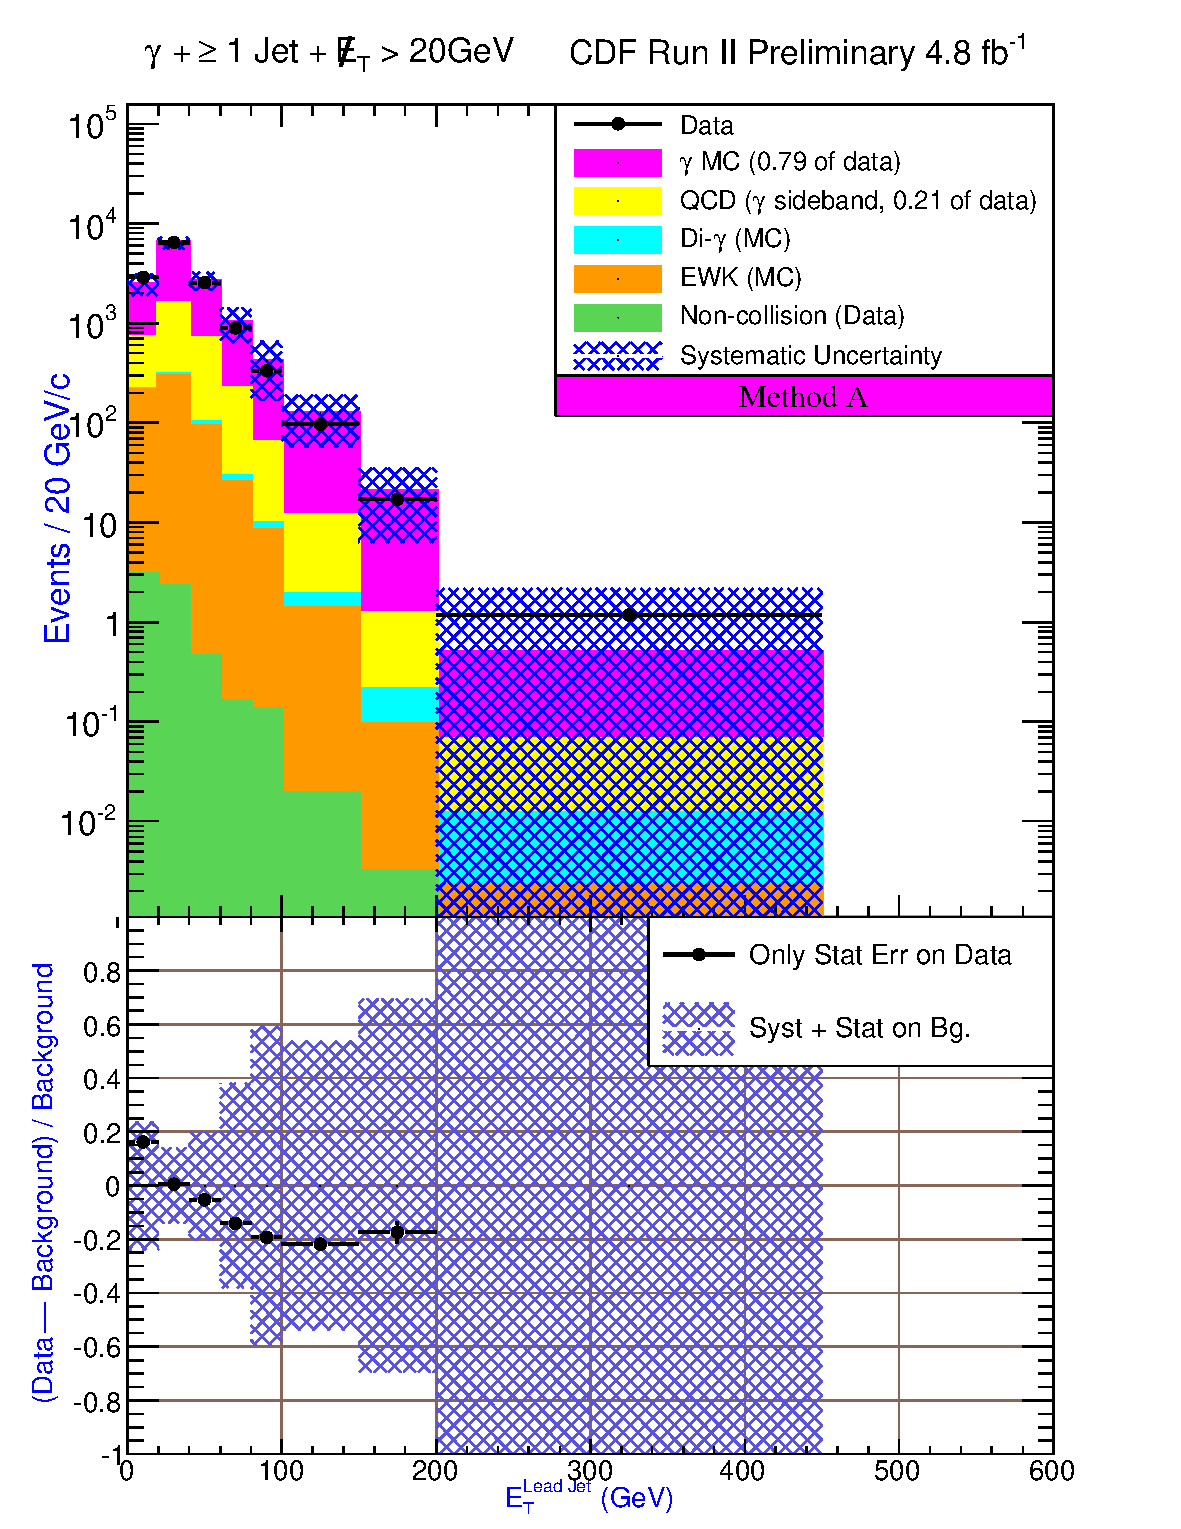
\includegraphics[scale=\resultsHistScale,keepaspectratio=true]{./g30jetmet20_MtdA_plot1_Et_j1.pdf}
 % g30jet_MtdA_plot1_Et_pho.pdf: 567x734 pixel, 72dpi, 20.00x25.89 cm, bb=0 0 567 734
}
\subfigure[]{
 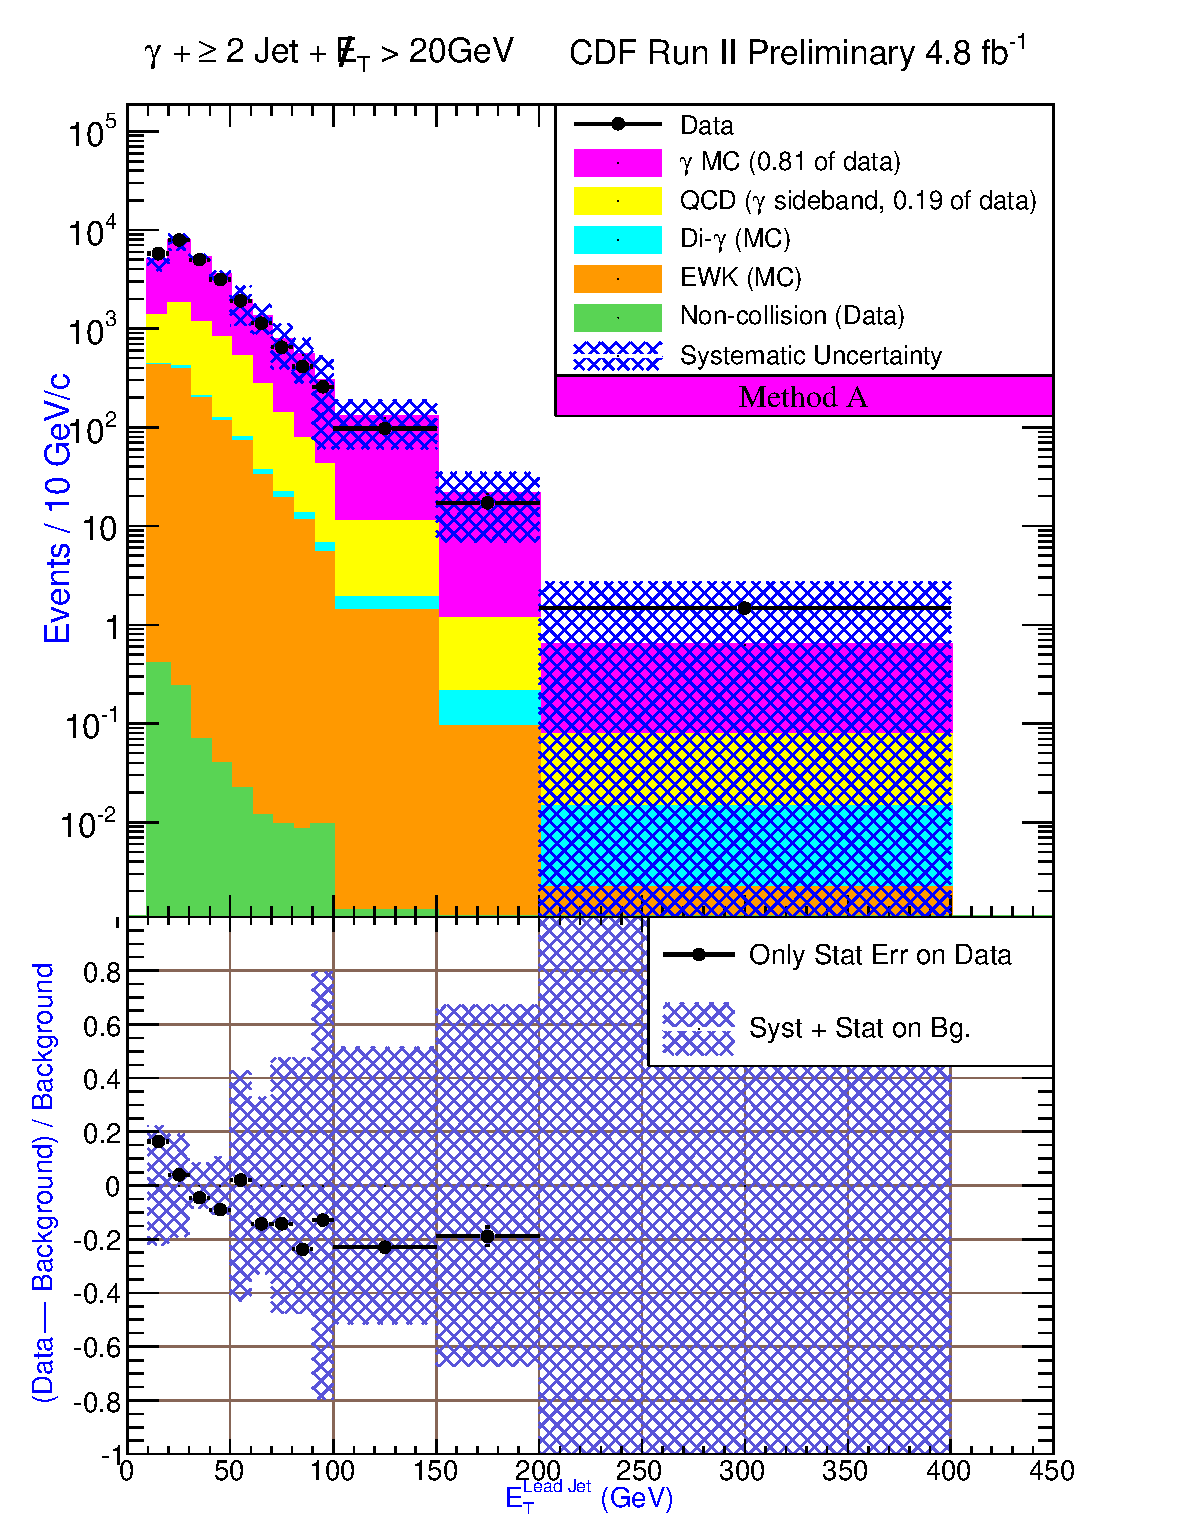
\includegraphics[scale=\resultsHistScale,keepaspectratio=true]{./g30jetmet20_MtdA_plot2_Et_j1.pdf}
 % g30jet_MtdA_plot1_Et_pho.pdf: 567x734 pixel, 72dpi, 20.00x25.89 cm, bb=0 0 567 734
}
 \caption{\newterm{Method A}: \et distribution of the leading jet in \phoonejetmettwenty (left) and \photwojetmettwenty (right) data samples.}
 \label{fig:Result_MtdA_gj1Met20_JetEt}
\end{figure}

\begin{figure}[h!]
 \centering
 \subfigure[]{
 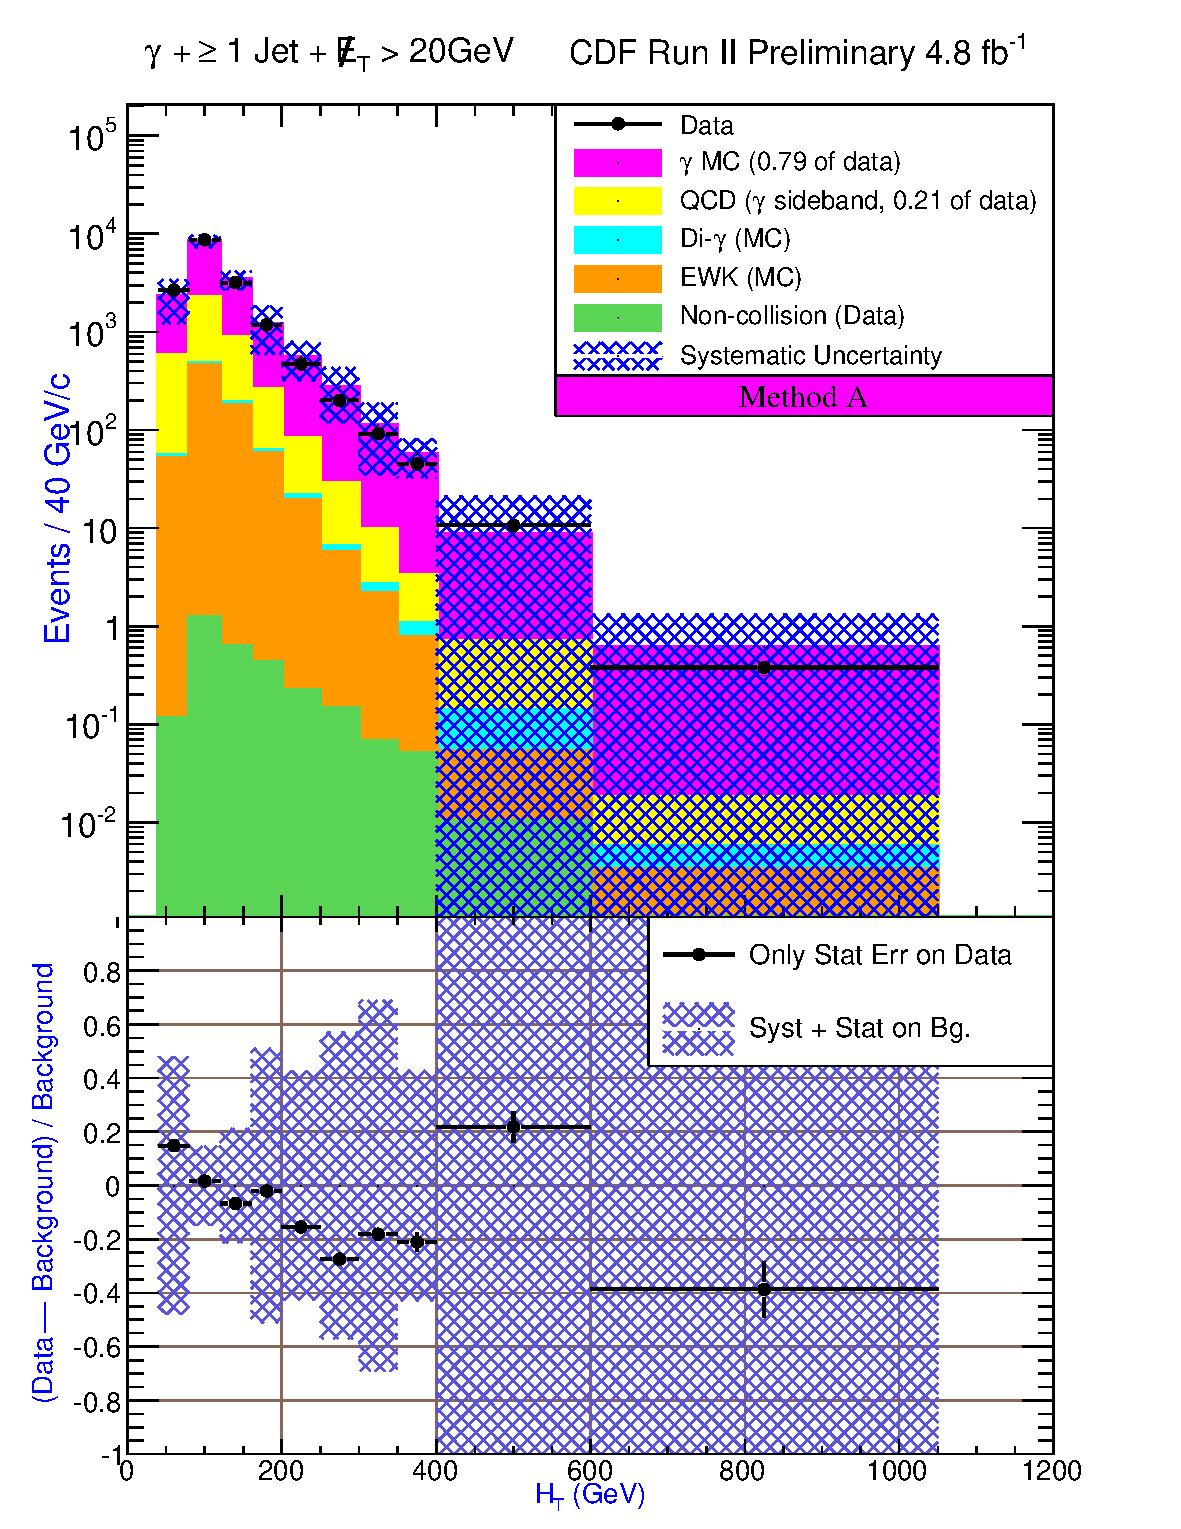
\includegraphics[scale=\resultsHistScale,keepaspectratio=true]{./g30jetmet20_MtdA_plot1_Ht.pdf}
 % g30jet_MtdA_plot1_Et_pho.pdf: 567x734 pixel, 72dpi, 20.00x25.89 cm, bb=0 0 567 734
}
 \subfigure[]{
 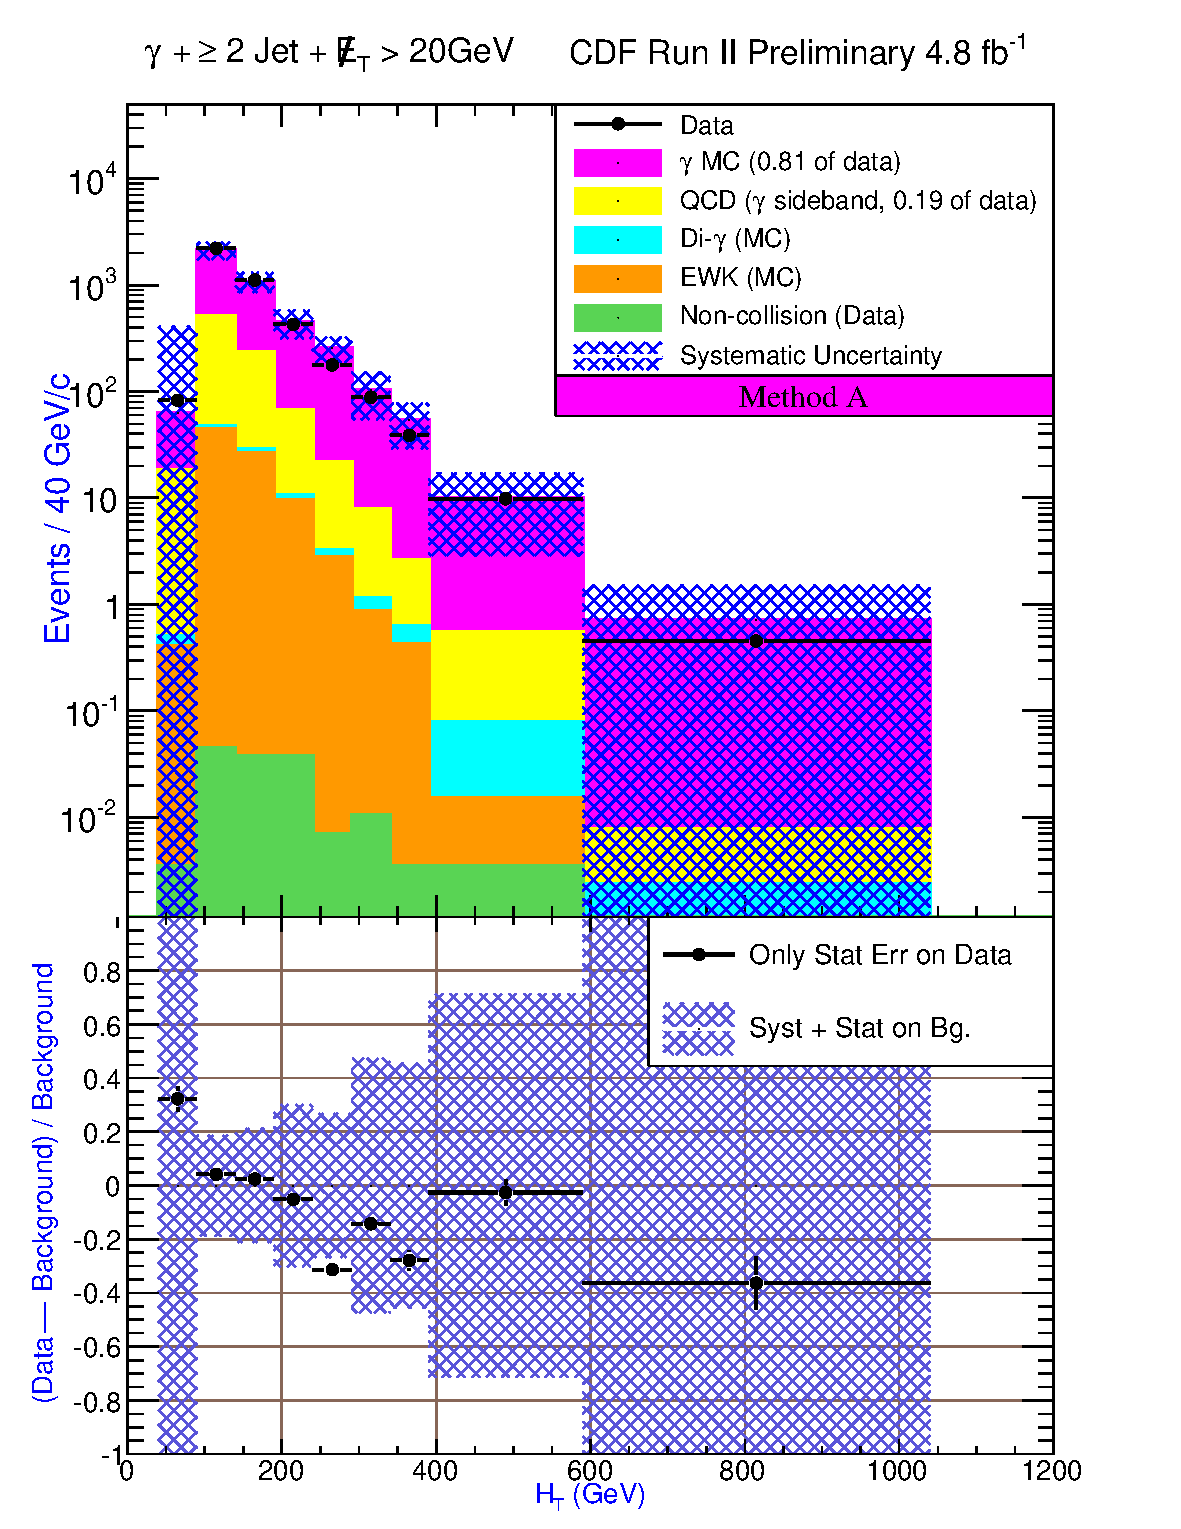
\includegraphics[scale=\resultsHistScale,keepaspectratio=true]{./g30jetmet20_MtdA_plot2_Ht.pdf}
 % g30jet_MtdA_plot1_Et_pho.pdf: 567x734 pixel, 72dpi, 20.00x25.89 cm, bb=0 0 567 734
}
 \caption{\newterm{Method A}: \Ht distribution of the leading jet in \phoonejetmettwenty (left) and \photwojetmettwenty (right) data samples.}
 \label{fig:Result_MtdA_gj1Met20_Ht}
\end{figure}

\begin{figure}[h!]
 \centering
\subfigure[]{
 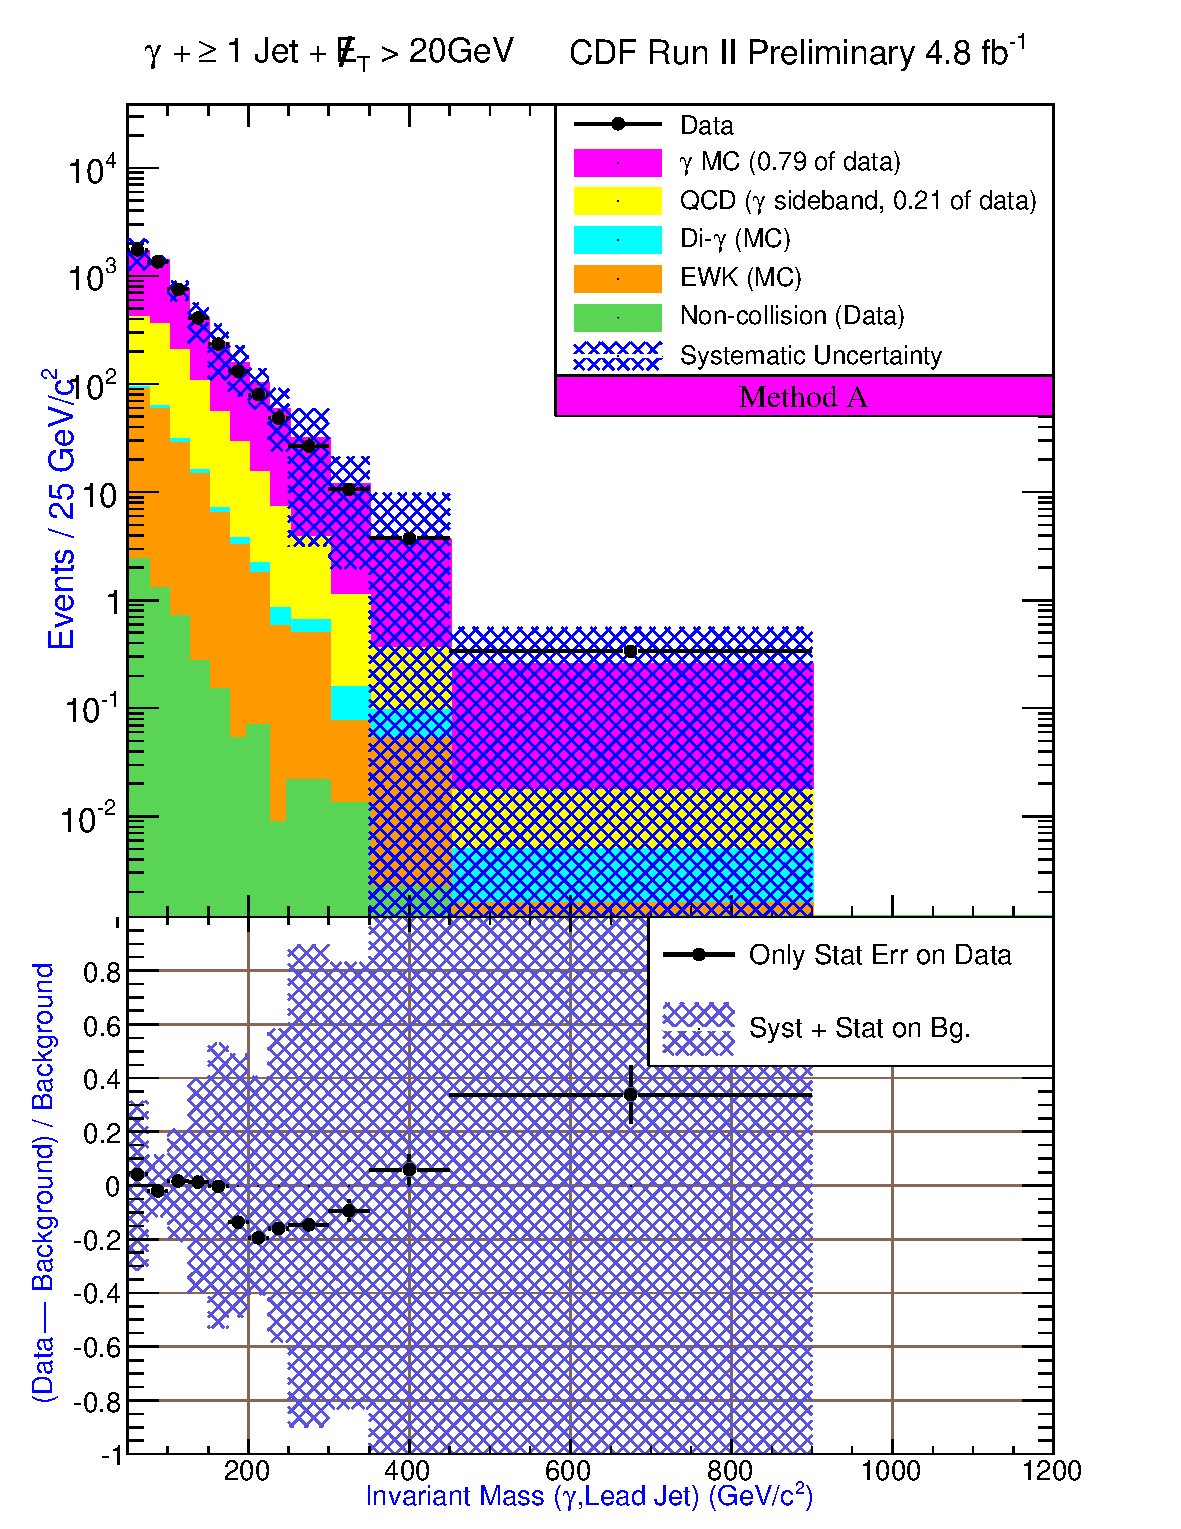
\includegraphics[scale=\resultsHistScale,keepaspectratio=true]{./g30jetmet20_MtdA_plot1_InvMass_pj1.pdf}
 % g30jet_MtdA_plot1_Et_pho.pdf: 567x734 pixel, 72dpi, 20.00x25.89 cm, bb=0 0 567 734
}
\subfigure[]{
 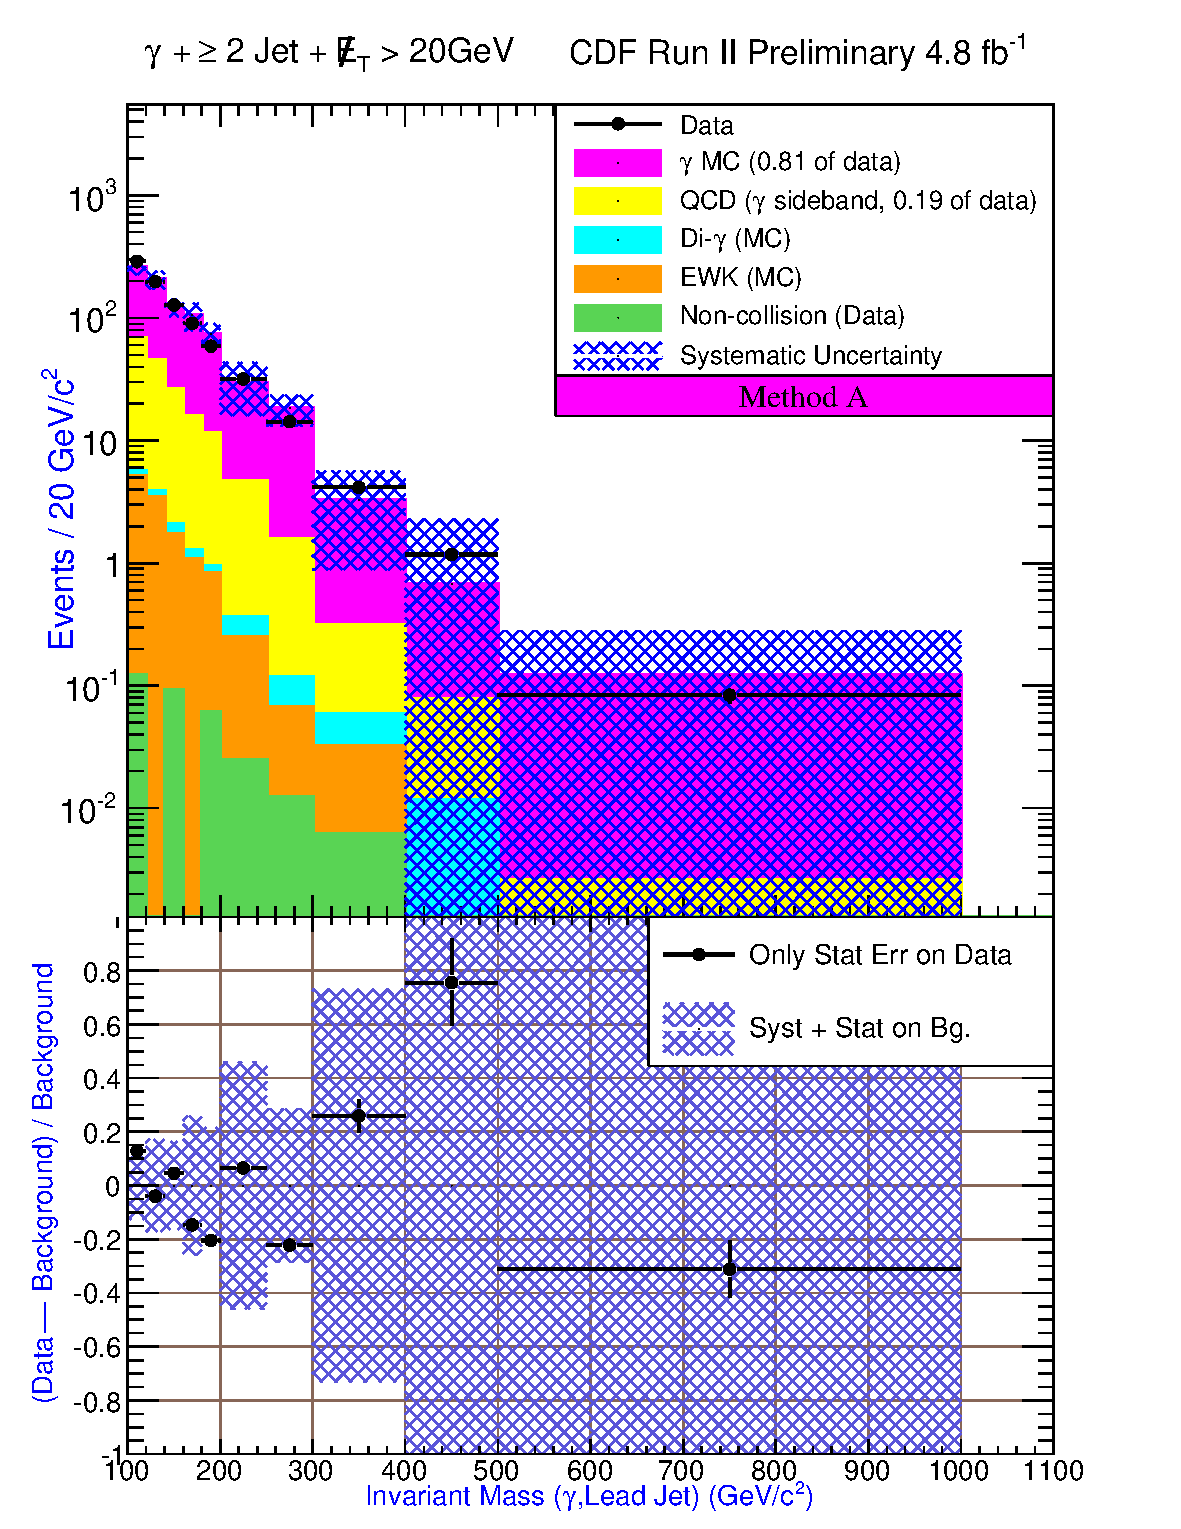
\includegraphics[scale=\resultsHistScale,keepaspectratio=true]{./g30jetmet20_MtdA_plot2_InvMass_pj1.pdf}
 % g30jet_MtdA_plot1_Et_pho.pdf: 567x734 pixel, 72dpi, 20.00x25.89 cm, bb=0 0 567 734
}
 \caption{\newterm{Method A}: Invariant mass of the photon and the leading jet distributions of the leading jet in \phoonejetmettwenty (left) and \photwojetmettwenty (right) data samples.}
 \label{fig:Result_MtdA_gj1Met20_Mass_gj1}
\end{figure}

\begin{figure}[h!]
 \centering
\subfigure[]{
 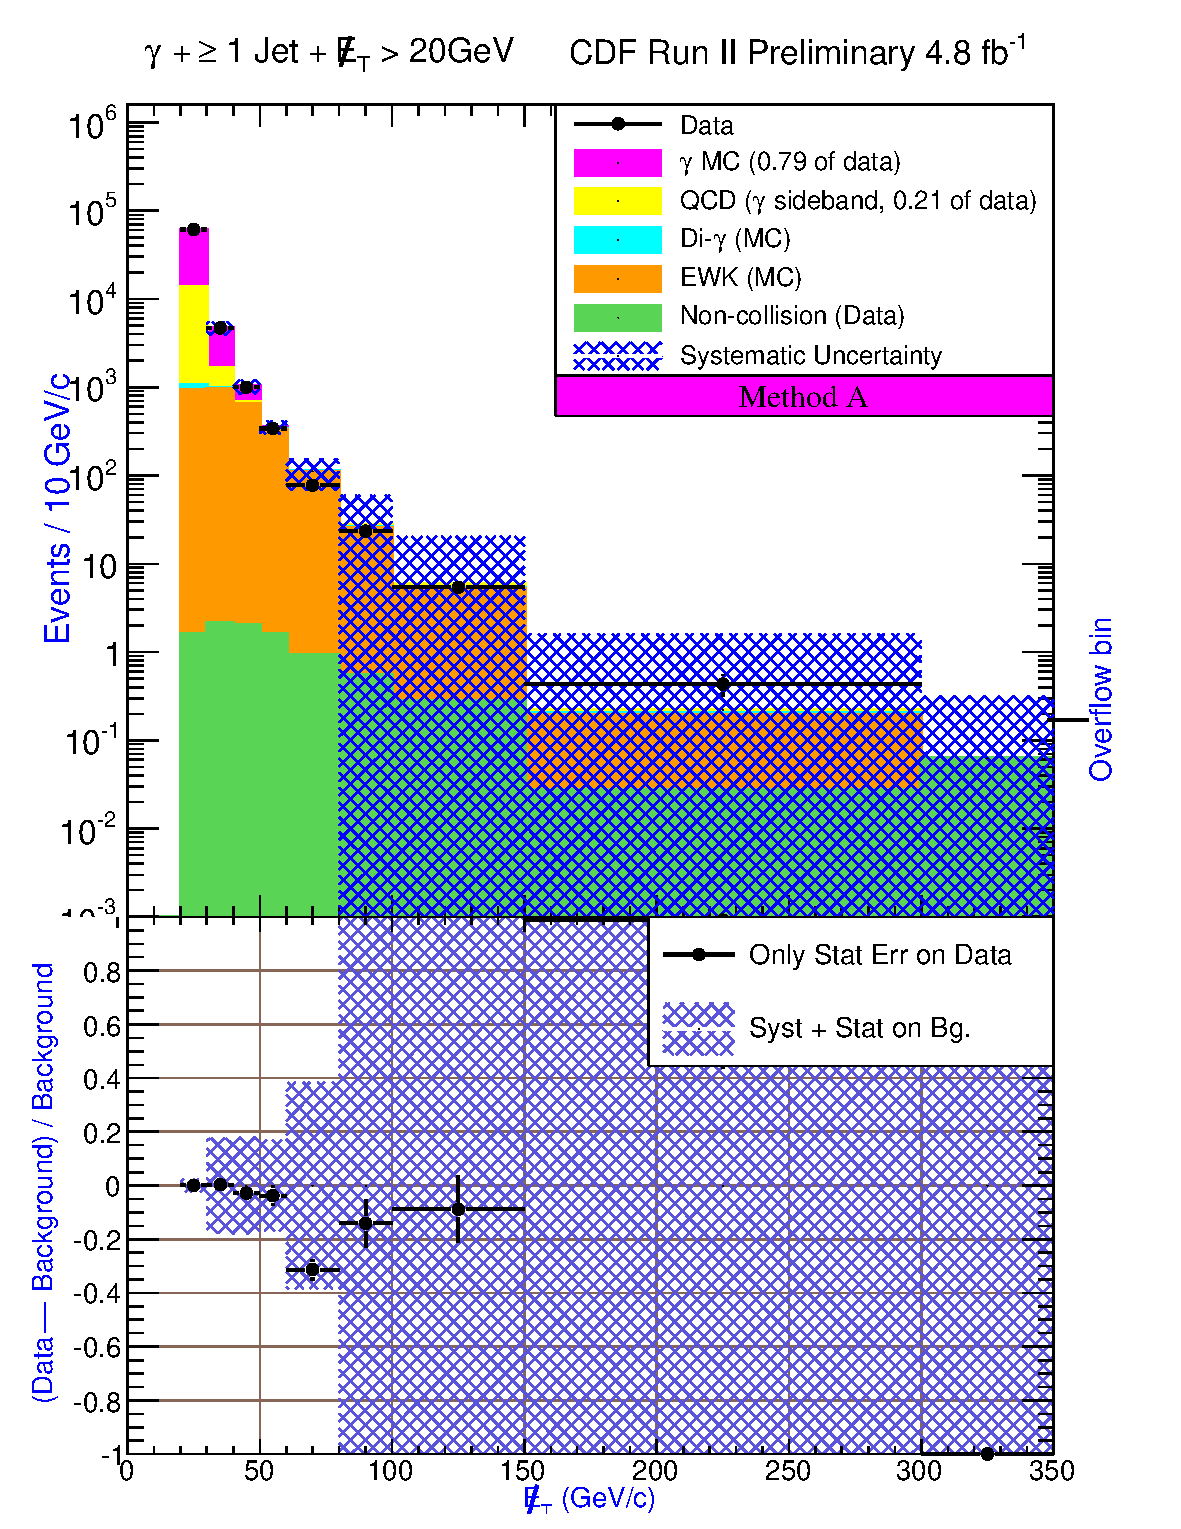
\includegraphics[scale=\resultsHistScale,keepaspectratio=true]{./g30jetmet20_MtdA_plot1_Met.pdf}
 % g30jet_MtdA_plot1_Et_pho.pdf: 567x734 pixel, 72dpi, 20.00x25.89 cm, bb=0 0 567 734
}
\subfigure[]{
 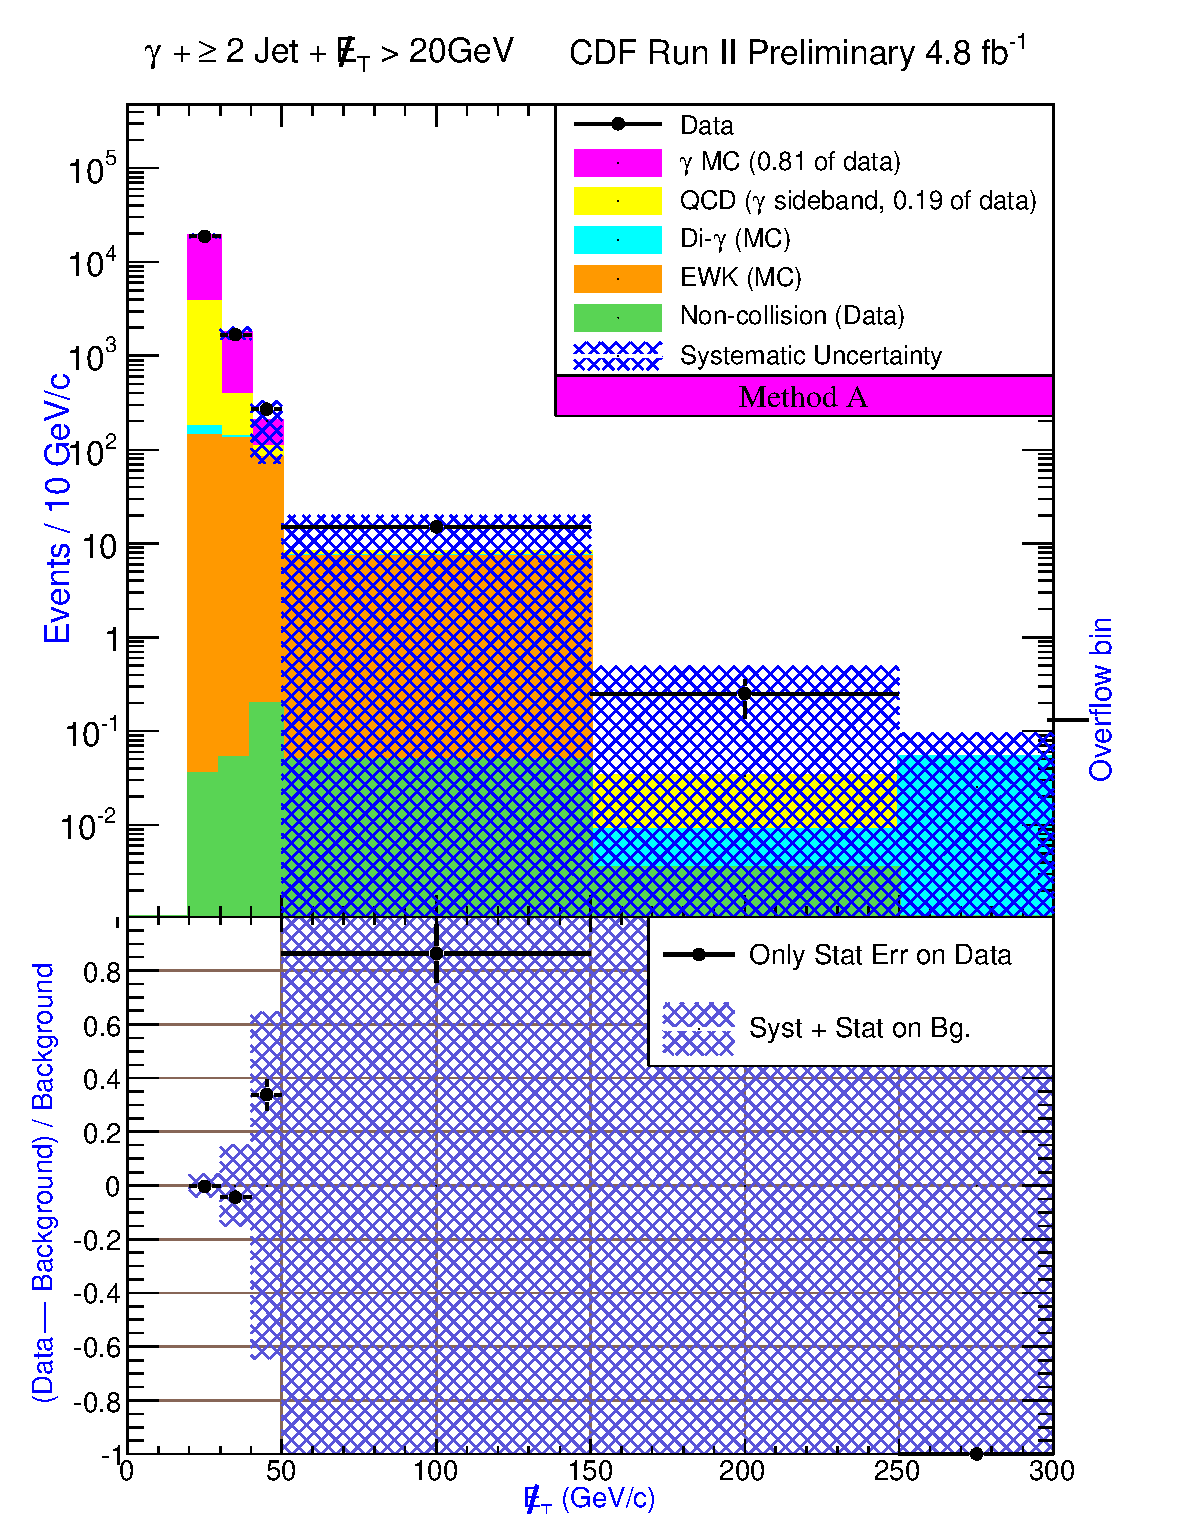
\includegraphics[scale=\resultsHistScale,keepaspectratio=true]{./g30jetmet20_MtdA_plot2_Met.pdf}
 % g30jet_MtdA_plot1_Et_pho.pdf: 567x734 pixel, 72dpi, 20.00x25.89 cm, bb=0 0 567 734
}
 \caption{\newterm{Method A}: \met distribution of the leading jet in \phoonejetmettwenty (left) and \photwojetmettwenty (right) data samples.}
 \label{fig:Result_MtdA_gj1Met20_Met}
\end{figure}

\begin{figure}[h!]
 \centering
\subfigure[]{
 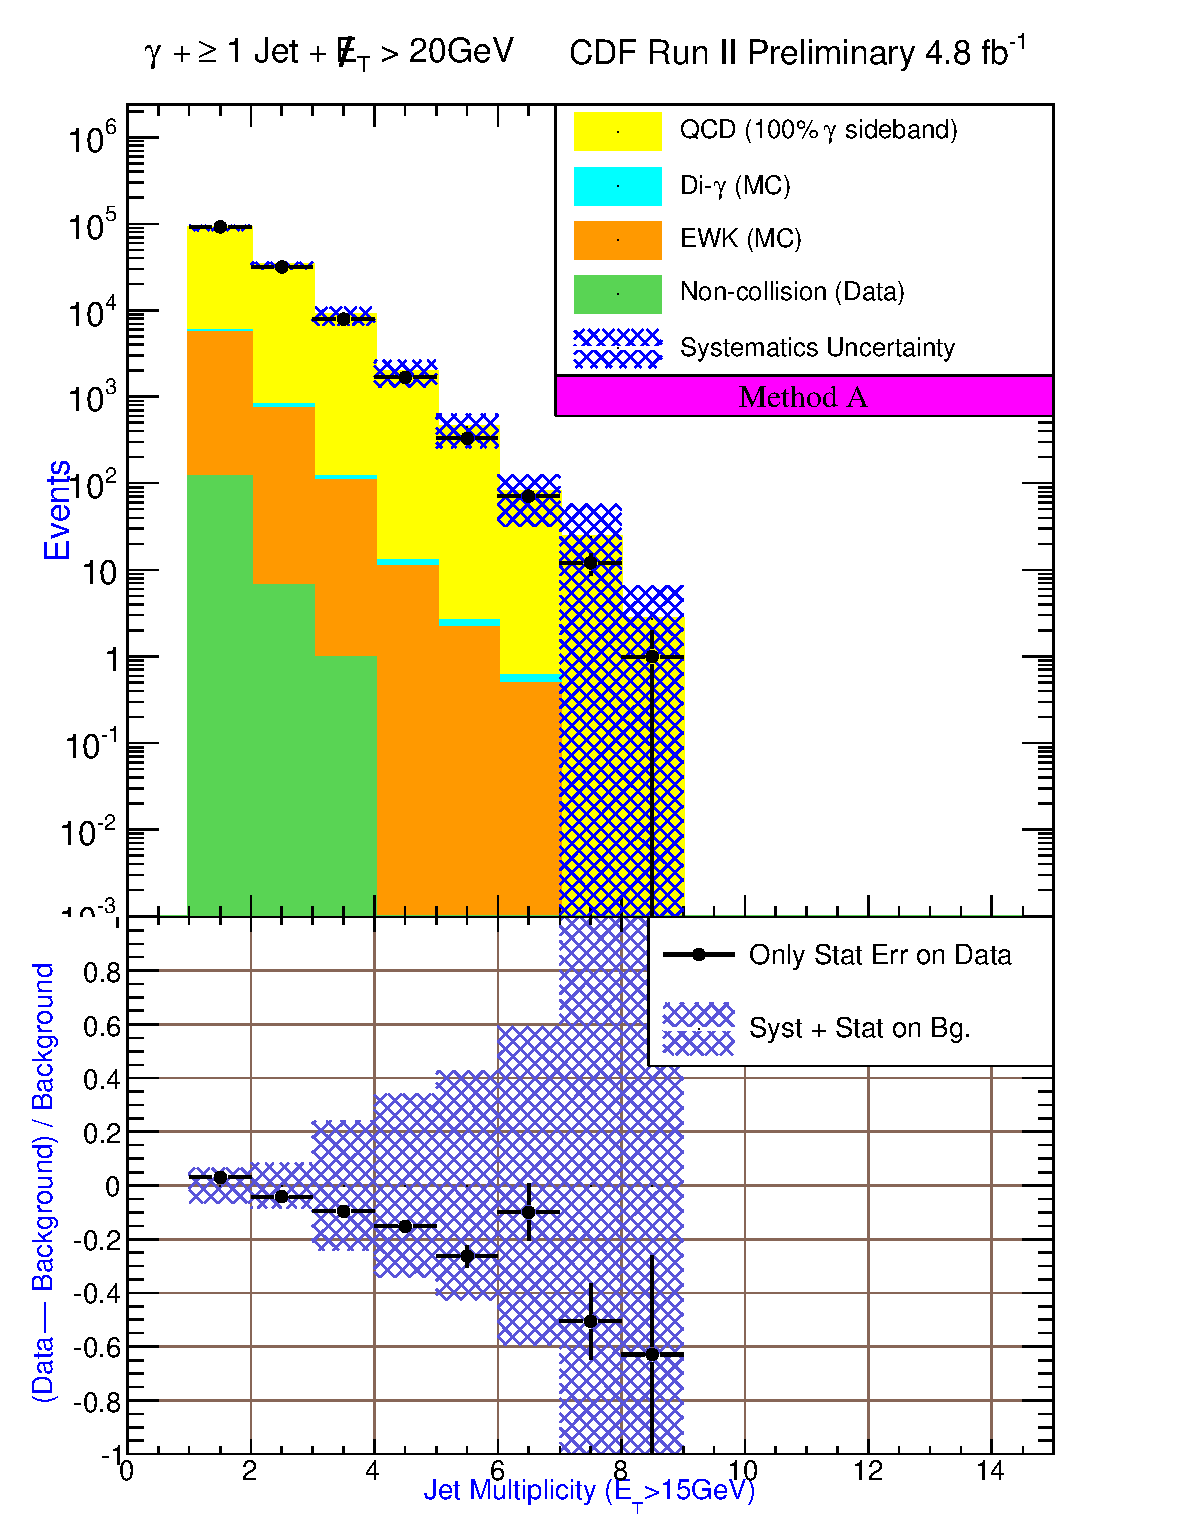
\includegraphics[scale=\resultsHistScale,keepaspectratio=true]{./g30jetmet20_MtdA_plot1_NJet.pdf}
  %g30jet_MtdA_plot1_Et_pho.pdf: 567x734 pixel, 72dpi, 20.00x25.89 cm, bb=0 0 567 734
}
\caption{\newterm{Method A}: Jet Multiplicity distribution of the leading jet in \phoonejetmettwenty data sample.}
 \label{fig:Result_MtdA_gj1Met20_Njet}
\end{figure}


\begin{figure}[h!]
 \centering
\subfigure[]{
 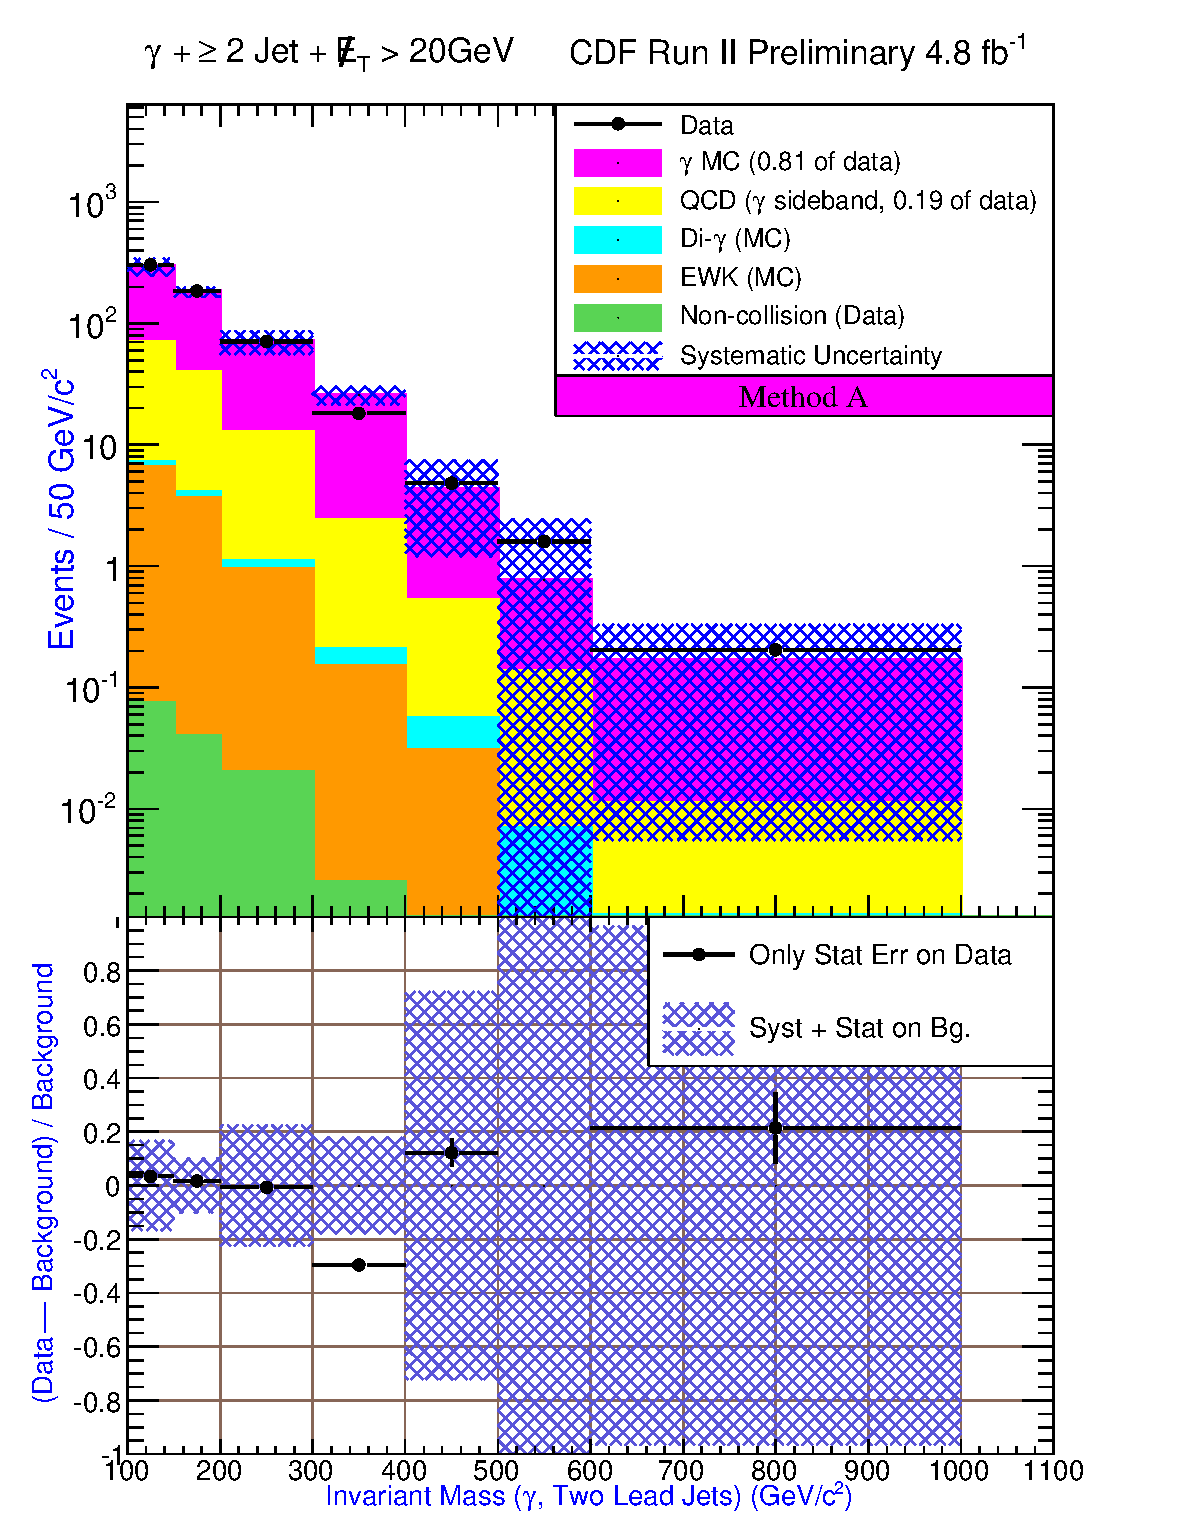
\includegraphics[scale=\resultsHistScale,keepaspectratio=true]{./g30jetmet20_MtdA_plot2_InvMass_pj1j2.pdf}
 % g30jet_MtdA_plot1_Et_pho.pdf: 567x734 pixel, 72dpi, 20.00x25.89 cm, bb=0 0 567 734
}
\subfigure[]{
 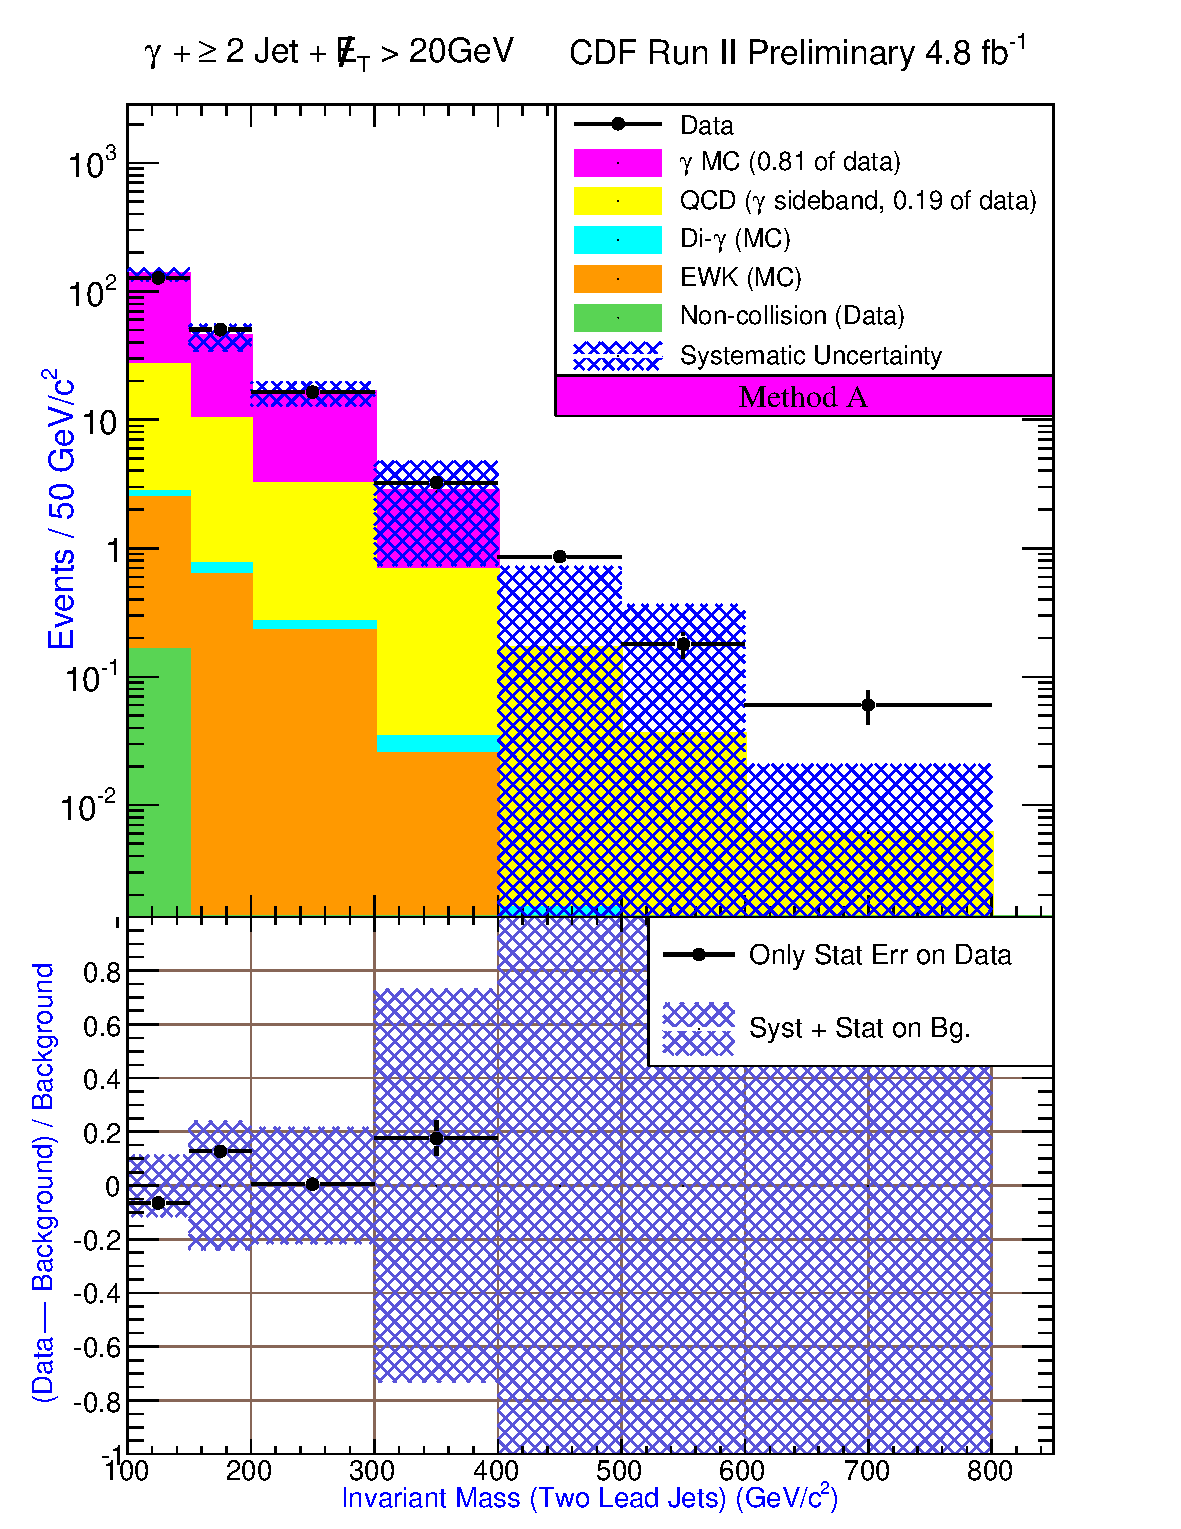
\includegraphics[scale=\resultsHistScale,keepaspectratio=true]{./g30jetmet20_MtdA_plot2_InvMass_j1j2.pdf}
 % g30jet_MtdA_plot1_Et_pho.pdf: 567x734 pixel, 72dpi, 20.00x25.89 cm, bb=0 0 567 734
}
 \caption{\newterm{Method A}: Invariant mass of the photon and the two leading jets (left) and the invariant mass of the two leading jets (right), in \photwojetmettwenty data sample.}
 \label{fig:Result_MtdA_gj2Met20_Mass_gj1j2}
\end{figure}


%%%%%%%%%%%%%%%%%%%%%%%%%%%%%%%%%%
%%% METHOD B PLOTS:
%%%%%%%%%%%%%%%%%%%%%%%%%%%%%%%%%%
\begin{figure}[h!]
 \centering
\subfigure[]{
 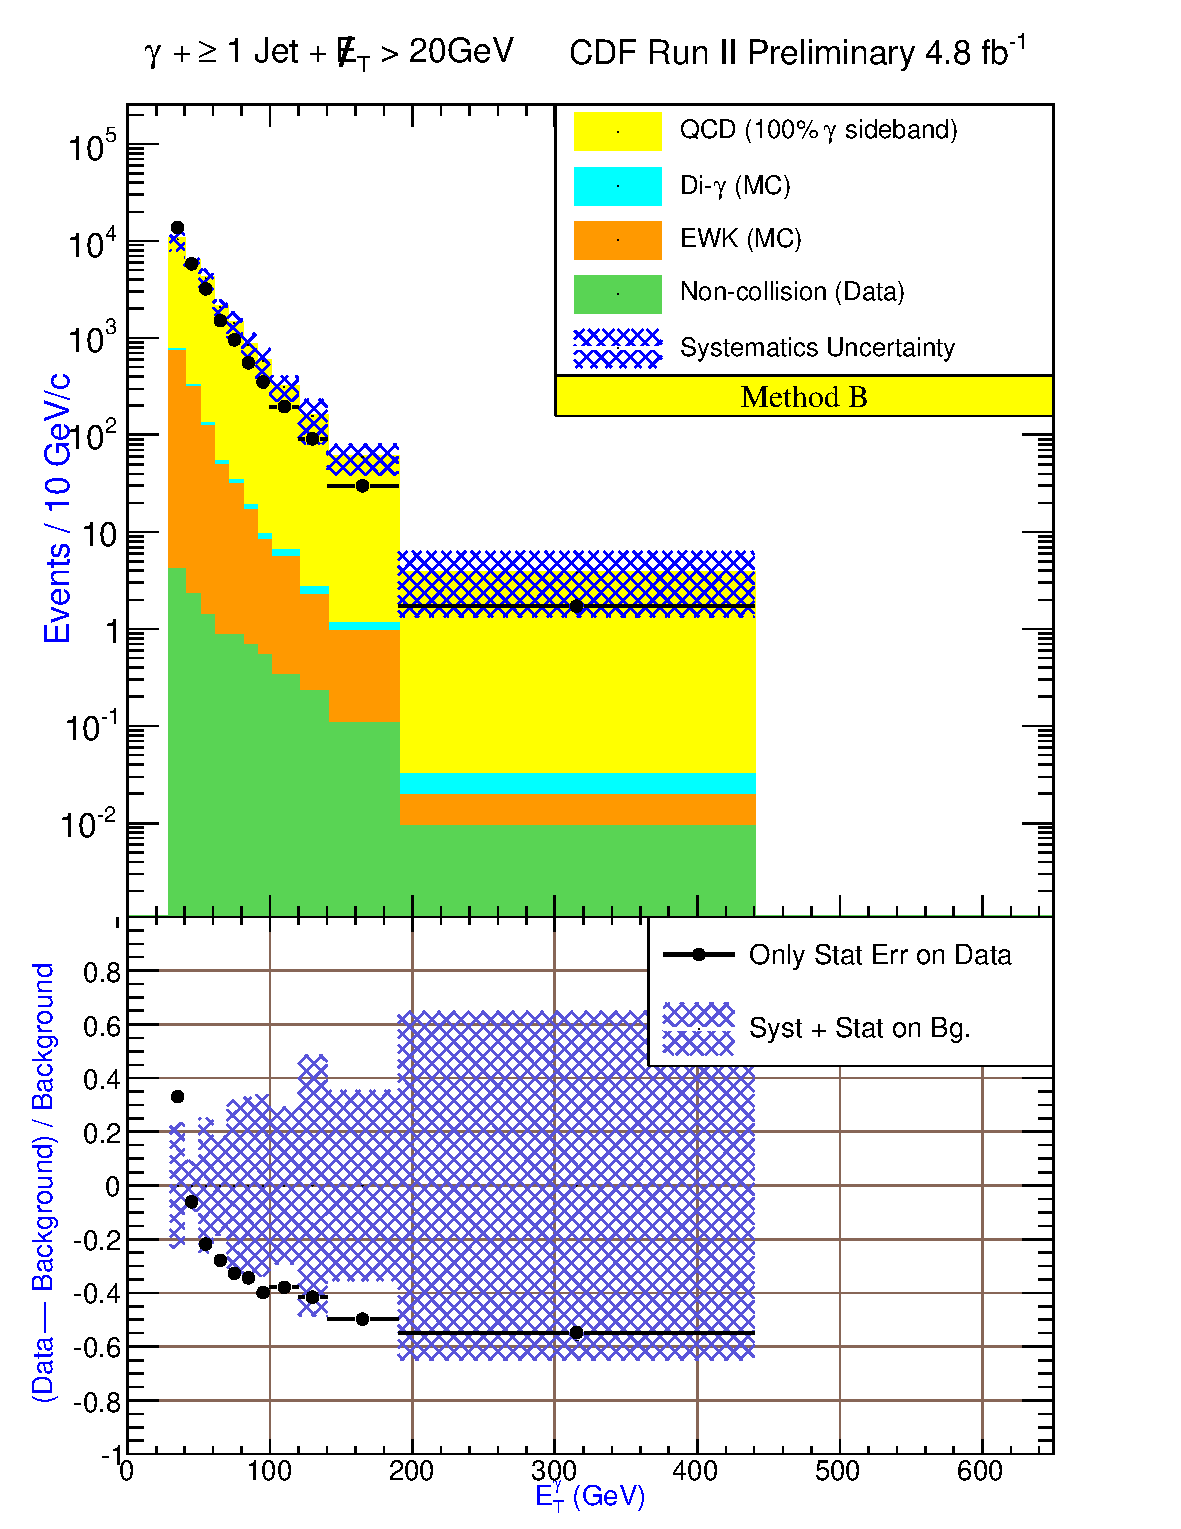
\includegraphics[scale=\resultsHistScale,keepaspectratio=true]{./g30jetmet20_MtdB_plot1_Et_pho.pdf}
 % g30jet_MtdB_plot1_Et_pho.pdf: 567x734 pixel, 72dpi, 20.00x25.89 cm, bb=0 0 567 734
}
\subfigure[]{
 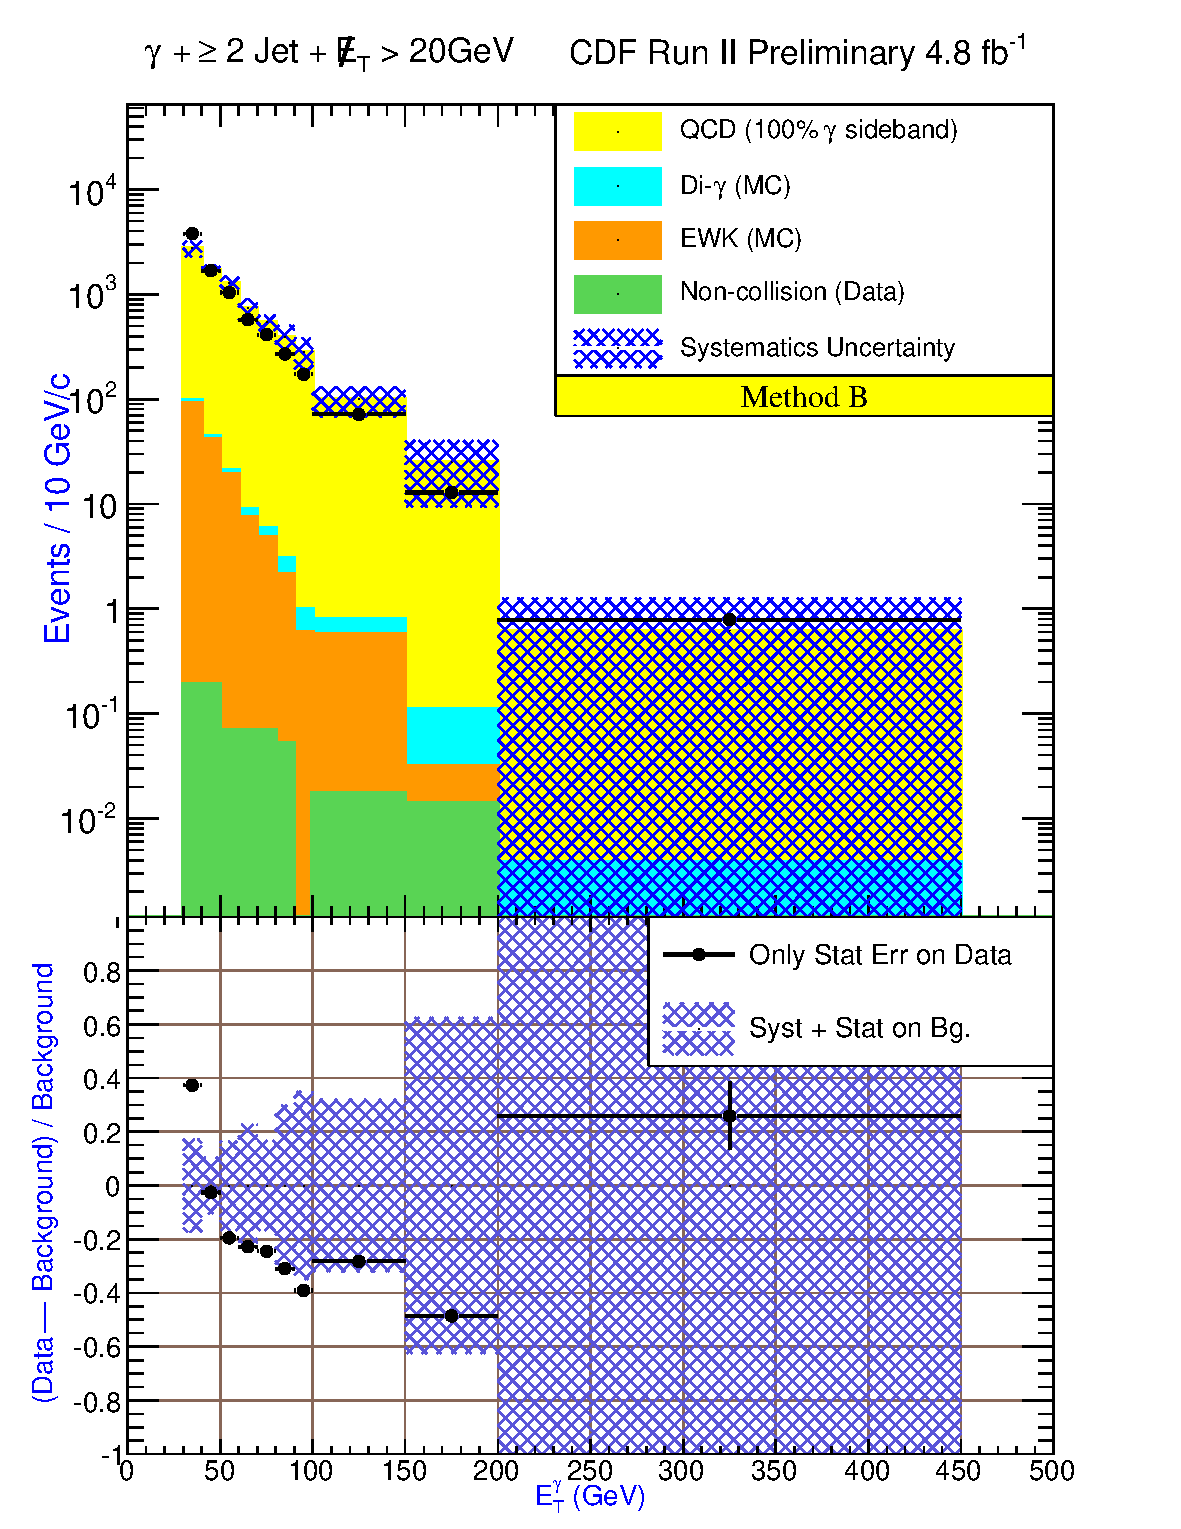
\includegraphics[scale=\resultsHistScale,keepaspectratio=true]{./g30jetmet20_MtdB_plot2_Et_pho.pdf}
 % g30jet_MtdB_plot1_Et_pho.pdf: 567x734 pixel, 72dpi, 20.00x25.89 cm, bb=0 0 567 734
}

 \caption{\newterm{Method B}: Photon \et distribution of the \phoonejetmettwenty (left) and \photwojetmettwenty (right) data samples.}
 \label{fig:Result_MtdB_gj1Met20_PhoEt}
\end{figure}

\begin{figure}[h!]
 \centering
\subfigure[]{
 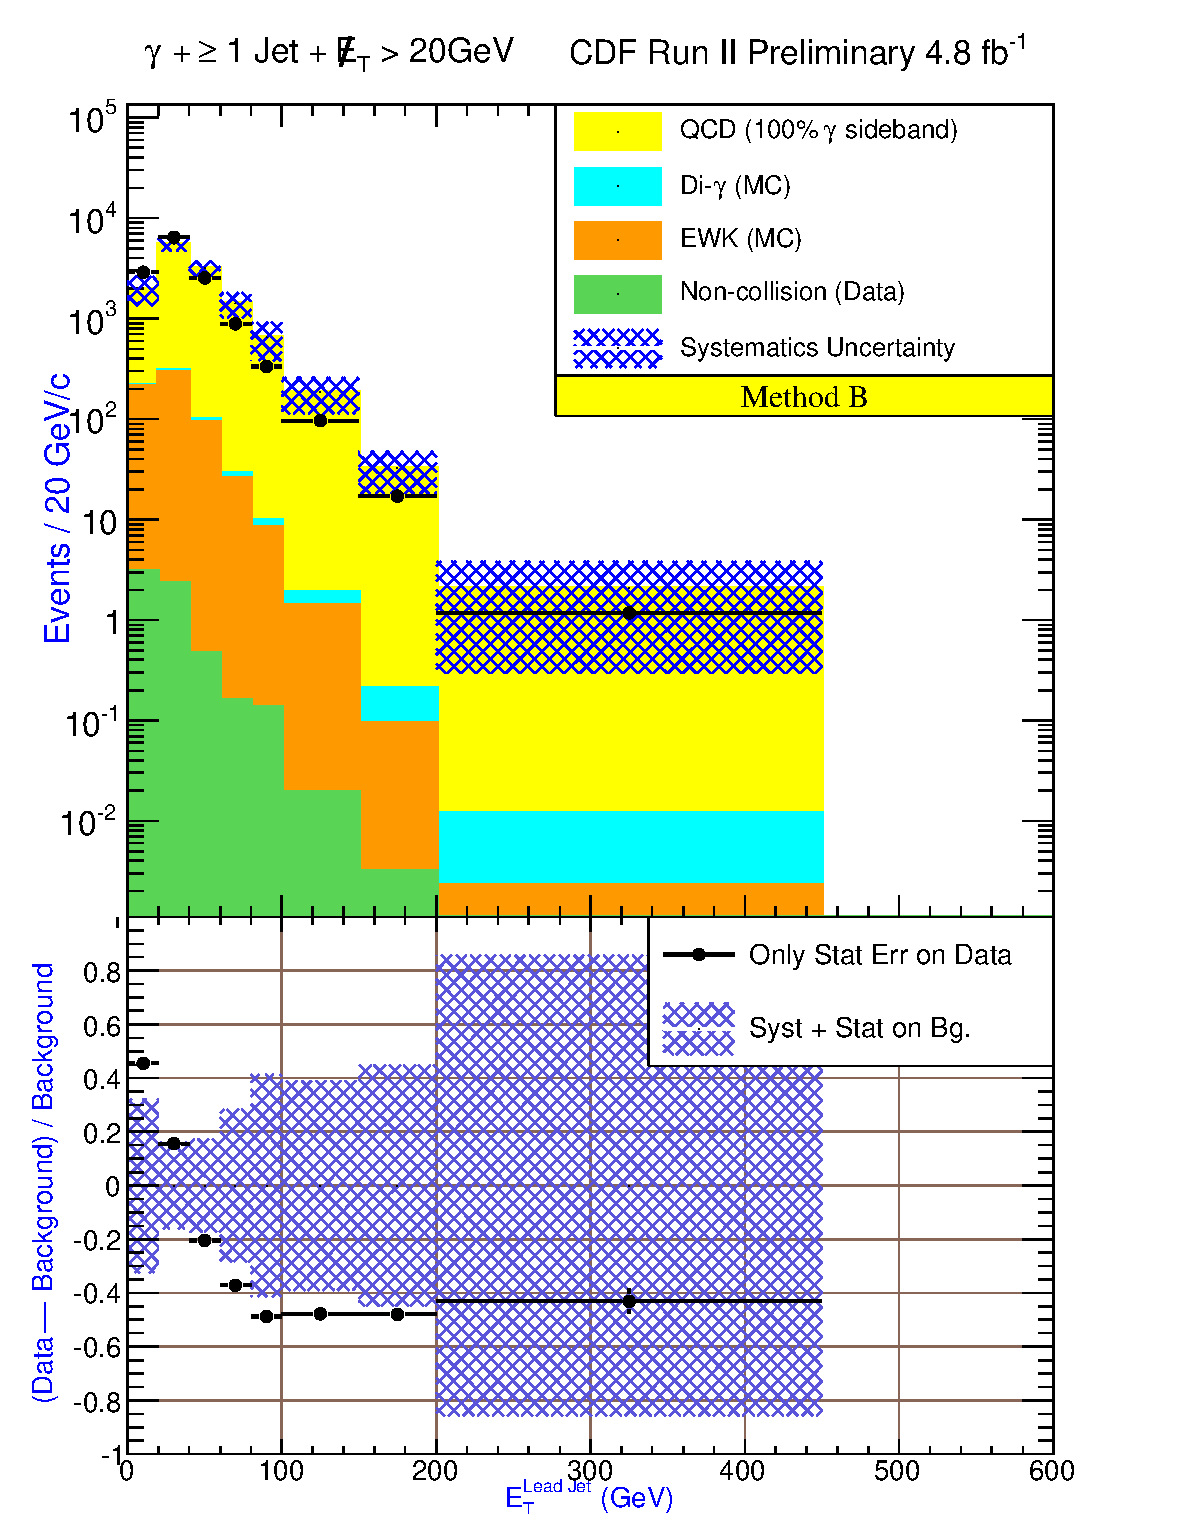
\includegraphics[scale=\resultsHistScale,keepaspectratio=true]{./g30jetmet20_MtdB_plot1_Et_j1.pdf}
 % g30jet_MtdB_plot1_Et_pho.pdf: 567x734 pixel, 72dpi, 20.00x25.89 cm, bb=0 0 567 734
}
\subfigure[]{
 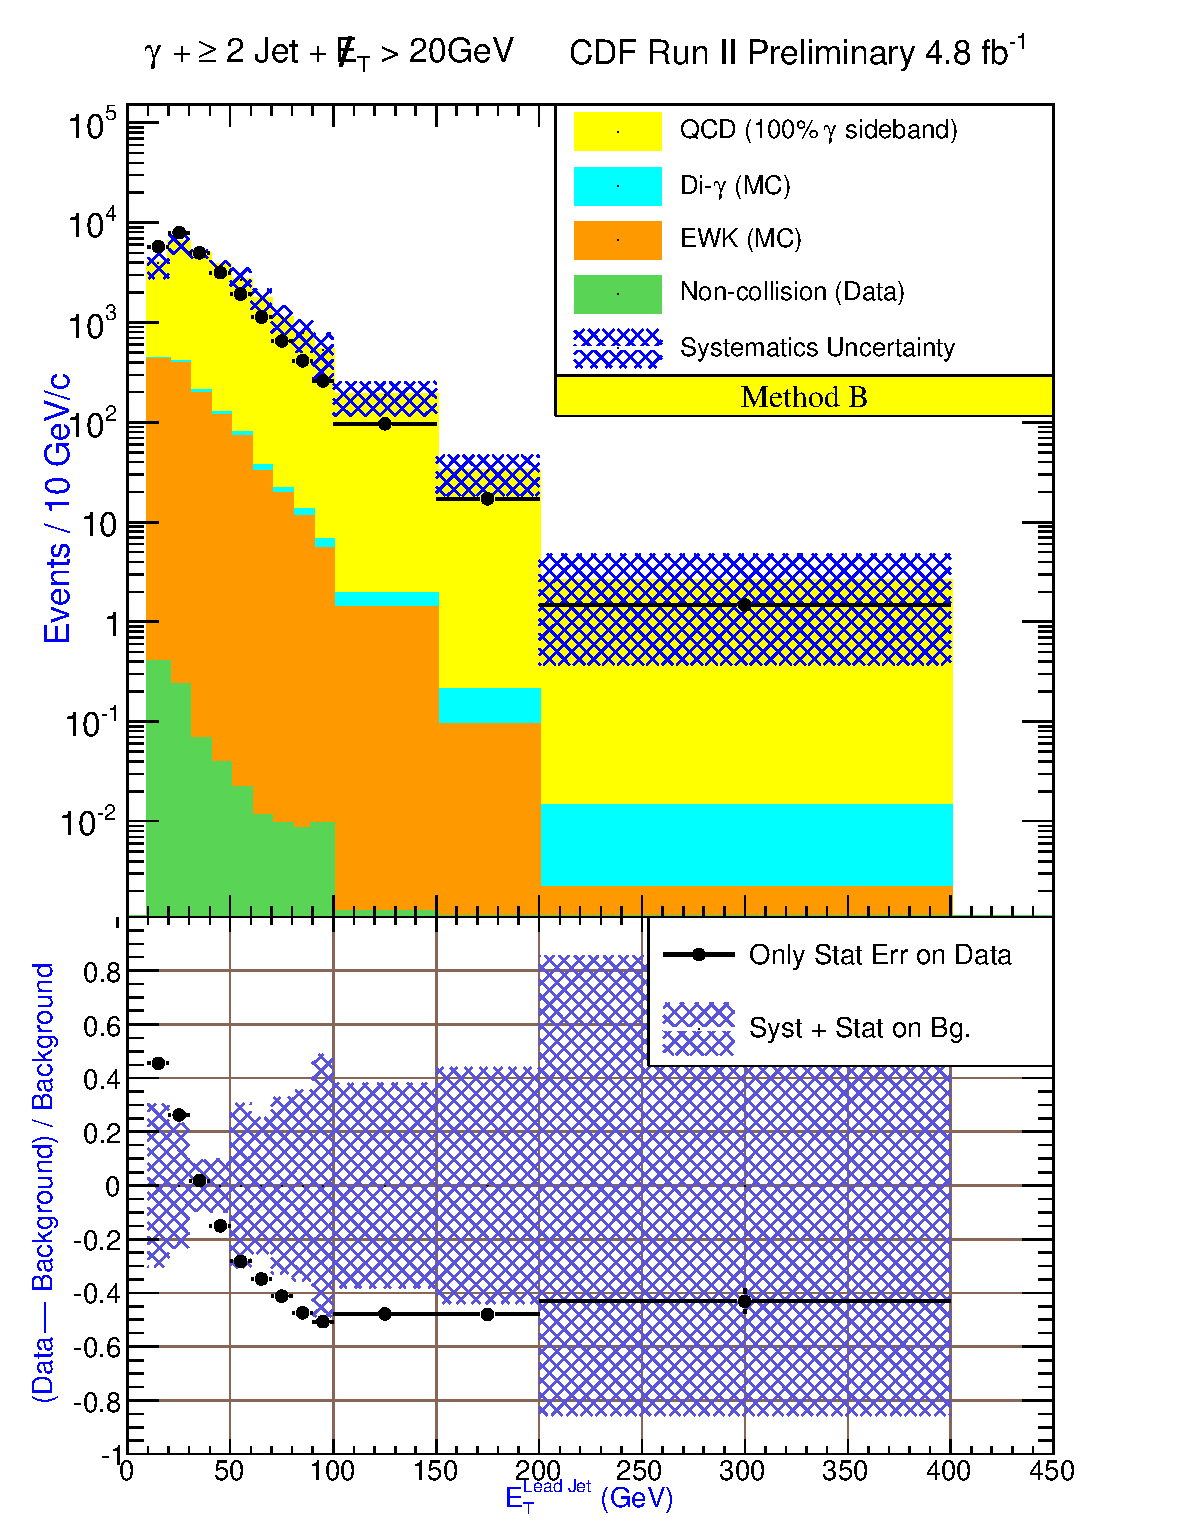
\includegraphics[scale=\resultsHistScale,keepaspectratio=true]{./g30jetmet20_MtdB_plot2_Et_j1.pdf}
 % g30jet_MtdB_plot1_Et_pho.pdf: 567x734 pixel, 72dpi, 20.00x25.89 cm, bb=0 0 567 734
}
 \caption{\newterm{Method B}: \et distribution of the leading jet in \phoonejetmettwenty (left) and \photwojetmettwenty (right) data samples.}
 \label{fig:Result_MtdB_gj1Met20_JetEt}
\end{figure}

\begin{figure}[h!]
 \centering
 \subfigure[]{
 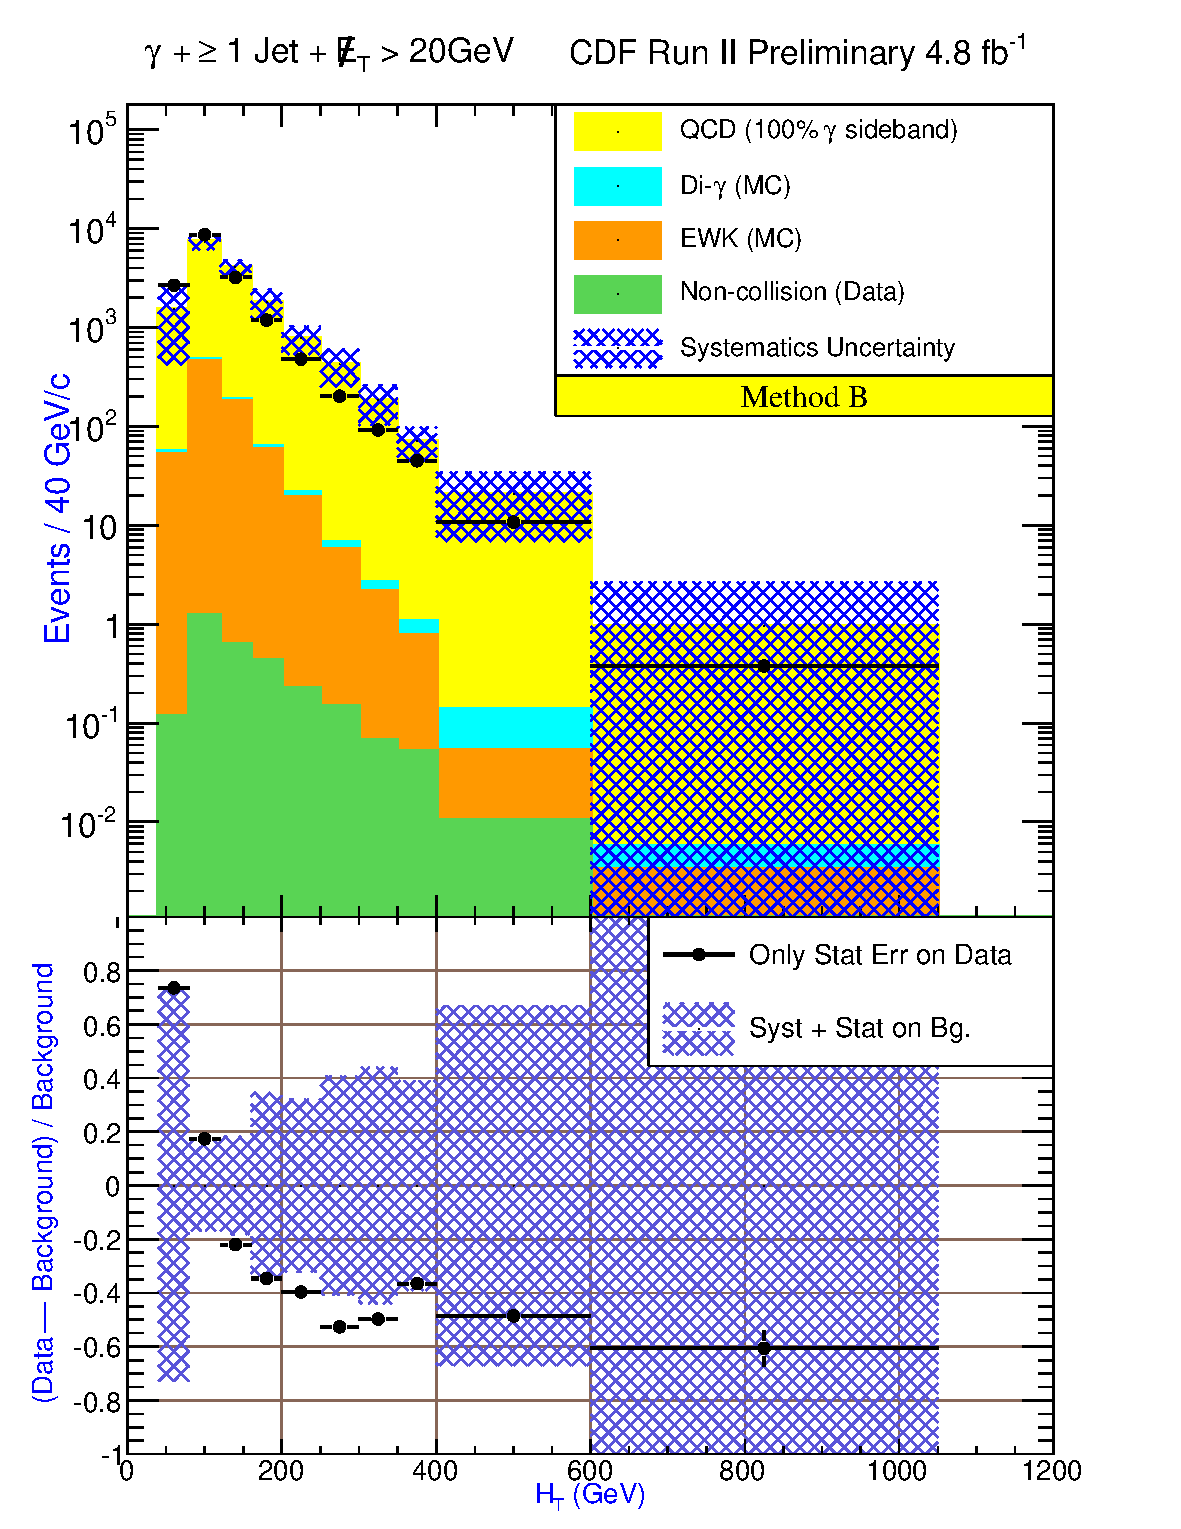
\includegraphics[scale=\resultsHistScale,keepaspectratio=true]{./g30jetmet20_MtdB_plot1_Ht.pdf}
 % g30jet_MtdB_plot1_Et_pho.pdf: 567x734 pixel, 72dpi, 20.00x25.89 cm, bb=0 0 567 734
}
 \subfigure[]{
 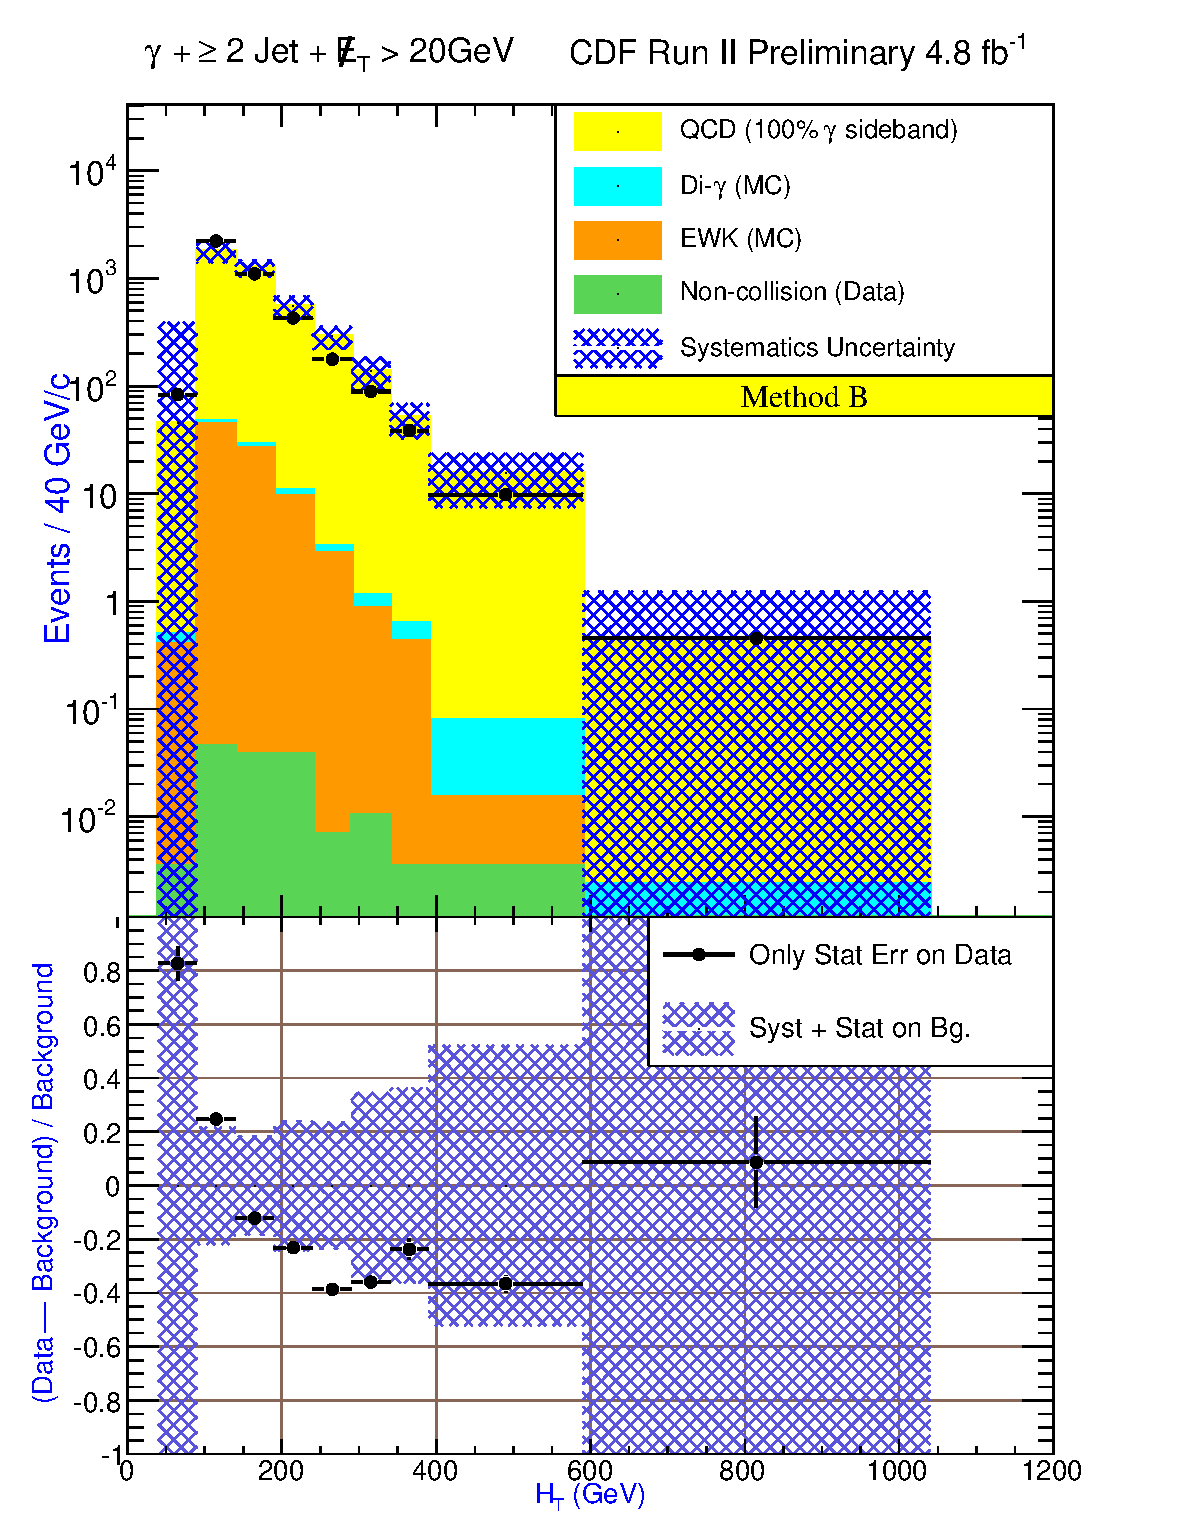
\includegraphics[scale=\resultsHistScale,keepaspectratio=true]{./g30jetmet20_MtdB_plot2_Ht.pdf}
 % g30jet_MtdB_plot1_Et_pho.pdf: 567x734 pixel, 72dpi, 20.00x25.89 cm, bb=0 0 567 734
}
 \caption{\newterm{Method B}: \Ht distribution of the leading jet in \phoonejetmettwenty (left) and \photwojetmettwenty (right) data samples.}
 \label{fig:Result_MtdB_gj1Met20_Ht}
\end{figure}

\begin{figure}[h!]
 \centering
\subfigure[]{
 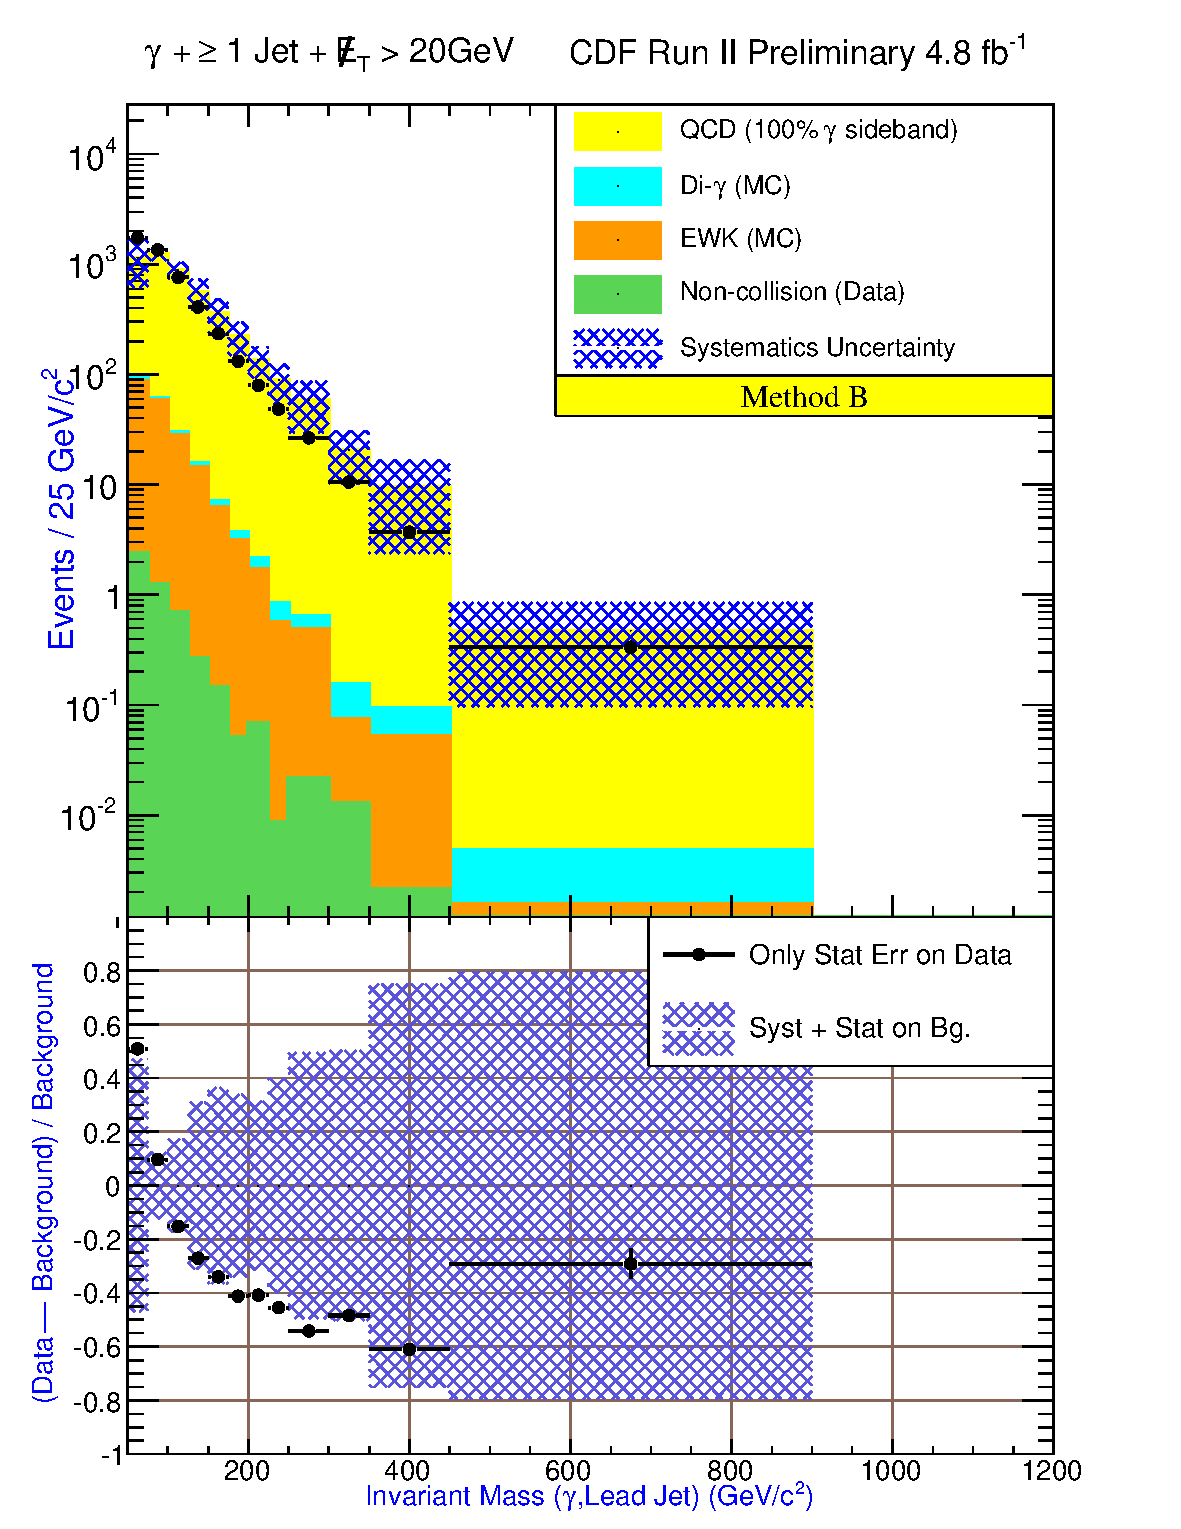
\includegraphics[scale=\resultsHistScale,keepaspectratio=true]{./g30jetmet20_MtdB_plot1_InvMass_pj1.pdf}
 % g30jet_MtdB_plot1_Et_pho.pdf: 567x734 pixel, 72dpi, 20.00x25.89 cm, bb=0 0 567 734
}
\subfigure[]{
 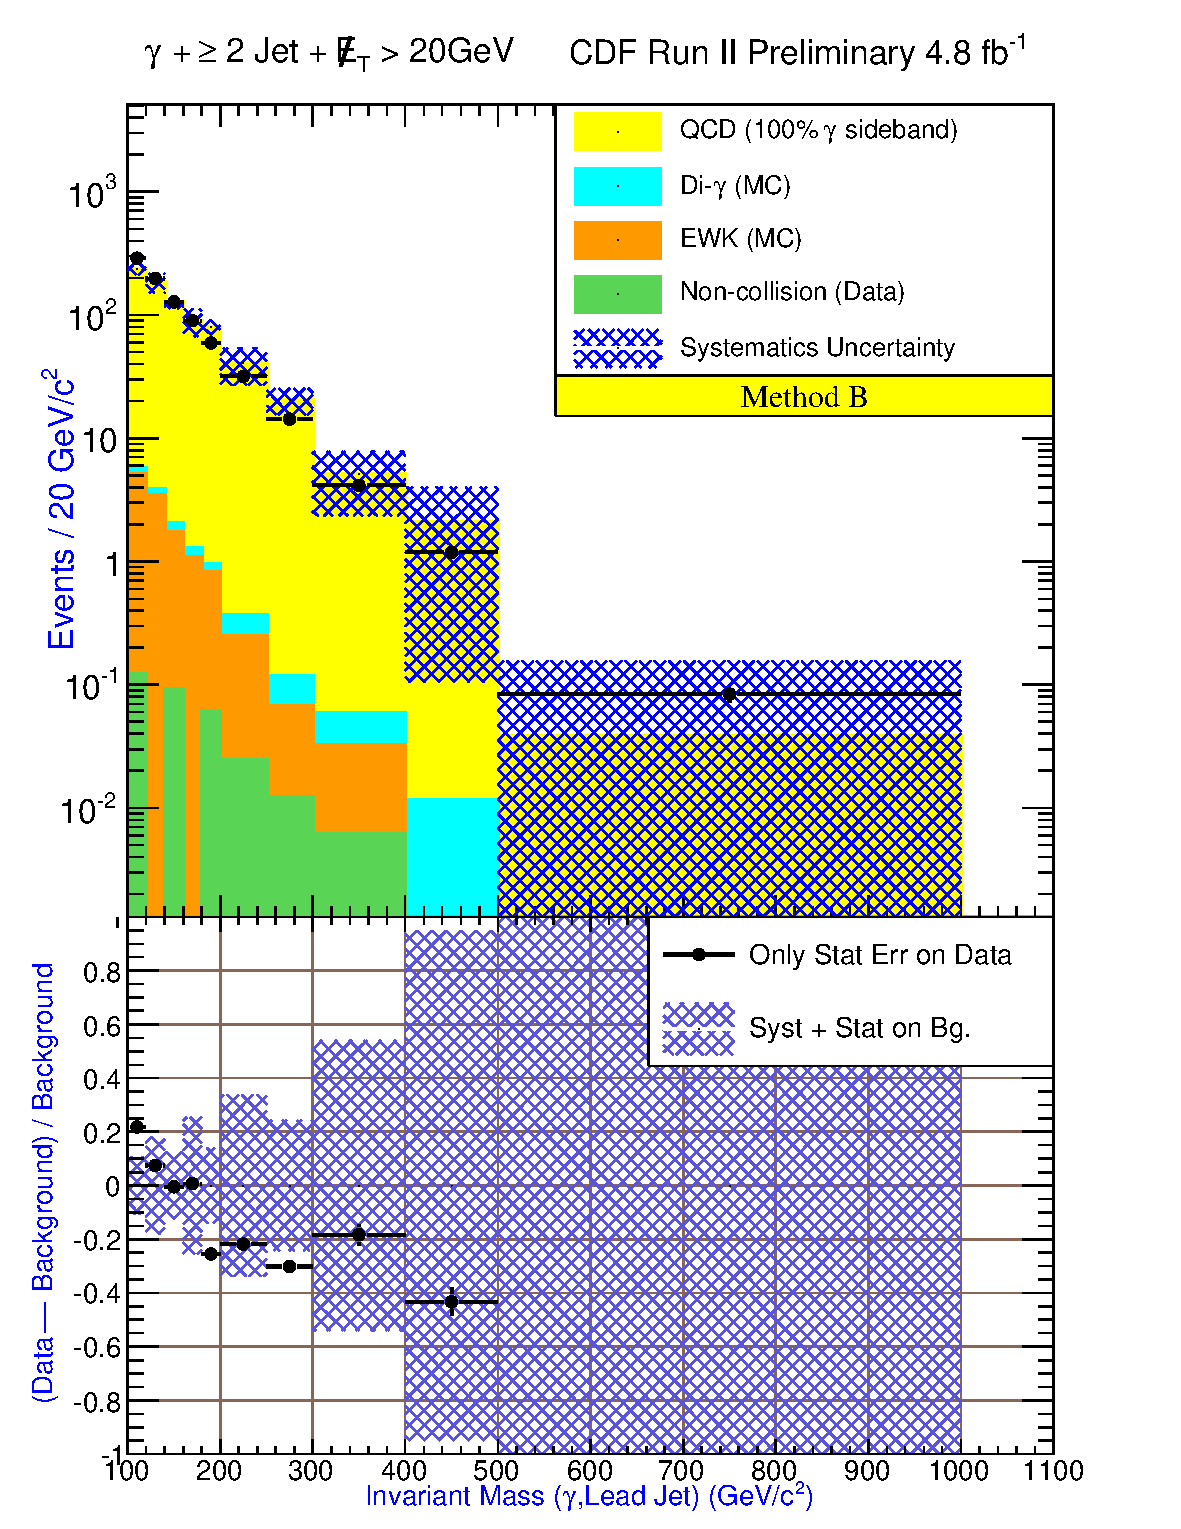
\includegraphics[scale=\resultsHistScale,keepaspectratio=true]{./g30jetmet20_MtdB_plot2_InvMass_pj1.pdf}
 % g30jet_MtdB_plot1_Et_pho.pdf: 567x734 pixel, 72dpi, 20.00x25.89 cm, bb=0 0 567 734
}
 \caption{\newterm{Method B}: Invariant mass of the photon and the leading jet distributions of the leading jet in \phoonejetmettwenty (left) and \photwojetmettwenty (right) data samples.}
 \label{fig:Result_MtdB_gj1Met20_Mass_gj1}
\end{figure}

\begin{figure}[h!]
 \centering
\subfigure[]{
 \includegraphics[scale=\resultsHistScale,keepaspectratio=true]{./g30jetmet20_MtdB_plot1_Met.pdf}
 % g30jet_MtdB_plot1_Et_pho.pdf: 567x734 pixel, 72dpi, 20.00x25.89 cm, bb=0 0 567 734
}
\subfigure[]{
 \includegraphics[scale=\resultsHistScale,keepaspectratio=true]{./g30jetmet20_MtdB_plot2_Met.pdf}
 % g30jet_MtdB_plot1_Et_pho.pdf: 567x734 pixel, 72dpi, 20.00x25.89 cm, bb=0 0 567 734
}
 \caption{\newterm{Method B}: \met distribution of the leading jet in \phoonejetmettwenty (left) and \photwojetmettwenty (right) data samples.}
 \label{fig:Result_MtdB_gj1Met20_Met}
\end{figure}

\begin{figure}[h!]
 \centering
\subfigure[]{
 \includegraphics[scale=\resultsHistScale,keepaspectratio=true]{./g30jetmet20_MtdB_plot1_NJet.pdf}
  %g30jet_MtdB_plot1_Et_pho.pdf: 567x734 pixel, 72dpi, 20.00x25.89 cm, bb=0 0 567 734
}
 \caption{\newterm{Method B}: Jet Multiplicity distribution of the leading jet in \phoonejetmettwenty data sample.}
 \label{fig:Result_MtdB_gj1Met20_Njet}
\end{figure}


\begin{figure}[h!]
 \centering
\subfigure[]{
 \includegraphics[scale=\resultsHistScale,keepaspectratio=true]{./g30jetmet20_MtdB_plot2_InvMass_pj1j2.pdf}
 % g30jet_MtdB_plot1_Et_pho.pdf: 567x734 pixel, 72dpi, 20.00x25.89 cm, bb=0 0 567 734
}
\subfigure[]{
 \includegraphics[scale=\resultsHistScale,keepaspectratio=true]{./g30jetmet20_MtdB_plot2_InvMass_j1j2.pdf}
 % g30jet_MtdB_plot1_Et_pho.pdf: 567x734 pixel, 72dpi, 20.00x25.89 cm, bb=0 0 567 734
}
\caption{\newterm{Method B}: Invariant mass of the photon and the two leading jets (left) and the invariant mass of the two leading jets (right), in \photwojetmettwenty data sample.}
\label{fig:Result_MtdB_gj2Met20_Mass_gj1j2}
\end{figure}

\clearpage

%[MASS FIT PLOTS GOES HERE]
\clearpage
%%%%%%%%%%%%%% LOOSE PHOTON CUT %%%%%%%%%%%%%
\begin{table}[h!]
\begin{center}
\begin{tabular} {|c|c|}
\hline
\bf{Variable} 		& \bf{Cut value} 	\\
\hline
detector  		  	& central 	\\
\hline
$\etcorr$ 	& $ >30 $ GeV \\
\hline
CES X and Z fiducial 		& $ |X_{CES}| \leq 21 $ cm \\
				& $ 9 $ cm $ \leq |Z_{CES}| \leq 230 $ cm \\
\hline
Had/EM 		&	$ \leq 0.125$ \\
\hline
\isoetcorr in cone 0.4	&  $\leq$ 0.15 $\times \etcorr$ if $\etcorr<$20 GeV\\
					&  $\leq$ 3.0 if \etcorr$>$20 GeV \\
\hline
Track $\pt$ 	& $< 0.25 \times \etcorr$ \\
\hline
Track Iso($0.4$) &	$< 5.0 $ \\
\hline
\end{tabular}
\end{center}
\caption{Loose Photon ID cuts.}
\label{tab:loosephotoncuts}
\end{table}

%%%%%%%%%%% TIGHT PHOTON CUTS %%%%%%%%%%%%%%

\begin{table}[h!]
\begin{center}
\begin{tabular} {|c|c|}
\hline
\bf{Variable} 		& \bf{Cut value} 	\\
\hline
detector  		  	& central 	\\
\hline
$\etcorr$ 	& $ >30 $ GeV \\
\hline
CES X and Z fiducial 		& $ |X_{CES}| \leq 21 $ cm \\
				& $ 9 $ cm $ \leq |Z_{CES}| \leq 230 $ cm \\
\hline
Had/EM 		&	$ \leq 0.125~|| \leq 0.055 + 0.00045 \times \ecorr$ \\
\hline
\isoetcorr in cone 0.4	&  $\leq 0.1 \times \etcorr$ if $\etcorr<20$ GeV\\
					&  $\leq 2.0 + 0.02 \times (\etcorr -20)$ if $\etcorr>20$ GeV \\
\hline
average CES $ \chi^2$ (Strips+Wires)/2	&  $ \leq 20 $ \\
\hline
N tracks in cluster (N3D)	&	$\leq1$ \\
\hline
Track $\pt$ 	& $< 1+0.005 \times \etcorr$ \\
\hline
Track Iso($0.4$) &	$< 2.0 + 0.005 \times \etcorr $ \\
\hline
2\superscript{nd} CES cluster $E \times sin(theta)$ 	&	$ \leq 0.14 \times \etcorr $ if $ \etcorr < 18 $ GeV \\
(both wire and strip E individually)		&	$ \leq 2.4 + 0.01 \times \etcorr $ if $ \etcorr \geq 18 $ GeV \\
\hline
\end{tabular}
\end{center}
\caption{Tight Photon ID cuts.}
\label{tab:tightphotoncuts}
\end{table}



%%%%%%%%%%%%%%% PHOTON-LIKE ELECTRON ID CUTS %%%%%%%%
\begin{table}[h!]
		\begin{center}
			\begin{tabular} {|c|c|}
				\hline
				\bf{Variable} 		& \bf{Cut value} 	\\
				\hline
				detector  		  	& central 	\\
				\hline
				corrected \et 	& $ >30 $ GeV \\
				\hline
				CES fiduciality 		& $ |X_{CES}| \leq 21 $ cm \\
								& $ 9 $ cm $ \leq |Z_{CES}| \leq 230 $ cm \\
				\hline
				average CES $ \chi^2 $	&  $ \leq 20 $ \\
				\hline
				Had/EM 		&	$ \leq 0.055 + 0.00045 \times E $ \\
				\hline
				\isoetcorr in cone 0.4	&	$ \leq 0.1 \times \et $ if $ \et < 20 $ GeV \\
									&	$ \leq 2.0 + 0.02 \times (\et -20) $ if $ \et \geq 20 $ GeV \\
				\hline
				N3D tracks in cluster	&	$= 1,2 $ \\
				\hline
				\eoverp of 1st track	& $0.8 \leq \eoverp \leq 1.2 $ if $ \pt < 50 $ GeV \\
									& no cut if $ \pt \geq 50 $ GeV \\
				\hline
				2nd track $\pt$ if N3D = 2	&	$ \leq 1.0 + 0.005 \times \et $ \\
				\hline
				TrkIso($0.4$) - $\pt$(1st track) &	$ \leq 2.0 + 0.005 \times \et $ \\
				\hline
				\et of 2nd CES			&	$ \leq 0.14 \times \et $ if $ \et < 18 $ GeV \\
				cluster (wire and strip)		&	$ \leq 2.4 + 0.01 \times \et $ if $ \et \geq 18 $ GeV \\
				\hline
				$|\Delta z| = z_{vtx} \-- z_{trk}$	&	$\leq 3$ cm	\\
				\hline

			\end{tabular}
		\end{center}
	\caption{Photon-like electron ID cuts.}
	\label{tab:pecuts}
\end{table}

%%%%%%%%%%%%%%%%%%%% Halo ID cuts %%%%%%%%%%%%%
\begin{table}[h!]
\begin{center}
\begin{tabular} {|c|c|}
\hline
\bf{Variable} 		& \bf{Cut value} 	\\
\hline
seedWedge  		  	& $>$ 8 	\\
\hline
Nhad 	& $>$ 3\\
\hline
\end{tabular}
\end{center}
\caption{Beam Halo ID cuts. \textit{seedWedge} is defined as number of EM towers (\et$>$0.1 GeV) in the same wedge as $\gamma$ and \textit{Nhad} as the number of plug HAD towers (\et$>$0.1 GeV) in same wedge as $\gamma$.}
\label{tab:halocuts}
\end{table}

%%%%%%%%%%%%%%%%%%%%%%%%%%%%%%%%%%%%%%%%%%%

\end{document}
